\documentclass[letterpaper,10pt]{book}
% Change to 10 pt
\usepackage{pdfpages}
\usepackage{morewrites}			% to counteract the no write space problem
\setcounter{tocdepth}{6}

\usepackage[framemethod=TikZ]{mdframed}

\usepackage{fancyhdr}

\usepackage{paralist}
\usepackage{amsmath}
\usepackage{amsfonts}
\usepackage{amssymb}
\usepackage{graphicx}

\usepackage{datetime}
%\usepackage{ulem}

%\usepackage[nottoc]{toobibind}

\usepackage[inline]{enumitem}

% Outer margin at 2.50 is exacty correct to fit the ``corruption alert'' tables
\usepackage[inner=1.0in, outer=2.50in, top=2.54cm,bottom=2.54cm, marginparwidth=2.25in]{geometry}

\usepackage{marginnote}
\usepackage{longtable}
\usepackage{booktabs}
\usepackage{xcolor}

\usepackage{soul}

%%%%%%%%%%%%
\definecolor{ForestGreen}{rgb}{0.00,0.29,0.098}
%%%%%%%%%%%%

\usepackage{marginnote}

\usepackage{imakeidx} 
\usepackage[
	backref=true,
	style=numeric,
%	citestyle=numeric,
	backend=bibtex
	]{biblatex}
\usepackage[driverfallback=hypertex,colorlinks=True]{hyperref}
\usepackage{cleveref}

\makeindex[name=scripture,columnsep=20pt, columnseprule=True,columns=3, title=Scripture References]
\makeindex[name=speaker,columnsep=20pt, columnseprule=True,,columns=2, title=Sermon Creator]
\makeindex[name=series,columnsep=20pt, columnseprule=True,,columns=2, title=Sermon Series]
\makeindex[name=date,columnsep=20pt, columnseprule=True,columns=2, title=Sermon Date]
\makeindex[name=event,columnsep=20pt, columnseprule=True,columns=2, title=Event]
\makeindex[name=topic,columnsep=20pt, columnseprule=True,columns=2, title=Topic]
\makeindex[name=AWIP,columnsep=20pt, columnseprule=True,columns=3, title=All Words in Passage]
\makeindex[name=NWIV,columnsep=20pt, columnseprule=True,columns=3, title=Number of Words in Verse]
\makeindex[name=PNIP,columnsep=20pt, columnseprule=True,columns=3, title=Proper Names in Passage]
\makeindex[name=PEIP,columnsep=20pt, columnseprule=True,columns=2, title=Prophetic Events in Passage]
\makeindex[name=TWPAQ,columnsep=20pt, columnseprule=True,columns=1, title=13-Word Phrases and Quotes]
\makeindex[name=PFTTIS,columnsep=20pt, columnseprule=False,columns=3, title=Phrases found 13 times in scripture]
\makeindex[name=WFTTIS,columnsep=20pt, columnseprule=False,columns=3, title=Words found 13 times in scripture]
\makeindex[name=WFITV,columnsep=20pt, columnseprule=False,columns=3, title=Words found in exactly 13 verses]
\makeindex[name=EVENTS,columnsep=20pt, columnseprule=False,columns=2, title=Sermon Log by Place]
\makeindex[name=QUESTIONS,columnsep=20pt, columnseprule=False,columns=2, title=Bible Questions]
\makeindex[name=DOCTRINES,columnsep=20pt, columnseprule=False,columns=2, title=Doctrines]
\makeindex[name=SONGS,columnsep=20pt, columnseprule=False,columns=1, title=Songs]
\makeindex[name=LOCATION,columnsep=20pt, columnseprule=False,columns= 2, title=Location]
\makeindex[name=FACEBOOK,columnsep=20pt, columnseprule=False,columns=2, title=Facebook]
\makeindex[name=DEVOTIONAL,columnsep=20pt, columnseprule=False,columns=2, title=Devotional Items]
%%%%%%%%%%%%%%%%% EXTRA COLORS
\definecolor{champagne}{rgb}{0.97,0.91,0.81}
\definecolor{bone}{rgb}{0.89,0.85,0.79}
\pagestyle{fancy}
\fancyhf{}
\fancyhead[LE,RO]{\today}
\fancyhead[RE,LO]{Daily Bible Reading}
\fancyhead[CE,CO]{-page \thepage  - }

\fancyfoot[CO,CE]{\leftmark}
%\fancyfoot[LE,RO]{CSCE 692, HW1}

\title{DBR\\
Daily \\ Reads}
\author{Keith Anthony \\
\today }
%+/ffffff +   \pagenumbering{gobble}
\bibliography{Bibliographies/All20220122}

\setlength{\fboxsep}{1.0pt}

\usepackage[utf8]{inputenc}
\usepackage{tikz}

\begin{document}
%%%%%%%%%%%% Tile Page

\begin{titlepage}

\begin{flushright}
\rightskip=-2.5cm
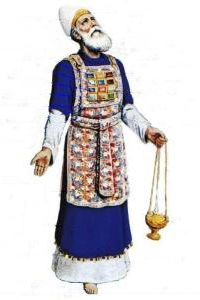
\includegraphics[width=50mm,scale=1.5]{Extras/Melchisedec.jpg}
\vspace{0.4in}  % Create a title for the document and write it in bold font
\LARGE{\textbf{\date}} % Again, do a line break
\linebreak 
% Create a subtitle \large{with Outlines, Statistics, Cross References, and Notes}
\vspace{0.5in}
\begin{flushleft}
\LARGE{Day \#99: Saturday, 9 April 2022 LITE  \\}\vspace{0.25in}
\LARGE{2 Samuel 19-21 Psalm 99 Proverb 9}
\end{flushleft}
\vspace{0.6in}
\bigskip

\normalsize{Xenia, Oh.\\}
\normalsize{created: \today}
\vspace{1.3in}

\end{flushright}
\end{titlepage}

\newpage 
\tableofcontents\hypertarget{TOC}{}
\listoffigures
\listoftables

\hyphenation{A-bim-e-lech bre-thren E-phra-im  Gib-e-o-nites Jer-u-sa-lem through-out Phil-i-stines The-o-phil-us Am-a-le-kites ven-geance Mesh-el-e-mi-ah onan-ism Phar-a-oh thoughts grev-ous-ness Hach-a-liah adul-ter-er Shad-rach}

%%%%%%%%%%%%%%%%% EXTRA COLORS
%%%%%%%%%%%%%%%%% EXTRA COLORS
%%%%%%%%%%%%%%%%% EXTRA COLORS
\definecolor{champagne}{rgb}{0.97,0.91,0.81}
\definecolor{bone}{rgb}{0.89,0.85,0.79}

\definecolor{ForestGreen}{rgb}{0.00,0.29,0.098}
\definecolor{GIVING}{cmyk}{1,0.0,0.72,.1}

\definecolor{MLPE}{cmyk}{1,1,0,.45}
\definecolor{SOCCER}{cmyk}{.77, 0, .42, .49}
\definecolor{PAYBILL}{cmyk}{0,0.83,0.76,0.07}
\definecolor{SERMON}{cmyk}{.14,.9,0,.30} % aka seance \href{http://www.flatuicolorpicker.com/purple-cmyk-color-model/}{seance}
\definecolor{BIBLE}{cmyk}{0,.17,.74,.17}
\definecolor{WORKBLUE}{cmyk}{1, .5, 0, .6}
\definecolor{myOrange}{cmyk}{0, .4, .98, .03}
\definecolor{myTan}{cmyk}{0.0,.07,.17,.10}
\definecolor{myRed}{cmyk}{0,1,1,0}
\definecolor{myWhite}{cmyk}{0,0,0,0}
\definecolor{BLUESoD}{cmyk}{.97,.84,0,.04}
\definecolor{WHITE}{cmyk}{0,0,0,0}
\definecolor{OLDGOLD}{cmyk}{0.05,0.3,1.00,0}
\definecolor{CASTLETON}{cmyk}{1,0,0.31,0.66}
\definecolor{cadmiumgreen}{rgb}{0.0, 0.42, 0.24}
\definecolor{jungle}{rgb}{0.203,0.4882,0.1718}
\definecolor{MYGOLD}{rgb}{1,.84,0}

\definecolor{MYLIGHTGRAY}{rgb}{.85,.85,.85}

\definecolor{codegreen}{rgb}{0,0.6,0}
\definecolor{codegray}{rgb}{0.5,0.5,0.5}
\definecolor{codepurple}{rgb}{0.58,0,0.82}
\definecolor{backcolour}{rgb}{0.95,0.95,0.92}


\mdfdefinestyle{MyFrame}{%
    linecolor=blue,
    outerlinewidth=2pt,
    roundcorner=5pt,
    innertopmargin=\baselineskip,
    innerbottommargin=\baselineskip,
    innerrightmargin=10pt,
    innerleftmargin=10pt,
    backgroundcolor=gray!25!white}


\mdfdefinestyle{MyFrame2}{%
    linecolor=black,
    outerlinewidth=2pt,
    roundcorner=5pt,
    innertopmargin=\baselineskip,
    innerbottommargin=\baselineskip,
    innerrightmargin=10pt,
    innerleftmargin=10pt,
    backgroundcolor=yellow!25!white}


%%%%%
%% for PFTTIS list
%%%%%

%%% And Joseph said unto
\index[PFTTIS]{And Joseph said unto!Genesis!Gen 40:008}
\index[PFTTIS]{And Joseph said unto!Genesis!Gen 40:012}
\index[PFTTIS]{And Joseph said unto!Genesis!Gen 41:025}
\index[PFTTIS]{And Joseph said unto!Genesis!Gen 42:014}
\index[PFTTIS]{And Joseph said unto!Genesis!Gen 42:018}
\index[PFTTIS]{And Joseph said unto!Genesis!Gen 44:015}
\index[PFTTIS]{And Joseph said unto!Genesis!Gen 45:003}
\index[PFTTIS]{And Joseph said unto!Genesis!Gen 45:004}
\index[PFTTIS]{And Joseph said unto!Genesis!Gen 46:031}
\index[PFTTIS]{And Joseph said unto!Genesis!Gen 48:009}
\index[PFTTIS]{And Joseph said unto!Genesis!Gen 48:018}
\index[PFTTIS]{And Joseph said unto!Genesis!Gen 50:019}
\index[PFTTIS]{And Joseph said unto!Genesis!Gen 50:024}


%%% a shadow
\index[PFTTIS]{a shadow!1Chronicles!1Chr 029:15}
\index[PFTTIS]{a shadow!Job!Job 008:09}
\index[PFTTIS]{a shadow!Job!Job 014:02}
\index[PFTTIS]{a shadow!Job!Job 017:07}
\index[PFTTIS]{a shadow!Psalm!Psa 102:011}
\index[PFTTIS]{a shadow!Psalm!Psa 144:004}
\index[PFTTIS]{a shadow!Ecclesiastes!Eccl 006:012}
\index[PFTTIS]{a shadow!Ecclesiastes!Eccl 008:013}
\index[PFTTIS]{a shadow!Isaiah!Isa 04:006}
\index[PFTTIS]{a shadow!Isaiah!Isa 25:004}
\index[PFTTIS]{a shadow!Jonah!Jnh 04:06}
\index[PFTTIS]{a shadow!Colossians!Col 02:017}
\index[PFTTIS]{a shadow!Hebews!Heb 10:001}

%%% blessed is the man
\index[PFTTIS]{blessed is the man!Psalm!Psa 001:001}
\index[PFTTIS]{blessed is the man!Psalm!Psa 032:002}
\index[PFTTIS]{blessed is the man!Psalm!Psa 034:008}
\index[PFTTIS]{blessed is the man!Psalm!Psa 065:004}
\index[PFTTIS]{blessed is the man!Psalm!Psa 084:005}
\index[PFTTIS]{blessed is the man!Psalm!Psa 084:012}
\index[PFTTIS]{blessed is the man!Psalm!Psa 094:012}
\index[PFTTIS]{blessed is the man!Psalm!Psa 112:001}
\index[PFTTIS]{blessed is the man!Proverbs!Pro 008:034}
\index[PFTTIS]{blessed is the man!Isaiah!Isa 056:002}
\index[PFTTIS]{blessed is the man!Jeremiah!Jer 017:007}
\index[PFTTIS]{blessed is the man!Romans!Rom 004:008}
\index[PFTTIS]{blessed is the man!James!Jam 001:012}


%%% carry them
\index[PFTTIS]{carry them!Leviticus!Lev 14:045}
\index[PFTTIS]{carry them!Numbers!Num 11:012}
\index[PFTTIS]{carry them!Joshua!Jsh 04:003}
\index[PFTTIS]{carry them!1Samuel!1Sam 20:040}
\index[PFTTIS]{carry them!1Kings!1Kng 08:046}
\index[PFTTIS]{carry them!2Chronicles!2Chr 06:036}
\index[PFTTIS]{carry them!Ezra!Ezra 05:015}
\index[PFTTIS]{carry them!Isaiah!Isa 40:011}
\index[PFTTIS]{carry them!Isaiah!Isa 41:016}
\index[PFTTIS]{carry them!Isaiah!Isa 57:013}
\index[PFTTIS]{carry them!Jeremiah!Jer 20:004}
\index[PFTTIS]{carry them!Jeremiah!Jer 20:005}
\index[PFTTIS]{carry them!Jeremiah!Jer 43:012}


\index[PFTTIS]{good tidings!2Samuel!2Sam 18:027}
\index[PFTTIS]{good tidings!1Kings!1Ki 01:042}
\index[PFTTIS]{good tidings!2Kings!2Ki 07:009 (2x)}
\index[PFTTIS]{good tidings!Isaiah!Isa 40:009 (2x)}
\index[PFTTIS]{good tidings!Isaiah!Isa 41:007}
\index[PFTTIS]{good tidings!Isaiah!Isa 52:007}
\index[PFTTIS]{good tidings!Isaiah!Isa 61:001}
\index[PFTTIS]{good tidings!Nahum!Nah 01:005}
\index[PFTTIS]{good tidings!Luke!Lk 02:010}
\index[PFTTIS]{good tidings!1Thessalonians!1Thess 03:006}


%%% dead body
\index[PFTTIS]{dead body!Leviticus!Lev 21:011}
\index[PFTTIS]{dead body!Numbers!Num 06:006}
\index[PFTTIS]{dead body!Numbers!Num 09:006}
\index[PFTTIS]{dead body!Numbers!Num 09:007}
\index[PFTTIS]{dead body!Numbers!Num 09:010}
\index[PFTTIS]{dead body!Numbers!Num 09:011}
\index[PFTTIS]{dead body!Numbers!Num 09:013}
\index[PFTTIS]{dead body!Numbers!Num 09:016}
\index[PFTTIS]{dead body!2Kings!2Ki 08:005}
\index[PFTTIS]{dead body!Isaiah!Isa 26:019}
\index[PFTTIS]{dead body!Jeremiah!Jer 26:023}
\index[PFTTIS]{dead body!Jeremiah!Jer 36:030}
\index[PFTTIS]{dead body!Haggai!Hag 02:013}

%%% great sea
\index[PFTTIS]{great sea!Numbers!Num 34:006}
\index[PFTTIS]{great sea!Numbers!Num 34:007}
\index[PFTTIS]{great sea!Joshua!Jos 01:004}
\index[PFTTIS]{great sea!Joshua!Jos 09:001}
\index[PFTTIS]{great sea!Joshua!Jos 15:012}
\index[PFTTIS]{great sea!Joshua!Jos 15:047}
\index[PFTTIS]{great sea!Joshua!Jos 23:004}
\index[PFTTIS]{great sea!Ezekiel!Eze 47:010}
\index[PFTTIS]{great sea!Ezekiel!Eze 47:015}
\index[PFTTIS]{great sea!Ezekiel!Eze 47:019}
\index[PFTTIS]{great sea!Ezekiel!Eze 47:020}
\index[PFTTIS]{great sea!Ezekiel!Eze 48:028}
\index[PFTTIS]{great sea!Daniel!Dan 07:002}


%%% have forsaken me
\index[PFTTIS]{have forsaken me!Judges!Jdg 10:013}
\index[PFTTIS]{have forsaken me!1Samuel!1Sam 08:008}
\index[PFTTIS]{have forsaken me!1Kings!1Ki 11:033}
\index[PFTTIS]{have forsaken me!2Kings!2Ki 22:017}
\index[PFTTIS]{have forsaken me!2Chronicles!2Chr 12:005}
\index[PFTTIS]{have forsaken me!2Chronicles!2Chr 34:025}
\index[PFTTIS]{have forsaken me!Jeremiah!Jer 01:016}
\index[PFTTIS]{have forsaken me!Jeremiah!Jer 02:013}
\index[PFTTIS]{have forsaken me!Jeremiah!Jer 05:007}
\index[PFTTIS]{have forsaken me!Jeremiah!Jer 05:019}
\index[PFTTIS]{have forsaken me!Jeremiah!Jer 16:011 (2x)}
\index[PFTTIS]{have forsaken me!Jeremiah!Jer 19:004}

%%% no king
\index[PFTTIS]{no king!Judges!Jdg 17:06}
\index[PFTTIS]{no king!Judges!Jdg 18:01}
\index[PFTTIS]{no king!Judges!Jdg 19:01}
\index[PFTTIS]{no king!Judges!Jdg 21:25}
\index[PFTTIS]{no king!1Kings!1Ki 22:47}
\index[PFTTIS]{no king!2Kings!2Ki 23:25}
\index[PFTTIS]{no king!Nehemiah!Neh 13:26}
\index[PFTTIS]{no king!Psalms!Psa 033:016}
\index[PFTTIS]{no king!Proverbs!Pro 30:27}
\index[PFTTIS]{no king!Daniel!Dan 02:10}
\index[PFTTIS]{no king!Hosea!Hos 10:03}
\index[PFTTIS]{no king!Micah!Mic 04:09}
\index[PFTTIS]{no king!John!Jhn 19:15}


%%% rebellious house
\index[PFTTIS]{rebellious house!Exodus!Exo 02:005}
\index[PFTTIS]{rebellious house!Exodus!Exo 02:006}
\index[PFTTIS]{rebellious house!Exodus!Exo 02:008}
\index[PFTTIS]{rebellious house!Exodus!Exo 03:009}
\index[PFTTIS]{rebellious house!Exodus!Exo 03:026}
\index[PFTTIS]{rebellious house!Exodus!Exo 03:027}
\index[PFTTIS]{rebellious house!Exodus!Exo 12:002 (2x)}
\index[PFTTIS]{rebellious house!Exodus!Exo 12:003}
\index[PFTTIS]{rebellious house!Exodus!Exo 12:009}
\index[PFTTIS]{rebellious house!Exodus!Exo 12:025}
\index[PFTTIS]{rebellious house!Exodus!Exo 17:012}
\index[PFTTIS]{rebellious house!Exodus!Exo 24:003}

%%% seek him
\index[PFTTIS]{seek him!Deuteronomy!Deu 04:029}\index[PFTTIS]{seek him!1Samuel!1Sam 23:025}
\index[PFTTIS]{seek him!1Chronicles!1Chr 28:009}
\index[PFTTIS]{seek him!2Chronicles!1Chr 15:002}
\index[PFTTIS]{seek him!Ezra!Ezr 08:022}
\index[PFTTIS]{seek him!Psalms!Psa 022:026}
\index[PFTTIS]{seek him!Psalms!Psa 024:006}
\index[PFTTIS]{seek him!Psalms!Psa 119:002}
\index[PFTTIS]{seek him!SoS!SoS 03:002}
\index[PFTTIS]{seek him!SoS!SoS 06:001}
\index[PFTTIS]{seek him!Hosea!Hos 07:010}
\index[PFTTIS]{seek him!Amos!Amo 05:008}
\index[PFTTIS]{seek him!Hebrews!Heb 11:0063}


%%% seek ye
\index[PFTTIS]{seek ye!Isaiah!Isa 34:016}
\index[PFTTIS]{seek ye!Isaiah!Isa 45:019}
\index[PFTTIS]{seek ye!Isaiah!Isa 55:006}
\index[PFTTIS]{seek ye!Amos!Amos 5:004}
\index[PFTTIS]{seek ye!John!John 1:38}
\index[PFTTIS]{seek ye!John!John 18:4}
\index[PFTTIS]{seek ye!John!John 18:7}
\index[PFTTIS]{seek ye!Matthew!Matt 6:33}
\index[PFTTIS]{seek ye!Numbers!Num 16:10}
\index[PFTTIS]{seek ye!Luke!Luke 12:31}
\index[PFTTIS]{seek ye!Luke!Luke 24:5}
\index[PFTTIS]{seek ye!Psalm!Psa 27:8}
\index[PFTTIS]{seek ye!Zephaniah!Zeph 2:3}

%%% the uncircumcised
\index[PFTTIS]{the uncircumcised!Genesis!Gen 17:014}
\index[PFTTIS]{the uncircumcised!Judges!Jdg 14:003}
\index[PFTTIS]{the uncircumcised!Judges!Jdg 15:018}
\index[PFTTIS]{the uncircumcised!2Samuel!2Sam 01:020}
\index[PFTTIS]{the uncircumcised!Isaiah!Isa 02:001}
\index[PFTTIS]{the uncircumcised!Jeremiah!Jer 09:025}
\index[PFTTIS]{the uncircumcised!Ezekiel!Eze 28:010}
\index[PFTTIS]{the uncircumcised!Ezekiel!Eze 31:018}
\index[PFTTIS]{the uncircumcised!Ezekiel!Eze 32:019}
\index[PFTTIS]{the uncircumcised!Ezekiel!Eze 32:027}
\index[PFTTIS]{the uncircumcised!Ezekiel!Eze 32:028}
\index[PFTTIS]{the uncircumcised!Ezekiel!Eze 32:029}
\index[PFTTIS]{the uncircumcised!Ezekiel!Eze 32:032}

%%% worship him
\index[PFTTIS]{worship him!Psalms!Psa 97:007}
\index[PFTTIS]{worship him!Zephaniah!Zeph 02:011}
\index[PFTTIS]{worship him!Matthew!Matt 02:002}
\index[PFTTIS]{worship him!Matthew!Matt 02:008}
\index[PFTTIS]{worship him!John!John 04:023}
\index[PFTTIS]{worship him!John!John 04:024 (2x)} 
\index[PFTTIS]{worship him!Acts!Acts 17:023}
\index[PFTTIS]{worship him!Hebrews!Heb 01:006}
\index[PFTTIS]{worship him!Revelation!Rev 04:010}
\index[PFTTIS]{worship him!Revelation!Rev 13:008}
\index[PFTTIS]{worship him!Revelation!Rev 14:007}
\index[PFTTIS]{worship him!Revelation!Rev 19:010}


%%%%%
%% for PFTTIS list
%%%%%

%%% afflictions
\index[WFTTIS]{afflictions!Psalms!Psa 34:019}
\index[WFTTIS]{afflictions!Psalms!Psa 132:001}
\index[WFTTIS]{afflictions!Acts!Acts 07:010}
\index[WFTTIS]{afflictions!Acts!Acts 20:023}
\index[WFTTIS]{afflictions!2Corinthians!2Cor 06:004}
\index[WFTTIS]{afflictions!Colossians!Col 01:024}
\index[WFTTIS]{afflictions!1Thessalonians!1Thess 03:003}
\index[WFTTIS]{afflictions!2Timothy!2Tim 01:008}
\index[WFTTIS]{afflictions!2Timothy!2Tim 03:011}
\index[WFTTIS]{afflictions!2Timothy!2Tim 04:005}
\index[WFTTIS]{afflictions!Hebrews!Heb 10:032}
\index[WFTTIS]{afflictions!Hebrews!Heb 10:033}
\index[WFTTIS]{afflictions!1Peter!1Pet 05:009}

%%% acsend
\index[WFTTIS]{acsend!Joshua!Jos 06:05}
\index[WFTTIS]{acsend!Psalm!Psa 024:003}
\index[WFTTIS]{acsend!Psalm!Psa 135:007}
\index[WFTTIS]{acsend!Psalm!Psa 139:008}
\index[WFTTIS]{acsend!Isaiah!Isa 14:013}
\index[WFTTIS]{acsend!Isaiah!Isa 14:014}
\index[WFTTIS]{acsend!Jeremiah!Jer 10:013}
\index[WFTTIS]{acsend!Jeremiah!Jer 51:016}
\index[WFTTIS]{acsend!Ezekiel!Eze 38:009}
\index[WFTTIS]{acsend!John!John 06:062}
\index[WFTTIS]{acsend!John!John 20:017}
\index[WFTTIS]{acsend!Romans!Rom 10:006}
\index[WFTTIS]{acsend!Revelation!Rev 17:008}

%%% Assyrian
\index[WFTTIS]{Assyrian!Isaiah!Isa 10:005}
\index[WFTTIS]{Assyrian!Isaiah!Isa 10:024}
\index[WFTTIS]{Assyrian!Isaiah!Isa 14:025}
\index[WFTTIS]{Assyrian!Isaiah!Isa 19:023}
\index[WFTTIS]{Assyrian!Isaiah!Isa 23:013}
\index[WFTTIS]{Assyrian!Isaiah!Isa 30:031}
\index[WFTTIS]{Assyrian!Isaiah!Isa 31:008}
\index[WFTTIS]{Assyrian!Isaiah!Isa 52:004}
\index[WFTTIS]{Assyrian!Ezekiel!Eze 31:003}
\index[WFTTIS]{Assyrian!Hosea!Hos 05:013}
\index[WFTTIS]{Assyrian!Hosea!Hos 11:005}
\index[WFTTIS]{Assyrian!Micah!Hos 05:005}
\index[WFTTIS]{Assyrian!Micah!Hos 05:006}

%%% blot
\index[WFTTIS]{blot!Exodus!Exo 32:032}
\index[WFTTIS]{blot!Exodus!Exo 32:033}
\index[WFTTIS]{blot!Numbers!Num 05:026}
\index[WFTTIS]{blot!Deuteronomy!Deut 09:014}
\index[WFTTIS]{blot!Deuteronomy!Deut 25:019}
\index[WFTTIS]{blot!Deuteronomy!Deut 29:020}
\index[WFTTIS]{blot!2Kings!2Ki 14:027}
\index[WFTTIS]{blot!Job!Job 31:007}
\index[WFTTIS]{blot!Psalms!Psa 51:001}
\index[WFTTIS]{blot!Psalms!Psa 51:009}
\index[WFTTIS]{blot!Proverbs!Pro 09:007}
\index[WFTTIS]{blot!Jeremiah!Jer 18:023}
\index[WFTTIS]{blot!Revelation!Rev 03:005}


%%% chain
\index[WFTTIS]{chain!Genesis!Gen 41:042}
\index[WFTTIS]{chain!1Kings!1Ki 07:017}
\index[WFTTIS]{chain!Psalms!Psa 73:006}
\index[WFTTIS]{chain!SoS!Sos 04:009}
\index[WFTTIS]{chain!Lamentations!Lam 03:007}
\index[WFTTIS]{chain!Ezekiel!Eze 07:023}
\index[WFTTIS]{chain!Ezekiel!Eze 16:011}
\index[WFTTIS]{chain!Daniel!Dan 05:007}
\index[WFTTIS]{chain!Daniel!Dan 05:016}
\index[WFTTIS]{chain!Daniel!Dan 05:029}
\index[WFTTIS]{chain!Acts!Acts 28:020}
\index[WFTTIS]{chain!2Timothy!2Tim 01:016}
\index[WFTTIS]{chain!Revelation!Rev 20:001}


%%% controversy
\index[WFTTIS]{controversy!Deuteronomy!Deu 17:008}
\index[WFTTIS]{controversy!Deuteronomy!Deu 19:017}
\index[WFTTIS]{controversy!Deuteronomy!Deu 21:005}
\index[WFTTIS]{controversy!Deuteronomy!Deu 25:001}
\index[WFTTIS]{controversy!2Samuel!2Sam 15:002}
\index[WFTTIS]{controversy!Isaiah!Isa 34:008}
\index[WFTTIS]{controversy!Jeremiah!Jer 25:031}
\index[WFTTIS]{controversy!Ezekiel!Eze 44:024}
\index[WFTTIS]{controversy!Hosea!Hos 04:001}
\index[WFTTIS]{controversy!Hosea!Hos 12:002}
\index[WFTTIS]{controversy!Micah!Mic 06:002 (2x)}
\index[WFTTIS]{controversy!1Timothy!1Tim 03:016}


%%% Dagon/Dagon's
\index[WFTTIS]{Dagon!Judges!Jdg 16:023}
\index[WFTTIS]{Dagon!1Samuel!1Sam 05:002 (2x)}
\index[WFTTIS]{Dagon!1Samuel!1Sam 05:003 (2x)}
\index[WFTTIS]{Dagon!1Samuel!1Sam 05:004 (3x)}
\index[WFTTIS]{Dagon!1Samuel!1Sam 05:005 (3x)}
\index[WFTTIS]{Dagon!1Samuel!1Sam 05:007}
\index[WFTTIS]{Dagon!1Chronicles!1Chr 10:010}

%%% disobedient
\index[WFTTIS]{disobedient!1Kings!1Ki 13:026}
\index[WFTTIS]{disobedient!Nehemiah!Neh 09:026}
\index[WFTTIS]{disobedient!Luke!Luke 01:017}
\index[WFTTIS]{disobedient!Acts!Acts 26:019}
\index[WFTTIS]{disobedient!Romans!Rom 01:030}
\index[WFTTIS]{disobedient!Romans!Rom 10:021}
\index[WFTTIS]{disobedient!1Timothy!1Tim 01:009}
\index[WFTTIS]{disobedient!2Timothy!2Tim 03:002}
\index[WFTTIS]{disobedient!Titus!Titus 01:016}
\index[WFTTIS]{disobedient!Titus!Titus 03:003}
\index[WFTTIS]{disobedient!1Peter!1Pet 02:007}
\index[WFTTIS]{disobedient!1Peter!1Pet 02:008}
\index[WFTTIS]{disobedient!1Peter!1Pet 03:020}


%%% doubt
\index[WFTTIS]{doubt!Genesis!Gen 37:033}
\index[WFTTIS]{doubt!Deuteronomy!Deu 28:066}
\index[WFTTIS]{doubt!Job!Job 12:002}
\index[WFTTIS]{doubt!Matthew!Matt 14:031}
\index[WFTTIS]{doubt!Matthew!Matt 21:021}
\index[WFTTIS]{doubt!Mark!Mk 11:023}
\index[WFTTIS]{doubt!Luke!Lk 11:020}
\index[WFTTIS]{doubt!John!Jhn 10:024}
\index[WFTTIS]{doubt!Acts!Acts 02:012}
\index[WFTTIS]{doubt!Acts!Acts 28:004}
\index[WFTTIS]{doubt!1Corinthians!1Cor 09:010}
\index[WFTTIS]{doubt!Galatians!Gal 04:020}
\index[WFTTIS]{doubt!1John!1Jhn 02:019}


%%% dungeon
\index[WFTTIS]{dungeon!Genesis!Gen 40:015}
\index[WFTTIS]{dungeon!Genesis!Gen 41:014}
\index[WFTTIS]{dungeon!Exodus!Exo 12:029}
\index[WFTTIS]{dungeon!Jeremiah!Jer 37:016}
\index[WFTTIS]{dungeon!Jeremiah!Jer 38:006 (2x)}
\index[WFTTIS]{dungeon!Jeremiah!Jer 38:007}
\index[WFTTIS]{dungeon!Jeremiah!Jer 38:009}
\index[WFTTIS]{dungeon!Jeremiah!Jer 38:010}
\index[WFTTIS]{dungeon!Jeremiah!Jer 38:011}
\index[WFTTIS]{dungeon!Jeremiah!Jer 38:013}
\index[WFTTIS]{dungeon!Lamentations!Lam 03:053}
\index[WFTTIS]{dungeon!Lamentations!Lam 03:055}


%%% error
\index[WFTTIS]{error!2Samuel!2Sam 06:007}
\index[WFTTIS]{error!Job!Job 19:004}
\index[WFTTIS]{error!Ecclesiastes!Ecc 05:006}
\index[WFTTIS]{error!Ecclesiastes!Ecc 10:005}
\index[WFTTIS]{error!Isaiah!Isa 32:006}
\index[WFTTIS]{error!Daniel!Dan 06:004}
\index[WFTTIS]{error!Matthew!Matt 27:064}
\index[WFTTIS]{error!Romans!Rom 01:027}
\index[WFTTIS]{error!James!Jam 05:020}
\index[WFTTIS]{error!2Peter!2Pet 02:018}
\index[WFTTIS]{error!2Peter!2Pet 03:017}
\index[WFTTIS]{error!1John!1Jn 04:006}
\index[WFTTIS]{error!Jude!Jude 01:011}

%%% fourish
\index[WFTTIS]{fourish!Psalms!Psa 072:007}
\index[WFTTIS]{fourish!Psalms!Psa 072:016}
\index[WFTTIS]{fourish!Psalms!Psa 092:007}
\index[WFTTIS]{fourish!Psalms!Psa 092:012}
\index[WFTTIS]{fourish!Psalms!Psa 092:013}
\index[WFTTIS]{fourish!Psalms!Psa 132:018}
\index[WFTTIS]{fourish!Proverbs!Pro 11:28}
\index[WFTTIS]{fourish!Proverbs!Pro 14:11}
\index[WFTTIS]{fourish!Ecclesiastes!Ecc 12:05}
\index[WFTTIS]{fourish!SongOfSolomon!SOS 07:12}
\index[WFTTIS]{fourish!Isaiah!Isa 17:11}
\index[WFTTIS]{fourish!Isaiah!Isa 66:14}
\index[WFTTIS]{fourish!Ezekiel!Eze 17:24}




%%% giants
\index[WFTTIS]{giants!Genesis!Gen 06:004}
\index[WFTTIS]{giants!Numbers!Num 13:033}
\index[WFTTIS]{giants!Deuteronomy!Deut 02:011}
\index[WFTTIS]{giants!Deuteronomy!Deut 02:021}
\index[WFTTIS]{giants!Deuteronomy!Deut 03:011}
\index[WFTTIS]{giants!Deuteronomy!Deut 03:013}
\index[WFTTIS]{giants!Joshua!Josh 12:004}
\index[WFTTIS]{giants!Joshua!Josh 13:012}
\index[WFTTIS]{giants!Joshua!Josh 15:008}
\index[WFTTIS]{giants!Joshua!Josh 17:015}
\index[WFTTIS]{giants!Joshua!Josh 16:016}

%%% good man
\index[WFTTIS]{good man!2 Samuel!2Sa 18:27}
%(1) Psalms 37:23 [5]
%(1) Psalms 112:5 [2]
%(1) Proverbs 12:2 [2]
%(1) Proverbs 13:22 [2]
%(1) Proverbs 14:14 [14]
%(1) Micah 7:2 [2]
%(1) Matthew 12:35 [2]
%(1) Luke 6:45 [2]
%(1) Luke 23:50 [15]
%(1) John 7:12 [17]
%(1) Acts 11:24 [5]
%(1) Romans 5:7 [14]

%%% Hinnom
\index[WFTTIS]{Hinnom!Joshua!Jsh 15:008}
\index[WFTTIS]{Hinnom!Joshua!Jsh 18:016}
\index[WFTTIS]{Hinnom!2Kings!2Ki 23:010}
\index[WFTTIS]{Hinnom!2Chronicles!2Chr 28:003}
\index[WFTTIS]{Hinnom!2Chronicles!2Chr 33:006}
\index[WFTTIS]{Hinnom!Nehemiah!Neh 11:030}
\index[WFTTIS]{Hinnom!Jeremiah!Jer 07:031}
\index[WFTTIS]{Hinnom!Jeremiah!Jer 07:032}
\index[WFTTIS]{Hinnom!Jeremiah!Jer 19:002}
\index[WFTTIS]{Hinnom!Jeremiah!Jer 19:006}
\index[WFTTIS]{Hinnom!Jeremiah!Jer 32:035}

%%% inclined
\index[WFTTIS]{inclined!Judges!Jdg 09:003}
\index[WFTTIS]{inclined!Psalms!Psa 040:001}
\index[WFTTIS]{inclined!Psalms!Psa 116:002}
\index[WFTTIS]{inclined!Psalms!Psa 119:112}
\index[WFTTIS]{inclined!Proverbs!Pro 05:13}
\index[WFTTIS]{inclined!Jeremiah!Jer 07:24}
\index[WFTTIS]{inclined!Jeremiah!Jer 07:26}
\index[WFTTIS]{inclined!Jeremiah!Jer 11:08}
\index[WFTTIS]{inclined!Jeremiah!Jer 17:23}
\index[WFTTIS]{inclined!Jeremiah!Jer 25:04}
\index[WFTTIS]{inclined!Jeremiah!Jer 34:14}
\index[WFTTIS]{inclined!Jeremiah!Jer 35:15}
\index[WFTTIS]{inclined!Jeremiah!Jer 44:05}


%%% laughed
\index[WFTTIS]{laughed!Genesis!Gen 17:017}
\index[WFTTIS]{laughed!Genesis!Gen 18:012}
\index[WFTTIS]{laughed!Genesis!Gen 18:015}
\index[WFTTIS]{laughed!2Kings!2Ki 19:021}
\index[WFTTIS]{laughed!2Chronicles!2Chr 30:010}
\index[WFTTIS]{laughed!Nehemiah!Neh 02:019}
\index[WFTTIS]{laughed!Job!Job 12:004}
\index[WFTTIS]{laughed!Job!Job 29:024}
\index[WFTTIS]{laughed!Isaiah!Isa 37:022}
\index[WFTTIS]{laughed!Ezekiel!Ezek 23:032}
\index[WFTTIS]{laughed!Matthew!Matt 09:024}
\index[WFTTIS]{laughed!Mark!Mk 05:040}
\index[WFTTIS]{laughed!Luke!Lk 08:053}

%%% liar
\index[WFTTIS]{liar!Job!Job 24:025}
\index[WFTTIS]{liar!Proverbs!Pro 17:004}
\index[WFTTIS]{liar!Proverbs!Pro 19:022}
\index[WFTTIS]{liar!Proverbs!Pro 30:006}
\index[WFTTIS]{liar!Jeremiah!Jer 15:018}
\index[WFTTIS]{liar!John!Jhn 08:044}
\index[WFTTIS]{liar!John!Jhn 08:055}
\index[WFTTIS]{liar!Romans!Rom 03:004}
\index[WFTTIS]{liar!1John!1Jhn 01:010}
\index[WFTTIS]{liar!1John!1Jhn 02:004}
\index[WFTTIS]{liar!1John!1Jhn 02:022}
\index[WFTTIS]{liar!1John!1Jhn 04:020}
\index[WFTTIS]{liar!1John!1Jhn 05:010}

%%% palsy
\index[WFTTIS]{palsy!Matthew!Matt 04:024}
\index[WFTTIS]{palsy!Matthew!Matt 08:006}
\index[WFTTIS]{palsy!Matthew!Matt 09:002}
\index[WFTTIS]{palsy!Matthew!Matt 09:006}
\index[WFTTIS]{palsy!Mark!Mk 02:003}
\index[WFTTIS]{palsy!Mark!Mk 02:004}
\index[WFTTIS]{palsy!Mark!Mk 02:005}
\index[WFTTIS]{palsy!Mark!Mk 02:009}
\index[WFTTIS]{palsy!Mark!Mk 02:010}
\index[WFTTIS]{palsy!Luke!Lk 05:018}
\index[WFTTIS]{palsy!Luke!Lk 05:024}
\index[WFTTIS]{palsy!Acts!Acts 09:033}

%%% Profitable
\index[WFTTIS]{profitable!Job!Job 22:002 (2x)}
\index[WFTTIS]{profitable!Ecclesiastes!Ecc 10:010}
\index[WFTTIS]{profitable!Isaiah!Isa 44:010}
\index[WFTTIS]{profitable!Jeremiah!Jer 13:007}
\index[WFTTIS]{profitable!Matthew!Matt 05:029}
\index[WFTTIS]{profitable!Matthew!Matt 05:030}
\index[WFTTIS]{profitable!Acts!Acts 20:020}
\index[WFTTIS]{profitable!1Timothy!1Tim 04:008}
\index[WFTTIS]{profitable!2Timothy!2Tim 03:016}
\index[WFTTIS]{profitable!2Timothy!2Tim 04:011}
\index[WFTTIS]{profitable!Titus!Titus 03:008}
\index[WFTTIS]{profitable!Philemon!Phlm 01:011}

%%% Rechab
\index[WFTTIS]{Rechab!2Samuel!2Sam 04:002}
\index[WFTTIS]{Rechab!2Samuel!2Sam 04:005}
\index[WFTTIS]{Rechab!2Samuel!2Sam 04:006}
\index[WFTTIS]{Rechab!2Samuel!2Sam 04:009}
\index[WFTTIS]{Rechab!2KIngs!2Ki 10:015}
\index[WFTTIS]{Rechab!2KIngs!2Ki 10:023}
\index[WFTTIS]{Rechab!1Chronicles!1Chr 02:055}
\index[WFTTIS]{Rechab!Nehemiah!Neh 03:014}
\index[WFTTIS]{Rechab!Jeremiah!Jer 35:006}
\index[WFTTIS]{Rechab!Jeremiah!Jer 35:008}
\index[WFTTIS]{Rechab!Jeremiah!Jer 35:014}
\index[WFTTIS]{Rechab!Jeremiah!Jer 35:016}
\index[WFTTIS]{Rechab!Jeremiah!Jer 35:019}

%%% serpents
\index[WFTTIS]{serpents!Exodus!Exo 07:012}
\index[WFTTIS]{serpents!Numbers!Num 21:006}
\index[WFTTIS]{serpents!Numbers!Num 21:007}
\index[WFTTIS]{serpents!Deuteronomy!Deu 08:015}
\index[WFTTIS]{serpents!Deuteronomy!Deu 32:024}
\index[WFTTIS]{serpents!Jeremiah!Jer 08:017}
\index[WFTTIS]{serpents!Matthew!Matt 10:016}
\index[WFTTIS]{serpents!Matthew!Matt 23:033}
\index[WFTTIS]{serpents!Mark!Mk 16:018}
\index[WFTTIS]{serpents!Luke!Lk 10:019}
\index[WFTTIS]{serpents!1Corinthians!1Cor 10:009}
\index[WFTTIS]{serpents!James!Jas 03:007}
\index[WFTTIS]{serpents!Revelation!Rev 09:019}

%%% short
\index[WFTTIS]{short!Numbers!Num 11:023}
\index[WFTTIS]{short!2Kings!2Ki 10:032}
\index[WFTTIS]{short!Job!Job 17:012}
\index[WFTTIS]{short!Job!Job 20:005}
\index[WFTTIS]{short!Psalms!Psa 89:047}
\index[WFTTIS]{short!Romans!Rom 03:023}
\index[WFTTIS]{short!Romans!Rom 09:028  (2x)}
\index[WFTTIS]{short!1Corinthians!1Cor 07:029}
\index[WFTTIS]{short!1Thessalonians!1Thess 02:017}
\index[WFTTIS]{short!Hebrews!Heb 04:001}
\index[WFTTIS]{short!Revelation!Rev 12:012}
\index[WFTTIS]{short!Revelation!Rev 17:010}

%%% smiteth
\index[WFTTIS]{smiteth!Exodus!Exo 21:012}
\index[WFTTIS]{smiteth!Exodus!Exo 21:15}
\index[WFTTIS]{smiteth!Deuteronomy!Dt 25:11}
\index[WFTTIS]{smiteth!Deuteronomy!Dt 27:24}
\index[WFTTIS]{smiteth!Joshua!Jsh 15:16}
\index[WFTTIS]{smiteth!Judges!Jdg 15:16}
\index[WFTTIS]{smiteth!2 Samuel!2Sa 05:08}
\index[WFTTIS]{smiteth!1Chronicles!1Chr 11:06}
\index[WFTTIS]{smiteth!Job!1Chr 26:12}
\index[WFTTIS]{smiteth!Isaiah!Isa 09:13}
\index[WFTTIS]{smiteth!Lamentations!Lam 03:30}
\index[WFTTIS]{smiteth!Ezekiel!Eze 07:09}
\index[WFTTIS]{smiteth!Luke!Lk 06:29}



%%% vanities
\index[WFTTIS]{vanities!Deuteronomy!Deut 21:021}
\index[WFTTIS]{vanities!1Kings!1Ki 16:013}
\index[WFTTIS]{vanities!1Kings!1Ki 16:026}
\index[WFTTIS]{vanities!Psalms!Psa 031:006}
\index[WFTTIS]{vanities!Ecclesiastes!Ecc 01:002 (2x)}
\index[WFTTIS]{vanities!Ecclesiastes!Ecc 05:007}
\index[WFTTIS]{vanities!Ecclesiastes!Ecc 12:008}
\index[WFTTIS]{vanities!Jeremiah!Jer 08:019}
\index[WFTTIS]{vanities!Jeremiah!Jer 10:008}
\index[WFTTIS]{vanities!Jeremiah!Jer 14:022}
\index[WFTTIS]{vanities!Jonah!Jnh 02:008}
\index[WFTTIS]{vanities!Acts!Acts 14:015}



%%%%%
%% for PFTTIS list
%%%%%

%%% worm
\index[WFITV]{worm!Exodus!Exo 16:024}
\index[WFITV]{worm!Job!Job 17:014}
\index[WFITV]{worm!Job!Job 24:029}
\index[WFITV]{worm!Job!Job 25:005 (2x)}
\index[WFITV]{worm!Psalms!Psa 022:006}
\index[WFITV]{worm!Isaiah!Isa 14:011}
\index[WFITV]{worm!Isaiah!Isa 41:014}
\index[WFITV]{worm!Isaiah!Isa 51:008}
\index[WFITV]{worm!Isaiah!Isa 66:024}
\index[WFITV]{worm!Jonah!Jnh 04:007}
\index[WFITV]{worm!Mark!Mk 09:044}
\index[WFITV]{worm!Mark!Mk 09:046}
\index[WFITV]{worm!Mark!Mk 09:048}


%\subsubsection{Title}
%\textbf{Introduction:} Isaiah 46 
%\index[speaker]{Speaker!Isaiah 49 (Title}
%\index[series]{Book (Speaker)!IPassage (Title)}
%\index[date]{2017/07/09!Isaiah 49 (Title)}
%\begin{compactenum}[I.]
%    \item  \textbf{Point} \index[scripture]{Isaiah!IPassage} (IPassage)
%\end{compactenum}




  

\chapter{2 Samuel 19}

\begin{figure}
  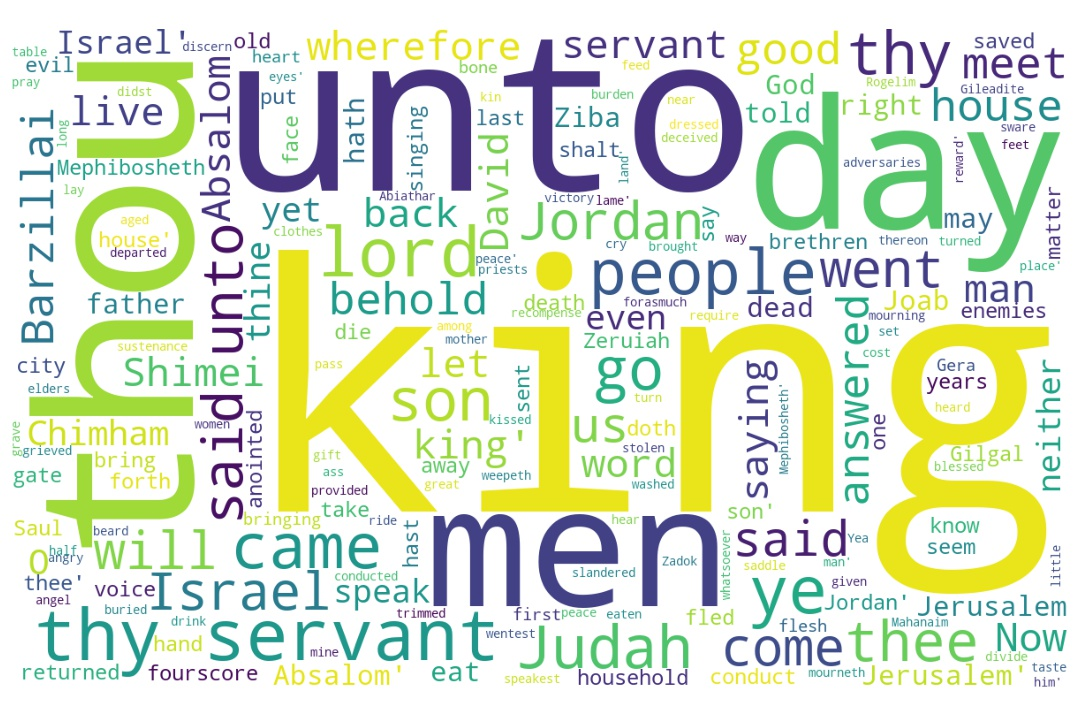
\includegraphics[width=\linewidth]{10OT-2Samuel/2Samuel19-WordCloud.jpg}
  \caption{1 Samuel 19 Word Cloud}
  \label{fig:1 Samuel 19 Word Cloud}
\end{figure}

%%%%%%%%%%%%%%%%%%%%%%%%%%%%%%%%%%%%%%%%%
%%%%%%%%%%%%%%%%%%%%%%%%%%%%%%%%%%%%%%%%%

\marginpar{\scriptsize \centering \fcolorbox{bone}{lime}{\textbf{NO TIME TO WEEP}}\\ (2 Samuel 19:1-43) \begin{compactenum}[I.][8]
   \item The  \textbf{Grief} \index[scripture]{2Samuel!2Sa 19:02} (2Sa 19:2) 
   \item The  \textbf{Gate} \index[scripture]{2Samuel!2Sa 19:08} (2Sa 19:8) 
   \item The  \textbf{Greeting} \index[scripture]{2Samuel!2Sa 19:15} (2Sa 19:15) 
   \item   \textbf{Guilt} Pardoned \index[scripture]{2Samuel!2Sa 19:23} (2Sa 19:23) 
   \item The  \textbf{Grave} \index[scripture]{2Samuel!2Sa 19:37} (2Sa 19:37) 
   \item Some  \textbf{Grace} \index[scripture]{2Samuel!2Sa 19:37} (2Sa 19:37) 
   \item A  \textbf{Gulf} Evident \index[scripture]{2Samuel!2Sa 19:41--43} (2Sa 19:41--43) 
\end{compactenum}}

\footnote{\textcolor[cmyk]{0.99998,1,0,0}{\hyperlink{TOC}{Return to end of Table of Contents.}}}\footnote{\href{https://audiobible.com/bible/2_samuel_19.html}{\textcolor[cmyk]{0.99998,1,0,0}{2 Samuel 19 Audio}}}\textcolor[cmyk]{0.99998,1,0,0}{And it was told Joab, Behold, the king weepeth and mourneth \fcolorbox{bone}{bone}{for} Absalom.}
[2] \textcolor[cmyk]{0.99998,1,0,0}{And the victory that day was \emph{turned} into mourning unto all the people: \fcolorbox{bone}{bone}{for} the people heard say that day how the king was \fcolorbox{bone}{lime}{grieved} \fcolorbox{bone}{bone}{for} his son.}
[3] \textcolor[cmyk]{0.99998,1,0,0}{And the people gat them by stealth that day into the city, as people being ashamed steal away when they flee in battle.}
[4] \textcolor[cmyk]{0.99998,1,0,0}{But the king covered his face, and the king cried with a loud voice, O my son Absalom, O Absalom, my son, my son!}
[5] \textcolor[cmyk]{0.99998,1,0,0}{And Joab came into the house to the king, and said, Thou hast shamed \fcolorbox{bone}{bone}{this} day the faces of all thy servants, which \fcolorbox{bone}{bone}{this} day have saved thy life, and the lives of thy sons and of thy daughters, and the lives of thy wives, and the lives of thy concubines;}
[6] \textcolor[cmyk]{0.99998,1,0,0}{In that \fcolorbox{bone}{bone}{thou} lovest thine enemies, and hatest thy friends. For \fcolorbox{bone}{bone}{thou} hast declared \fcolorbox{bone}{bone}{this} day, that \fcolorbox{bone}{bone}{thou} regardest neither princes nor servants: \fcolorbox{bone}{bone}{for} \fcolorbox{bone}{bone}{this} day I perceive, that if Absalom had lived, and all we had died \fcolorbox{bone}{bone}{this} day, then it had pleased thee well.}
[7] \textcolor[cmyk]{0.99998,1,0,0}{Now therefore arise, go forth, and speak comfortably unto thy servants: \fcolorbox{bone}{bone}{for} I swear by the LORD, if \fcolorbox{bone}{bone}{thou} go not forth, there will not tarry one with thee \fcolorbox{bone}{bone}{this} night: and that will be worse unto thee than all the evil that befell thee from thy youth until now.}
[8] \textcolor[cmyk]{0.99998,1,0,0}{Then the king arose, and sat in the \fcolorbox{bone}{lime}{gate}. And they told unto all the people, saying, Behold, the king doth sit in the \fcolorbox{bone}{lime}{gate}. And all the people came before the king: \fcolorbox{bone}{bone}{for} Israel had fled every man to his tent.}\\
\\
\P \textcolor[cmyk]{0.99998,1,0,0}{And all the people were at strife throughout all the tribes of Israel, saying, The king saved us out of the hand of our enemies, and he delivered us out of the hand of the Philistines; and now he is fled out of the land \fcolorbox{bone}{bone}{for} Absalom.}
[10] \textcolor[cmyk]{0.99998,1,0,0}{And Absalom, whom we anointed over us, is dead in battle. Now therefore why speak ye not a word of bringing the king back?}\\
\\
\P \textcolor[cmyk]{0.99998,1,0,0}{And king David sent to Zadok and to Abiathar the priests, saying, Speak unto the elders of Judah, saying, Why are ye the last to bring the king back to his house? seeing the speech of all Israel is come to the king, \emph{even} to his house.}
[12] \textcolor[cmyk]{0.99998,1,0,0}{Ye \emph{are} my brethren, ye \emph{are} my bones and my flesh: wherefore then are ye the last to bring back the king?}
[13] \textcolor[cmyk]{0.99998,1,0,0}{And say ye to Amasa, \emph{Art} \fcolorbox{bone}{bone}{thou} not of my bone, and of my flesh? God do so to me, and more also, if \fcolorbox{bone}{bone}{thou} be not captain of the host before me continually in the room of Joab.}
[14] \textcolor[cmyk]{0.99998,1,0,0}{And he bowed the heart of all the men of Judah, even as \emph{the} \emph{heart} \emph{of} one man; so that they sent \emph{this} \emph{word} unto the king, Return \fcolorbox{bone}{bone}{thou}, and all thy servants.}
[15] \textcolor[cmyk]{0.99998,1,0,0}{So the king returned, and came to Jordan. And Judah came to Gilgal, to go to \fcolorbox{bone}{lime}{meet} the king, to conduct the king over Jordan.}\\
\\
\P \textcolor[cmyk]{0.99998,1,0,0}{And Shimei the son of Gera, a Benjamite, which \emph{was} of Bahurim, hasted and came down with the men of Judah to meet king David.}
[17] \textcolor[cmyk]{0.99998,1,0,0}{And \emph{there} \emph{were} a thousand men of Benjamin with \fcolorbox{bone}{bone}{him}, and Ziba the \fcolorbox{bone}{bone}{servant} of the house of Saul, and his fifteen sons and his twenty servants with \fcolorbox{bone}{bone}{him}; and they went over Jordan before the king.}
[18] \textcolor[cmyk]{0.99998,1,0,0}{And there went over a ferry boat to carry over the king's household, and to do what he thought good. And Shimei the son of Gera fell down before the king, as he was come over Jordan;}
[19] \textcolor[cmyk]{0.99998,1,0,0}{And said unto the king, Let not my lord impute iniquity unto me, neither do \fcolorbox{bone}{bone}{thou} remember that which thy \fcolorbox{bone}{bone}{servant} did perversely the day that my lord the king went out of Jerusalem, that the king should take it to his heart.}
[20] \textcolor[cmyk]{0.99998,1,0,0}{For thy \fcolorbox{bone}{bone}{servant} doth know that I have sinned: therefore, behold, I am come the first \fcolorbox{bone}{bone}{this} day of all the house of Joseph to go down to meet my lord the king.}
[21] \textcolor[cmyk]{0.99998,1,0,0}{But Abishai the son of Zeruiah answered and said, Shall not Shimei be put to death \fcolorbox{bone}{bone}{for} this, because he cursed the LORD'S anointed?}
[22] \textcolor[cmyk]{0.99998,1,0,0}{And David said, What have I to do with you, ye sons of Zeruiah, that ye should \fcolorbox{bone}{bone}{this} day be adversaries unto me? shall there any man be put to death \fcolorbox{bone}{bone}{this} day in Israel? \fcolorbox{bone}{bone}{for} do not I know that I \emph{am} \fcolorbox{bone}{bone}{this} day king over Israel?}
[23] \textcolor[cmyk]{0.99998,1,0,0}{Therefore the king \fcolorbox{bone}{lime}{said unto Shimei}, Thou shalt not die. And the king sware unto \fcolorbox{bone}{bone}{him}.}\\
\\
\P \textcolor[cmyk]{0.99998,1,0,0}{And Mephibosheth the son of Saul came down to meet the king, and had neither dressed his feet, nor trimmed his beard, nor washed his clothes, from the day the king departed until the day he came \emph{again} in peace.}
[25] \textcolor[cmyk]{0.99998,1,0,0}{And it came to pass, when he was come to Jerusalem to meet the king, that the king said unto \fcolorbox{bone}{bone}{him}, Wherefore wentest not \fcolorbox{bone}{bone}{thou} with me, Mephibosheth?}
[26] \textcolor[cmyk]{0.99998,1,0,0}{And he answered, My lord, O king, my \fcolorbox{bone}{bone}{servant} deceived me: \fcolorbox{bone}{bone}{for} thy \fcolorbox{bone}{bone}{servant} said, I will saddle me an ass, that I may ride thereon, and go to the king; because thy \fcolorbox{bone}{bone}{servant} \emph{is} lame.}
[27] \textcolor[cmyk]{0.99998,1,0,0}{And he hath slandered thy \fcolorbox{bone}{bone}{servant} unto my lord the king; but my lord the king \emph{is} as an angel of God: do therefore \emph{what} \emph{is} good in thine eyes.}
[28] \textcolor[cmyk]{0.99998,1,0,0}{For all \emph{of} my father's house were but dead men before my lord the king: yet didst \fcolorbox{bone}{bone}{thou} set thy \fcolorbox{bone}{bone}{servant} among them that did eat at thine own table. \fcolorbox{bone}{MYGOLD}{What right therefore have I yet to} \fcolorbox{bone}{MYGOLD}{cry any more unto the king?}}
[29] \textcolor[cmyk]{0.99998,1,0,0}{And the king said unto \fcolorbox{bone}{bone}{him}, Why speakest \fcolorbox{bone}{bone}{thou} any more of thy matters? I have said, Thou and Ziba divide the land.}
[30] \textcolor[cmyk]{0.99998,1,0,0}{And Mephibosheth said unto the king, Yea, let \fcolorbox{bone}{bone}{him} take all, forasmuch as my lord the king is come again in peace unto his own house.}\\
\\
\P \textcolor[cmyk]{0.99998,1,0,0}{And Barzillai the Gileadite came down from Rogelim, and went over Jordan with the king, to conduct \fcolorbox{bone}{bone}{him} over Jordan.}
[32] \textcolor[cmyk]{0.99998,1,0,0}{Now Barzillai was a very aged man, \emph{even} fourscore years old: and he had provided the king of sustenance while he lay at Mahanaim; \fcolorbox{bone}{bone}{for} he \emph{was} a very great man.}
[33] \textcolor[cmyk]{0.99998,1,0,0}{And the king said unto Barzillai, Come \fcolorbox{bone}{bone}{thou} over with me, and I will feed thee with me in Jerusalem.}
[34] \textcolor[cmyk]{0.99998,1,0,0}{And Barzillai said unto the king, How long have I to live, that I should go up with the king unto Jerusalem?}
[35] \textcolor[cmyk]{0.99998,1,0,0}{I \emph{am} \fcolorbox{bone}{bone}{this} day fourscore years old: \emph{and} can I discern between good and evil? can thy \fcolorbox{bone}{bone}{servant} taste what I eat or what I drink? can I hear any more the voice of singing men and singing women? wherefore then should thy \fcolorbox{bone}{bone}{servant} be yet a burden unto my lord the king?}
[36] \textcolor[cmyk]{0.99998,1,0,0}{Thy \fcolorbox{bone}{bone}{servant} will go a little way over Jordan with the king: and why should the king recompense it me with such a reward?}
[37] \textcolor[cmyk]{0.99998,1,0,0}{Let thy \fcolorbox{bone}{bone}{servant}, I pray thee, turn back again, that I may die in mine own city, \emph{and} \emph{be} \emph{buried} by the \fcolorbox{bone}{lime}{grave} of my father and of my mother. But behold thy \fcolorbox{bone}{bone}{servant} Chimham; let \fcolorbox{bone}{bone}{him} go over with my lord the king; and do to \fcolorbox{bone}{bone}{him} what shall seem \fcolorbox{bone}{lime}{good unto thee}.}
[38] \textcolor[cmyk]{0.99998,1,0,0}{And the king answered, Chimham shall go over with me, and I will do to \fcolorbox{bone}{bone}{him} that which shall seem good unto thee: and whatsoever \fcolorbox{bone}{bone}{thou} shalt require of me, \emph{that} will I do \fcolorbox{bone}{bone}{for} thee.}
[39] \textcolor[cmyk]{0.99998,1,0,0}{And all the people went over Jordan. And when the king was come over, the king kissed Barzillai, and blessed \fcolorbox{bone}{bone}{him}; and he returned unto his own place.}
[40] \textcolor[cmyk]{0.99998,1,0,0}{Then the king went on to Gilgal, and Chimham went on with \fcolorbox{bone}{bone}{him}: and all the people of Judah conducted the king, and also half the people of Israel.}\\
\\
\P \textcolor[cmyk]{0.99998,1,0,0}{And, behold, all the men of Israel came to the king, and said unto the king, Why have our brethren the men of Judah stolen thee away, and have brought the king, and his household, and all David's men with \fcolorbox{bone}{bone}{him}, over Jordan?}
[42] \textcolor[cmyk]{0.99998,1,0,0}{And all the men of Judah answered the men of Israel, Because the king \emph{is} near of kin to us: wherefore then be ye angry \fcolorbox{bone}{bone}{for} \fcolorbox{bone}{bone}{this} matter? have we eaten at all of the king's \emph{cost}? or hath he given us any gift?}
[43] \textcolor[cmyk]{0.99998,1,0,0}{And the men of Israel answered the men of Judah, and said, We have ten parts in the king, and we have also more \emph{right} in David than ye: why then did ye despise us, that our advice should not be first had in bringing back our king? And the words of the men of Judah were \fcolorbox{bone}{lime}{fiercer} than the words of the men of Israel.}
\index[NWIV]{13!2Samuel!2Sa 19:1}\index[AWIP]{And!2Samuel!2Sa 19:1}\index[AWIP]{it!2Samuel!2Sa 19:1}\index[AWIP]{was!2Samuel!2Sa 19:1}\index[AWIP]{told!2Samuel!2Sa 19:1}\index[AWIP]{Joab!2Samuel!2Sa 19:1}\index[AWIP]{Behold!2Samuel!2Sa 19:1}\index[AWIP]{the!2Samuel!2Sa 19:1}\index[AWIP]{king!2Samuel!2Sa 19:1}\index[AWIP]{weepeth!2Samuel!2Sa 19:1}\index[AWIP]{and!2Samuel!2Sa 19:1}\index[AWIP]{mourneth!2Samuel!2Sa 19:1}\index[AWIP]{for!2Samuel!2Sa 19:1}\index[AWIP]{Absalom!2Samuel!2Sa 19:1}

\index[NWIV]{28!2Samuel!2Sa 19:2}\index[AWIP]{And!2Samuel!2Sa 19:2}\index[AWIP]{the!2Samuel!2Sa 19:2}\index[AWIP]{the!2Samuel!2Sa 19:2 (2)}\index[AWIP]{the!2Samuel!2Sa 19:2 (3)}\index[AWIP]{the!2Samuel!2Sa 19:2 (4)}\index[AWIP]{victory!2Samuel!2Sa 19:2}\index[AWIP]{that!2Samuel!2Sa 19:2}\index[AWIP]{that!2Samuel!2Sa 19:2 (2)}\index[AWIP]{day!2Samuel!2Sa 19:2}\index[AWIP]{day!2Samuel!2Sa 19:2 (2)}\index[AWIP]{was!2Samuel!2Sa 19:2}\index[AWIP]{was!2Samuel!2Sa 19:2 (2)}\index[AWIP]{\emph{turned}!2Samuel!2Sa 19:2}\index[AWIP]{into!2Samuel!2Sa 19:2}\index[AWIP]{mourning!2Samuel!2Sa 19:2}\index[AWIP]{unto!2Samuel!2Sa 19:2}\index[AWIP]{all!2Samuel!2Sa 19:2}\index[AWIP]{people!2Samuel!2Sa 19:2}\index[AWIP]{people!2Samuel!2Sa 19:2 (2)}\index[AWIP]{for!2Samuel!2Sa 19:2}\index[AWIP]{for!2Samuel!2Sa 19:2 (2)}\index[AWIP]{heard!2Samuel!2Sa 19:2}\index[AWIP]{say!2Samuel!2Sa 19:2}\index[AWIP]{how!2Samuel!2Sa 19:2}\index[AWIP]{king!2Samuel!2Sa 19:2}\index[AWIP]{grieved!2Samuel!2Sa 19:2}\index[AWIP]{his!2Samuel!2Sa 19:2}\index[AWIP]{son!2Samuel!2Sa 19:2}\index[AWIP]{\emph{turned}!2Samuel!2Sa 19:2}

\index[NWIV]{23!2Samuel!2Sa 19:3}\index[AWIP]{And!2Samuel!2Sa 19:3}\index[AWIP]{the!2Samuel!2Sa 19:3}\index[AWIP]{the!2Samuel!2Sa 19:3 (2)}\index[AWIP]{people!2Samuel!2Sa 19:3}\index[AWIP]{people!2Samuel!2Sa 19:3 (2)}\index[AWIP]{gat!2Samuel!2Sa 19:3}\index[AWIP]{them!2Samuel!2Sa 19:3}\index[AWIP]{by!2Samuel!2Sa 19:3}\index[AWIP]{stealth!2Samuel!2Sa 19:3}\index[AWIP]{that!2Samuel!2Sa 19:3}\index[AWIP]{day!2Samuel!2Sa 19:3}\index[AWIP]{into!2Samuel!2Sa 19:3}\index[AWIP]{city!2Samuel!2Sa 19:3}\index[AWIP]{as!2Samuel!2Sa 19:3}\index[AWIP]{being!2Samuel!2Sa 19:3}\index[AWIP]{ashamed!2Samuel!2Sa 19:3}\index[AWIP]{steal!2Samuel!2Sa 19:3}\index[AWIP]{away!2Samuel!2Sa 19:3}\index[AWIP]{when!2Samuel!2Sa 19:3}\index[AWIP]{they!2Samuel!2Sa 19:3}\index[AWIP]{flee!2Samuel!2Sa 19:3}\index[AWIP]{in!2Samuel!2Sa 19:3}\index[AWIP]{battle!2Samuel!2Sa 19:3}

\index[NWIV]{24!2Samuel!2Sa 19:4}\index[AWIP]{But!2Samuel!2Sa 19:4}\index[AWIP]{the!2Samuel!2Sa 19:4}\index[AWIP]{the!2Samuel!2Sa 19:4 (2)}\index[AWIP]{king!2Samuel!2Sa 19:4}\index[AWIP]{king!2Samuel!2Sa 19:4 (2)}\index[AWIP]{covered!2Samuel!2Sa 19:4}\index[AWIP]{his!2Samuel!2Sa 19:4}\index[AWIP]{face!2Samuel!2Sa 19:4}\index[AWIP]{and!2Samuel!2Sa 19:4}\index[AWIP]{cried!2Samuel!2Sa 19:4}\index[AWIP]{with!2Samuel!2Sa 19:4}\index[AWIP]{a!2Samuel!2Sa 19:4}\index[AWIP]{loud!2Samuel!2Sa 19:4}\index[AWIP]{voice!2Samuel!2Sa 19:4}\index[AWIP]{O!2Samuel!2Sa 19:4}\index[AWIP]{O!2Samuel!2Sa 19:4 (2)}\index[AWIP]{my!2Samuel!2Sa 19:4}\index[AWIP]{my!2Samuel!2Sa 19:4 (2)}\index[AWIP]{my!2Samuel!2Sa 19:4 (3)}\index[AWIP]{son!2Samuel!2Sa 19:4}\index[AWIP]{son!2Samuel!2Sa 19:4 (2)}\index[AWIP]{Absalom!2Samuel!2Sa 19:4}\index[AWIP]{Absalom!2Samuel!2Sa 19:4 (2)}\index[AWIP]{son!!2Samuel!2Sa 19:4}

\index[NWIV]{51!2Samuel!2Sa 19:5}\index[AWIP]{And!2Samuel!2Sa 19:5}\index[AWIP]{Joab!2Samuel!2Sa 19:5}\index[AWIP]{came!2Samuel!2Sa 19:5}\index[AWIP]{into!2Samuel!2Sa 19:5}\index[AWIP]{the!2Samuel!2Sa 19:5}\index[AWIP]{the!2Samuel!2Sa 19:5 (2)}\index[AWIP]{the!2Samuel!2Sa 19:5 (3)}\index[AWIP]{the!2Samuel!2Sa 19:5 (4)}\index[AWIP]{the!2Samuel!2Sa 19:5 (5)}\index[AWIP]{the!2Samuel!2Sa 19:5 (6)}\index[AWIP]{house!2Samuel!2Sa 19:5}\index[AWIP]{to!2Samuel!2Sa 19:5}\index[AWIP]{king!2Samuel!2Sa 19:5}\index[AWIP]{and!2Samuel!2Sa 19:5}\index[AWIP]{and!2Samuel!2Sa 19:5 (2)}\index[AWIP]{and!2Samuel!2Sa 19:5 (3)}\index[AWIP]{and!2Samuel!2Sa 19:5 (4)}\index[AWIP]{and!2Samuel!2Sa 19:5 (5)}\index[AWIP]{said!2Samuel!2Sa 19:5}\index[AWIP]{Thou!2Samuel!2Sa 19:5}\index[AWIP]{hast!2Samuel!2Sa 19:5}\index[AWIP]{shamed!2Samuel!2Sa 19:5}\index[AWIP]{this!2Samuel!2Sa 19:5}\index[AWIP]{this!2Samuel!2Sa 19:5 (2)}\index[AWIP]{day!2Samuel!2Sa 19:5}\index[AWIP]{day!2Samuel!2Sa 19:5 (2)}\index[AWIP]{faces!2Samuel!2Sa 19:5}\index[AWIP]{of!2Samuel!2Sa 19:5}\index[AWIP]{of!2Samuel!2Sa 19:5 (2)}\index[AWIP]{of!2Samuel!2Sa 19:5 (3)}\index[AWIP]{of!2Samuel!2Sa 19:5 (4)}\index[AWIP]{of!2Samuel!2Sa 19:5 (5)}\index[AWIP]{all!2Samuel!2Sa 19:5}\index[AWIP]{thy!2Samuel!2Sa 19:5}\index[AWIP]{thy!2Samuel!2Sa 19:5 (2)}\index[AWIP]{thy!2Samuel!2Sa 19:5 (3)}\index[AWIP]{thy!2Samuel!2Sa 19:5 (4)}\index[AWIP]{thy!2Samuel!2Sa 19:5 (5)}\index[AWIP]{thy!2Samuel!2Sa 19:5 (6)}\index[AWIP]{servants!2Samuel!2Sa 19:5}\index[AWIP]{which!2Samuel!2Sa 19:5}\index[AWIP]{have!2Samuel!2Sa 19:5}\index[AWIP]{saved!2Samuel!2Sa 19:5}\index[AWIP]{life!2Samuel!2Sa 19:5}\index[AWIP]{lives!2Samuel!2Sa 19:5}\index[AWIP]{lives!2Samuel!2Sa 19:5 (2)}\index[AWIP]{lives!2Samuel!2Sa 19:5 (3)}\index[AWIP]{sons!2Samuel!2Sa 19:5}\index[AWIP]{daughters!2Samuel!2Sa 19:5}\index[AWIP]{wives!2Samuel!2Sa 19:5}\index[AWIP]{concubines!2Samuel!2Sa 19:5}

\index[NWIV]{46!2Samuel!2Sa 19:6}\index[AWIP]{In!2Samuel!2Sa 19:6}\index[AWIP]{that!2Samuel!2Sa 19:6}\index[AWIP]{that!2Samuel!2Sa 19:6 (2)}\index[AWIP]{that!2Samuel!2Sa 19:6 (3)}\index[AWIP]{thou!2Samuel!2Sa 19:6}\index[AWIP]{thou!2Samuel!2Sa 19:6 (2)}\index[AWIP]{thou!2Samuel!2Sa 19:6 (3)}\index[AWIP]{lovest!2Samuel!2Sa 19:6}\index[AWIP]{thine!2Samuel!2Sa 19:6}\index[AWIP]{enemies!2Samuel!2Sa 19:6}\index[AWIP]{and!2Samuel!2Sa 19:6}\index[AWIP]{and!2Samuel!2Sa 19:6 (2)}\index[AWIP]{hatest!2Samuel!2Sa 19:6}\index[AWIP]{thy!2Samuel!2Sa 19:6}\index[AWIP]{friends!2Samuel!2Sa 19:6}\index[AWIP]{For!2Samuel!2Sa 19:6}\index[AWIP]{hast!2Samuel!2Sa 19:6}\index[AWIP]{declared!2Samuel!2Sa 19:6}\index[AWIP]{this!2Samuel!2Sa 19:6}\index[AWIP]{this!2Samuel!2Sa 19:6 (2)}\index[AWIP]{this!2Samuel!2Sa 19:6 (3)}\index[AWIP]{day!2Samuel!2Sa 19:6}\index[AWIP]{day!2Samuel!2Sa 19:6 (2)}\index[AWIP]{day!2Samuel!2Sa 19:6 (3)}\index[AWIP]{regardest!2Samuel!2Sa 19:6}\index[AWIP]{neither!2Samuel!2Sa 19:6}\index[AWIP]{princes!2Samuel!2Sa 19:6}\index[AWIP]{nor!2Samuel!2Sa 19:6}\index[AWIP]{servants!2Samuel!2Sa 19:6}\index[AWIP]{for!2Samuel!2Sa 19:6}\index[AWIP]{I!2Samuel!2Sa 19:6}\index[AWIP]{perceive!2Samuel!2Sa 19:6}\index[AWIP]{if!2Samuel!2Sa 19:6}\index[AWIP]{Absalom!2Samuel!2Sa 19:6}\index[AWIP]{had!2Samuel!2Sa 19:6}\index[AWIP]{had!2Samuel!2Sa 19:6 (2)}\index[AWIP]{had!2Samuel!2Sa 19:6 (3)}\index[AWIP]{lived!2Samuel!2Sa 19:6}\index[AWIP]{all!2Samuel!2Sa 19:6}\index[AWIP]{we!2Samuel!2Sa 19:6}\index[AWIP]{died!2Samuel!2Sa 19:6}\index[AWIP]{then!2Samuel!2Sa 19:6}\index[AWIP]{it!2Samuel!2Sa 19:6}\index[AWIP]{pleased!2Samuel!2Sa 19:6}\index[AWIP]{thee!2Samuel!2Sa 19:6}\index[AWIP]{well!2Samuel!2Sa 19:6}

\index[NWIV]{50!2Samuel!2Sa 19:7}\index[AWIP]{Now!2Samuel!2Sa 19:7}\index[AWIP]{therefore!2Samuel!2Sa 19:7}\index[AWIP]{arise!2Samuel!2Sa 19:7}\index[AWIP]{go!2Samuel!2Sa 19:7}\index[AWIP]{go!2Samuel!2Sa 19:7 (2)}\index[AWIP]{forth!2Samuel!2Sa 19:7}\index[AWIP]{forth!2Samuel!2Sa 19:7 (2)}\index[AWIP]{and!2Samuel!2Sa 19:7}\index[AWIP]{and!2Samuel!2Sa 19:7 (2)}\index[AWIP]{speak!2Samuel!2Sa 19:7}\index[AWIP]{comfortably!2Samuel!2Sa 19:7}\index[AWIP]{unto!2Samuel!2Sa 19:7}\index[AWIP]{unto!2Samuel!2Sa 19:7 (2)}\index[AWIP]{thy!2Samuel!2Sa 19:7}\index[AWIP]{thy!2Samuel!2Sa 19:7 (2)}\index[AWIP]{servants!2Samuel!2Sa 19:7}\index[AWIP]{for!2Samuel!2Sa 19:7}\index[AWIP]{I!2Samuel!2Sa 19:7}\index[AWIP]{swear!2Samuel!2Sa 19:7}\index[AWIP]{by!2Samuel!2Sa 19:7}\index[AWIP]{the!2Samuel!2Sa 19:7}\index[AWIP]{the!2Samuel!2Sa 19:7 (2)}\index[AWIP]{LORD!2Samuel!2Sa 19:7}\index[AWIP]{if!2Samuel!2Sa 19:7}\index[AWIP]{thou!2Samuel!2Sa 19:7}\index[AWIP]{not!2Samuel!2Sa 19:7}\index[AWIP]{not!2Samuel!2Sa 19:7 (2)}\index[AWIP]{there!2Samuel!2Sa 19:7}\index[AWIP]{will!2Samuel!2Sa 19:7}\index[AWIP]{will!2Samuel!2Sa 19:7 (2)}\index[AWIP]{tarry!2Samuel!2Sa 19:7}\index[AWIP]{one!2Samuel!2Sa 19:7}\index[AWIP]{with!2Samuel!2Sa 19:7}\index[AWIP]{thee!2Samuel!2Sa 19:7}\index[AWIP]{thee!2Samuel!2Sa 19:7 (2)}\index[AWIP]{thee!2Samuel!2Sa 19:7 (3)}\index[AWIP]{this!2Samuel!2Sa 19:7}\index[AWIP]{night!2Samuel!2Sa 19:7}\index[AWIP]{that!2Samuel!2Sa 19:7}\index[AWIP]{that!2Samuel!2Sa 19:7 (2)}\index[AWIP]{be!2Samuel!2Sa 19:7}\index[AWIP]{worse!2Samuel!2Sa 19:7}\index[AWIP]{than!2Samuel!2Sa 19:7}\index[AWIP]{all!2Samuel!2Sa 19:7}\index[AWIP]{evil!2Samuel!2Sa 19:7}\index[AWIP]{befell!2Samuel!2Sa 19:7}\index[AWIP]{from!2Samuel!2Sa 19:7}\index[AWIP]{youth!2Samuel!2Sa 19:7}\index[AWIP]{until!2Samuel!2Sa 19:7}\index[AWIP]{now!2Samuel!2Sa 19:7}

\index[NWIV]{42!2Samuel!2Sa 19:8}\index[AWIP]{Then!2Samuel!2Sa 19:8}\index[AWIP]{the!2Samuel!2Sa 19:8}\index[AWIP]{the!2Samuel!2Sa 19:8 (2)}\index[AWIP]{the!2Samuel!2Sa 19:8 (3)}\index[AWIP]{the!2Samuel!2Sa 19:8 (4)}\index[AWIP]{the!2Samuel!2Sa 19:8 (5)}\index[AWIP]{the!2Samuel!2Sa 19:8 (6)}\index[AWIP]{the!2Samuel!2Sa 19:8 (7)}\index[AWIP]{king!2Samuel!2Sa 19:8}\index[AWIP]{king!2Samuel!2Sa 19:8 (2)}\index[AWIP]{king!2Samuel!2Sa 19:8 (3)}\index[AWIP]{arose!2Samuel!2Sa 19:8}\index[AWIP]{and!2Samuel!2Sa 19:8}\index[AWIP]{sat!2Samuel!2Sa 19:8}\index[AWIP]{in!2Samuel!2Sa 19:8}\index[AWIP]{in!2Samuel!2Sa 19:8 (2)}\index[AWIP]{gate!2Samuel!2Sa 19:8}\index[AWIP]{gate!2Samuel!2Sa 19:8 (2)}\index[AWIP]{And!2Samuel!2Sa 19:8}\index[AWIP]{And!2Samuel!2Sa 19:8 (2)}\index[AWIP]{they!2Samuel!2Sa 19:8}\index[AWIP]{told!2Samuel!2Sa 19:8}\index[AWIP]{unto!2Samuel!2Sa 19:8}\index[AWIP]{all!2Samuel!2Sa 19:8}\index[AWIP]{all!2Samuel!2Sa 19:8 (2)}\index[AWIP]{people!2Samuel!2Sa 19:8}\index[AWIP]{people!2Samuel!2Sa 19:8 (2)}\index[AWIP]{saying!2Samuel!2Sa 19:8}\index[AWIP]{Behold!2Samuel!2Sa 19:8}\index[AWIP]{doth!2Samuel!2Sa 19:8}\index[AWIP]{sit!2Samuel!2Sa 19:8}\index[AWIP]{came!2Samuel!2Sa 19:8}\index[AWIP]{before!2Samuel!2Sa 19:8}\index[AWIP]{for!2Samuel!2Sa 19:8}\index[AWIP]{Israel!2Samuel!2Sa 19:8}\index[AWIP]{had!2Samuel!2Sa 19:8}\index[AWIP]{fled!2Samuel!2Sa 19:8}\index[AWIP]{every!2Samuel!2Sa 19:8}\index[AWIP]{man!2Samuel!2Sa 19:8}\index[AWIP]{to!2Samuel!2Sa 19:8}\index[AWIP]{his!2Samuel!2Sa 19:8}\index[AWIP]{tent!2Samuel!2Sa 19:8}

\index[NWIV]{47!2Samuel!2Sa 19:9}\index[AWIP]{And!2Samuel!2Sa 19:9}\index[AWIP]{all!2Samuel!2Sa 19:9}\index[AWIP]{all!2Samuel!2Sa 19:9 (2)}\index[AWIP]{the!2Samuel!2Sa 19:9}\index[AWIP]{the!2Samuel!2Sa 19:9 (2)}\index[AWIP]{the!2Samuel!2Sa 19:9 (3)}\index[AWIP]{the!2Samuel!2Sa 19:9 (4)}\index[AWIP]{the!2Samuel!2Sa 19:9 (5)}\index[AWIP]{the!2Samuel!2Sa 19:9 (6)}\index[AWIP]{people!2Samuel!2Sa 19:9}\index[AWIP]{were!2Samuel!2Sa 19:9}\index[AWIP]{at!2Samuel!2Sa 19:9}\index[AWIP]{strife!2Samuel!2Sa 19:9}\index[AWIP]{throughout!2Samuel!2Sa 19:9}\index[AWIP]{tribes!2Samuel!2Sa 19:9}\index[AWIP]{of!2Samuel!2Sa 19:9}\index[AWIP]{of!2Samuel!2Sa 19:9 (2)}\index[AWIP]{of!2Samuel!2Sa 19:9 (3)}\index[AWIP]{of!2Samuel!2Sa 19:9 (4)}\index[AWIP]{of!2Samuel!2Sa 19:9 (5)}\index[AWIP]{of!2Samuel!2Sa 19:9 (6)}\index[AWIP]{Israel!2Samuel!2Sa 19:9}\index[AWIP]{saying!2Samuel!2Sa 19:9}\index[AWIP]{The!2Samuel!2Sa 19:9}\index[AWIP]{king!2Samuel!2Sa 19:9}\index[AWIP]{saved!2Samuel!2Sa 19:9}\index[AWIP]{us!2Samuel!2Sa 19:9}\index[AWIP]{us!2Samuel!2Sa 19:9 (2)}\index[AWIP]{out!2Samuel!2Sa 19:9}\index[AWIP]{out!2Samuel!2Sa 19:9 (2)}\index[AWIP]{out!2Samuel!2Sa 19:9 (3)}\index[AWIP]{hand!2Samuel!2Sa 19:9}\index[AWIP]{hand!2Samuel!2Sa 19:9 (2)}\index[AWIP]{our!2Samuel!2Sa 19:9}\index[AWIP]{enemies!2Samuel!2Sa 19:9}\index[AWIP]{and!2Samuel!2Sa 19:9}\index[AWIP]{and!2Samuel!2Sa 19:9 (2)}\index[AWIP]{he!2Samuel!2Sa 19:9}\index[AWIP]{he!2Samuel!2Sa 19:9 (2)}\index[AWIP]{delivered!2Samuel!2Sa 19:9}\index[AWIP]{Philistines!2Samuel!2Sa 19:9}\index[AWIP]{now!2Samuel!2Sa 19:9}\index[AWIP]{is!2Samuel!2Sa 19:9}\index[AWIP]{fled!2Samuel!2Sa 19:9}\index[AWIP]{land!2Samuel!2Sa 19:9}\index[AWIP]{for!2Samuel!2Sa 19:9}\index[AWIP]{Absalom!2Samuel!2Sa 19:9}

\index[NWIV]{24!2Samuel!2Sa 19:10}\index[AWIP]{And!2Samuel!2Sa 19:10}\index[AWIP]{Absalom!2Samuel!2Sa 19:10}\index[AWIP]{whom!2Samuel!2Sa 19:10}\index[AWIP]{we!2Samuel!2Sa 19:10}\index[AWIP]{anointed!2Samuel!2Sa 19:10}\index[AWIP]{over!2Samuel!2Sa 19:10}\index[AWIP]{us!2Samuel!2Sa 19:10}\index[AWIP]{is!2Samuel!2Sa 19:10}\index[AWIP]{dead!2Samuel!2Sa 19:10}\index[AWIP]{in!2Samuel!2Sa 19:10}\index[AWIP]{battle!2Samuel!2Sa 19:10}\index[AWIP]{Now!2Samuel!2Sa 19:10}\index[AWIP]{therefore!2Samuel!2Sa 19:10}\index[AWIP]{why!2Samuel!2Sa 19:10}\index[AWIP]{speak!2Samuel!2Sa 19:10}\index[AWIP]{ye!2Samuel!2Sa 19:10}\index[AWIP]{not!2Samuel!2Sa 19:10}\index[AWIP]{a!2Samuel!2Sa 19:10}\index[AWIP]{word!2Samuel!2Sa 19:10}\index[AWIP]{of!2Samuel!2Sa 19:10}\index[AWIP]{bringing!2Samuel!2Sa 19:10}\index[AWIP]{the!2Samuel!2Sa 19:10}\index[AWIP]{king!2Samuel!2Sa 19:10}\index[AWIP]{back?!2Samuel!2Sa 19:10}

\index[NWIV]{47!2Samuel!2Sa 19:11}\index[AWIP]{And!2Samuel!2Sa 19:11}\index[AWIP]{king!2Samuel!2Sa 19:11}\index[AWIP]{king!2Samuel!2Sa 19:11 (2)}\index[AWIP]{king!2Samuel!2Sa 19:11 (3)}\index[AWIP]{David!2Samuel!2Sa 19:11}\index[AWIP]{sent!2Samuel!2Sa 19:11}\index[AWIP]{to!2Samuel!2Sa 19:11}\index[AWIP]{to!2Samuel!2Sa 19:11 (2)}\index[AWIP]{to!2Samuel!2Sa 19:11 (3)}\index[AWIP]{to!2Samuel!2Sa 19:11 (4)}\index[AWIP]{to!2Samuel!2Sa 19:11 (5)}\index[AWIP]{to!2Samuel!2Sa 19:11 (6)}\index[AWIP]{Zadok!2Samuel!2Sa 19:11}\index[AWIP]{and!2Samuel!2Sa 19:11}\index[AWIP]{Abiathar!2Samuel!2Sa 19:11}\index[AWIP]{the!2Samuel!2Sa 19:11}\index[AWIP]{the!2Samuel!2Sa 19:11 (2)}\index[AWIP]{the!2Samuel!2Sa 19:11 (3)}\index[AWIP]{the!2Samuel!2Sa 19:11 (4)}\index[AWIP]{the!2Samuel!2Sa 19:11 (5)}\index[AWIP]{the!2Samuel!2Sa 19:11 (6)}\index[AWIP]{priests!2Samuel!2Sa 19:11}\index[AWIP]{saying!2Samuel!2Sa 19:11}\index[AWIP]{saying!2Samuel!2Sa 19:11 (2)}\index[AWIP]{Speak!2Samuel!2Sa 19:11}\index[AWIP]{unto!2Samuel!2Sa 19:11}\index[AWIP]{elders!2Samuel!2Sa 19:11}\index[AWIP]{of!2Samuel!2Sa 19:11}\index[AWIP]{of!2Samuel!2Sa 19:11 (2)}\index[AWIP]{Judah!2Samuel!2Sa 19:11}\index[AWIP]{Why!2Samuel!2Sa 19:11}\index[AWIP]{are!2Samuel!2Sa 19:11}\index[AWIP]{ye!2Samuel!2Sa 19:11}\index[AWIP]{last!2Samuel!2Sa 19:11}\index[AWIP]{bring!2Samuel!2Sa 19:11}\index[AWIP]{back!2Samuel!2Sa 19:11}\index[AWIP]{his!2Samuel!2Sa 19:11}\index[AWIP]{his!2Samuel!2Sa 19:11 (2)}\index[AWIP]{house?!2Samuel!2Sa 19:11}\index[AWIP]{seeing!2Samuel!2Sa 19:11}\index[AWIP]{speech!2Samuel!2Sa 19:11}\index[AWIP]{all!2Samuel!2Sa 19:11}\index[AWIP]{Israel!2Samuel!2Sa 19:11}\index[AWIP]{is!2Samuel!2Sa 19:11}\index[AWIP]{come!2Samuel!2Sa 19:11}\index[AWIP]{\emph{even}!2Samuel!2Sa 19:11}\index[AWIP]{house!2Samuel!2Sa 19:11}\index[AWIP]{\emph{even}!2Samuel!2Sa 19:11}

\index[NWIV]{22!2Samuel!2Sa 19:12}\index[AWIP]{Ye!2Samuel!2Sa 19:12}\index[AWIP]{\emph{are}!2Samuel!2Sa 19:12}\index[AWIP]{\emph{are}!2Samuel!2Sa 19:12 (2)}\index[AWIP]{my!2Samuel!2Sa 19:12}\index[AWIP]{my!2Samuel!2Sa 19:12 (2)}\index[AWIP]{my!2Samuel!2Sa 19:12 (3)}\index[AWIP]{brethren!2Samuel!2Sa 19:12}\index[AWIP]{ye!2Samuel!2Sa 19:12}\index[AWIP]{ye!2Samuel!2Sa 19:12 (2)}\index[AWIP]{bones!2Samuel!2Sa 19:12}\index[AWIP]{and!2Samuel!2Sa 19:12}\index[AWIP]{flesh!2Samuel!2Sa 19:12}\index[AWIP]{wherefore!2Samuel!2Sa 19:12}\index[AWIP]{then!2Samuel!2Sa 19:12}\index[AWIP]{are!2Samuel!2Sa 19:12}\index[AWIP]{the!2Samuel!2Sa 19:12}\index[AWIP]{the!2Samuel!2Sa 19:12 (2)}\index[AWIP]{last!2Samuel!2Sa 19:12}\index[AWIP]{to!2Samuel!2Sa 19:12}\index[AWIP]{bring!2Samuel!2Sa 19:12}\index[AWIP]{back!2Samuel!2Sa 19:12}\index[AWIP]{king?!2Samuel!2Sa 19:12}\index[AWIP]{\emph{are}!2Samuel!2Sa 19:12}\index[AWIP]{\emph{are}!2Samuel!2Sa 19:12 (2)}

\index[NWIV]{39!2Samuel!2Sa 19:13}\index[AWIP]{And!2Samuel!2Sa 19:13}\index[AWIP]{say!2Samuel!2Sa 19:13}\index[AWIP]{ye!2Samuel!2Sa 19:13}\index[AWIP]{to!2Samuel!2Sa 19:13}\index[AWIP]{to!2Samuel!2Sa 19:13 (2)}\index[AWIP]{Amasa!2Samuel!2Sa 19:13}\index[AWIP]{\emph{Art}!2Samuel!2Sa 19:13}\index[AWIP]{thou!2Samuel!2Sa 19:13}\index[AWIP]{thou!2Samuel!2Sa 19:13 (2)}\index[AWIP]{not!2Samuel!2Sa 19:13}\index[AWIP]{not!2Samuel!2Sa 19:13 (2)}\index[AWIP]{of!2Samuel!2Sa 19:13}\index[AWIP]{of!2Samuel!2Sa 19:13 (2)}\index[AWIP]{of!2Samuel!2Sa 19:13 (3)}\index[AWIP]{of!2Samuel!2Sa 19:13 (4)}\index[AWIP]{my!2Samuel!2Sa 19:13}\index[AWIP]{my!2Samuel!2Sa 19:13 (2)}\index[AWIP]{bone!2Samuel!2Sa 19:13}\index[AWIP]{and!2Samuel!2Sa 19:13}\index[AWIP]{and!2Samuel!2Sa 19:13 (2)}\index[AWIP]{flesh?!2Samuel!2Sa 19:13}\index[AWIP]{God!2Samuel!2Sa 19:13}\index[AWIP]{do!2Samuel!2Sa 19:13}\index[AWIP]{so!2Samuel!2Sa 19:13}\index[AWIP]{me!2Samuel!2Sa 19:13}\index[AWIP]{me!2Samuel!2Sa 19:13 (2)}\index[AWIP]{more!2Samuel!2Sa 19:13}\index[AWIP]{also!2Samuel!2Sa 19:13}\index[AWIP]{if!2Samuel!2Sa 19:13}\index[AWIP]{be!2Samuel!2Sa 19:13}\index[AWIP]{captain!2Samuel!2Sa 19:13}\index[AWIP]{the!2Samuel!2Sa 19:13}\index[AWIP]{the!2Samuel!2Sa 19:13 (2)}\index[AWIP]{host!2Samuel!2Sa 19:13}\index[AWIP]{before!2Samuel!2Sa 19:13}\index[AWIP]{continually!2Samuel!2Sa 19:13}\index[AWIP]{in!2Samuel!2Sa 19:13}\index[AWIP]{room!2Samuel!2Sa 19:13}\index[AWIP]{Joab!2Samuel!2Sa 19:13}\index[AWIP]{\emph{Art}!2Samuel!2Sa 19:13}

\index[NWIV]{33!2Samuel!2Sa 19:14}\index[AWIP]{And!2Samuel!2Sa 19:14}\index[AWIP]{he!2Samuel!2Sa 19:14}\index[AWIP]{bowed!2Samuel!2Sa 19:14}\index[AWIP]{the!2Samuel!2Sa 19:14}\index[AWIP]{the!2Samuel!2Sa 19:14 (2)}\index[AWIP]{the!2Samuel!2Sa 19:14 (3)}\index[AWIP]{heart!2Samuel!2Sa 19:14}\index[AWIP]{of!2Samuel!2Sa 19:14}\index[AWIP]{of!2Samuel!2Sa 19:14 (2)}\index[AWIP]{all!2Samuel!2Sa 19:14}\index[AWIP]{all!2Samuel!2Sa 19:14 (2)}\index[AWIP]{men!2Samuel!2Sa 19:14}\index[AWIP]{Judah!2Samuel!2Sa 19:14}\index[AWIP]{even!2Samuel!2Sa 19:14}\index[AWIP]{as!2Samuel!2Sa 19:14}\index[AWIP]{\emph{the}!2Samuel!2Sa 19:14}\index[AWIP]{\emph{heart}!2Samuel!2Sa 19:14}\index[AWIP]{\emph{of}!2Samuel!2Sa 19:14}\index[AWIP]{one!2Samuel!2Sa 19:14}\index[AWIP]{man!2Samuel!2Sa 19:14}\index[AWIP]{so!2Samuel!2Sa 19:14}\index[AWIP]{that!2Samuel!2Sa 19:14}\index[AWIP]{they!2Samuel!2Sa 19:14}\index[AWIP]{sent!2Samuel!2Sa 19:14}\index[AWIP]{\emph{this}!2Samuel!2Sa 19:14}\index[AWIP]{\emph{word}!2Samuel!2Sa 19:14}\index[AWIP]{unto!2Samuel!2Sa 19:14}\index[AWIP]{king!2Samuel!2Sa 19:14}\index[AWIP]{Return!2Samuel!2Sa 19:14}\index[AWIP]{thou!2Samuel!2Sa 19:14}\index[AWIP]{and!2Samuel!2Sa 19:14}\index[AWIP]{thy!2Samuel!2Sa 19:14}\index[AWIP]{servants!2Samuel!2Sa 19:14}\index[AWIP]{\emph{the}!2Samuel!2Sa 19:14}\index[AWIP]{\emph{heart}!2Samuel!2Sa 19:14}\index[AWIP]{\emph{of}!2Samuel!2Sa 19:14}\index[AWIP]{\emph{this}!2Samuel!2Sa 19:14}\index[AWIP]{\emph{word}!2Samuel!2Sa 19:14}

\index[NWIV]{25!2Samuel!2Sa 19:15}\index[AWIP]{So!2Samuel!2Sa 19:15}\index[AWIP]{the!2Samuel!2Sa 19:15}\index[AWIP]{the!2Samuel!2Sa 19:15 (2)}\index[AWIP]{the!2Samuel!2Sa 19:15 (3)}\index[AWIP]{king!2Samuel!2Sa 19:15}\index[AWIP]{king!2Samuel!2Sa 19:15 (2)}\index[AWIP]{king!2Samuel!2Sa 19:15 (3)}\index[AWIP]{returned!2Samuel!2Sa 19:15}\index[AWIP]{and!2Samuel!2Sa 19:15}\index[AWIP]{came!2Samuel!2Sa 19:15}\index[AWIP]{came!2Samuel!2Sa 19:15 (2)}\index[AWIP]{to!2Samuel!2Sa 19:15}\index[AWIP]{to!2Samuel!2Sa 19:15 (2)}\index[AWIP]{to!2Samuel!2Sa 19:15 (3)}\index[AWIP]{to!2Samuel!2Sa 19:15 (4)}\index[AWIP]{to!2Samuel!2Sa 19:15 (5)}\index[AWIP]{Jordan!2Samuel!2Sa 19:15}\index[AWIP]{Jordan!2Samuel!2Sa 19:15 (2)}\index[AWIP]{And!2Samuel!2Sa 19:15}\index[AWIP]{Judah!2Samuel!2Sa 19:15}\index[AWIP]{Gilgal!2Samuel!2Sa 19:15}\index[AWIP]{go!2Samuel!2Sa 19:15}\index[AWIP]{meet!2Samuel!2Sa 19:15}\index[AWIP]{conduct!2Samuel!2Sa 19:15}\index[AWIP]{over!2Samuel!2Sa 19:15}

\index[NWIV]{25!2Samuel!2Sa 19:16}\index[AWIP]{And!2Samuel!2Sa 19:16}\index[AWIP]{Shimei!2Samuel!2Sa 19:16}\index[AWIP]{the!2Samuel!2Sa 19:16}\index[AWIP]{the!2Samuel!2Sa 19:16 (2)}\index[AWIP]{son!2Samuel!2Sa 19:16}\index[AWIP]{of!2Samuel!2Sa 19:16}\index[AWIP]{of!2Samuel!2Sa 19:16 (2)}\index[AWIP]{of!2Samuel!2Sa 19:16 (3)}\index[AWIP]{Gera!2Samuel!2Sa 19:16}\index[AWIP]{a!2Samuel!2Sa 19:16}\index[AWIP]{Benjamite!2Samuel!2Sa 19:16}\index[AWIP]{which!2Samuel!2Sa 19:16}\index[AWIP]{\emph{was}!2Samuel!2Sa 19:16}\index[AWIP]{Bahurim!2Samuel!2Sa 19:16}\index[AWIP]{hasted!2Samuel!2Sa 19:16}\index[AWIP]{and!2Samuel!2Sa 19:16}\index[AWIP]{came!2Samuel!2Sa 19:16}\index[AWIP]{down!2Samuel!2Sa 19:16}\index[AWIP]{with!2Samuel!2Sa 19:16}\index[AWIP]{men!2Samuel!2Sa 19:16}\index[AWIP]{Judah!2Samuel!2Sa 19:16}\index[AWIP]{to!2Samuel!2Sa 19:16}\index[AWIP]{meet!2Samuel!2Sa 19:16}\index[AWIP]{king!2Samuel!2Sa 19:16}\index[AWIP]{David!2Samuel!2Sa 19:16}\index[AWIP]{\emph{was}!2Samuel!2Sa 19:16}

\index[NWIV]{37!2Samuel!2Sa 19:17}\index[AWIP]{And!2Samuel!2Sa 19:17}\index[AWIP]{\emph{there}!2Samuel!2Sa 19:17}\index[AWIP]{\emph{were}!2Samuel!2Sa 19:17}\index[AWIP]{a!2Samuel!2Sa 19:17}\index[AWIP]{thousand!2Samuel!2Sa 19:17}\index[AWIP]{men!2Samuel!2Sa 19:17}\index[AWIP]{of!2Samuel!2Sa 19:17}\index[AWIP]{of!2Samuel!2Sa 19:17 (2)}\index[AWIP]{of!2Samuel!2Sa 19:17 (3)}\index[AWIP]{Benjamin!2Samuel!2Sa 19:17}\index[AWIP]{with!2Samuel!2Sa 19:17}\index[AWIP]{with!2Samuel!2Sa 19:17 (2)}\index[AWIP]{him!2Samuel!2Sa 19:17}\index[AWIP]{him!2Samuel!2Sa 19:17 (2)}\index[AWIP]{and!2Samuel!2Sa 19:17}\index[AWIP]{and!2Samuel!2Sa 19:17 (2)}\index[AWIP]{and!2Samuel!2Sa 19:17 (3)}\index[AWIP]{and!2Samuel!2Sa 19:17 (4)}\index[AWIP]{Ziba!2Samuel!2Sa 19:17}\index[AWIP]{the!2Samuel!2Sa 19:17}\index[AWIP]{the!2Samuel!2Sa 19:17 (2)}\index[AWIP]{the!2Samuel!2Sa 19:17 (3)}\index[AWIP]{servant!2Samuel!2Sa 19:17}\index[AWIP]{house!2Samuel!2Sa 19:17}\index[AWIP]{Saul!2Samuel!2Sa 19:17}\index[AWIP]{his!2Samuel!2Sa 19:17}\index[AWIP]{his!2Samuel!2Sa 19:17 (2)}\index[AWIP]{fifteen!2Samuel!2Sa 19:17}\index[AWIP]{sons!2Samuel!2Sa 19:17}\index[AWIP]{twenty!2Samuel!2Sa 19:17}\index[AWIP]{servants!2Samuel!2Sa 19:17}\index[AWIP]{they!2Samuel!2Sa 19:17}\index[AWIP]{went!2Samuel!2Sa 19:17}\index[AWIP]{over!2Samuel!2Sa 19:17}\index[AWIP]{Jordan!2Samuel!2Sa 19:17}\index[AWIP]{before!2Samuel!2Sa 19:17}\index[AWIP]{king!2Samuel!2Sa 19:17}\index[AWIP]{\emph{there}!2Samuel!2Sa 19:17}\index[AWIP]{\emph{were}!2Samuel!2Sa 19:17}

\index[NWIV]{37!2Samuel!2Sa 19:18}\index[AWIP]{And!2Samuel!2Sa 19:18}\index[AWIP]{And!2Samuel!2Sa 19:18 (2)}\index[AWIP]{there!2Samuel!2Sa 19:18}\index[AWIP]{went!2Samuel!2Sa 19:18}\index[AWIP]{over!2Samuel!2Sa 19:18}\index[AWIP]{over!2Samuel!2Sa 19:18 (2)}\index[AWIP]{over!2Samuel!2Sa 19:18 (3)}\index[AWIP]{a!2Samuel!2Sa 19:18}\index[AWIP]{ferry!2Samuel!2Sa 19:18}\index[AWIP]{boat!2Samuel!2Sa 19:18}\index[AWIP]{to!2Samuel!2Sa 19:18}\index[AWIP]{to!2Samuel!2Sa 19:18 (2)}\index[AWIP]{carry!2Samuel!2Sa 19:18}\index[AWIP]{the!2Samuel!2Sa 19:18}\index[AWIP]{the!2Samuel!2Sa 19:18 (2)}\index[AWIP]{the!2Samuel!2Sa 19:18 (3)}\index[AWIP]{king's!2Samuel!2Sa 19:18}\index[AWIP]{household!2Samuel!2Sa 19:18}\index[AWIP]{and!2Samuel!2Sa 19:18}\index[AWIP]{do!2Samuel!2Sa 19:18}\index[AWIP]{what!2Samuel!2Sa 19:18}\index[AWIP]{he!2Samuel!2Sa 19:18}\index[AWIP]{he!2Samuel!2Sa 19:18 (2)}\index[AWIP]{thought!2Samuel!2Sa 19:18}\index[AWIP]{good!2Samuel!2Sa 19:18}\index[AWIP]{Shimei!2Samuel!2Sa 19:18}\index[AWIP]{son!2Samuel!2Sa 19:18}\index[AWIP]{of!2Samuel!2Sa 19:18}\index[AWIP]{Gera!2Samuel!2Sa 19:18}\index[AWIP]{fell!2Samuel!2Sa 19:18}\index[AWIP]{down!2Samuel!2Sa 19:18}\index[AWIP]{before!2Samuel!2Sa 19:18}\index[AWIP]{king!2Samuel!2Sa 19:18}\index[AWIP]{as!2Samuel!2Sa 19:18}\index[AWIP]{was!2Samuel!2Sa 19:18}\index[AWIP]{come!2Samuel!2Sa 19:18}\index[AWIP]{Jordan!2Samuel!2Sa 19:18}

\index[NWIV]{43!2Samuel!2Sa 19:19}\index[AWIP]{And!2Samuel!2Sa 19:19}\index[AWIP]{said!2Samuel!2Sa 19:19}\index[AWIP]{unto!2Samuel!2Sa 19:19}\index[AWIP]{unto!2Samuel!2Sa 19:19 (2)}\index[AWIP]{the!2Samuel!2Sa 19:19}\index[AWIP]{the!2Samuel!2Sa 19:19 (2)}\index[AWIP]{the!2Samuel!2Sa 19:19 (3)}\index[AWIP]{the!2Samuel!2Sa 19:19 (4)}\index[AWIP]{king!2Samuel!2Sa 19:19}\index[AWIP]{king!2Samuel!2Sa 19:19 (2)}\index[AWIP]{king!2Samuel!2Sa 19:19 (3)}\index[AWIP]{Let!2Samuel!2Sa 19:19}\index[AWIP]{not!2Samuel!2Sa 19:19}\index[AWIP]{my!2Samuel!2Sa 19:19}\index[AWIP]{my!2Samuel!2Sa 19:19 (2)}\index[AWIP]{lord!2Samuel!2Sa 19:19}\index[AWIP]{lord!2Samuel!2Sa 19:19 (2)}\index[AWIP]{impute!2Samuel!2Sa 19:19}\index[AWIP]{iniquity!2Samuel!2Sa 19:19}\index[AWIP]{me!2Samuel!2Sa 19:19}\index[AWIP]{neither!2Samuel!2Sa 19:19}\index[AWIP]{do!2Samuel!2Sa 19:19}\index[AWIP]{thou!2Samuel!2Sa 19:19}\index[AWIP]{remember!2Samuel!2Sa 19:19}\index[AWIP]{that!2Samuel!2Sa 19:19}\index[AWIP]{that!2Samuel!2Sa 19:19 (2)}\index[AWIP]{that!2Samuel!2Sa 19:19 (3)}\index[AWIP]{which!2Samuel!2Sa 19:19}\index[AWIP]{thy!2Samuel!2Sa 19:19}\index[AWIP]{servant!2Samuel!2Sa 19:19}\index[AWIP]{did!2Samuel!2Sa 19:19}\index[AWIP]{perversely!2Samuel!2Sa 19:19}\index[AWIP]{day!2Samuel!2Sa 19:19}\index[AWIP]{went!2Samuel!2Sa 19:19}\index[AWIP]{out!2Samuel!2Sa 19:19}\index[AWIP]{of!2Samuel!2Sa 19:19}\index[AWIP]{Jerusalem!2Samuel!2Sa 19:19}\index[AWIP]{should!2Samuel!2Sa 19:19}\index[AWIP]{take!2Samuel!2Sa 19:19}\index[AWIP]{it!2Samuel!2Sa 19:19}\index[AWIP]{to!2Samuel!2Sa 19:19}\index[AWIP]{his!2Samuel!2Sa 19:19}\index[AWIP]{heart!2Samuel!2Sa 19:19}

\index[NWIV]{33!2Samuel!2Sa 19:20}\index[AWIP]{For!2Samuel!2Sa 19:20}\index[AWIP]{thy!2Samuel!2Sa 19:20}\index[AWIP]{servant!2Samuel!2Sa 19:20}\index[AWIP]{doth!2Samuel!2Sa 19:20}\index[AWIP]{know!2Samuel!2Sa 19:20}\index[AWIP]{that!2Samuel!2Sa 19:20}\index[AWIP]{I!2Samuel!2Sa 19:20}\index[AWIP]{I!2Samuel!2Sa 19:20 (2)}\index[AWIP]{have!2Samuel!2Sa 19:20}\index[AWIP]{sinned!2Samuel!2Sa 19:20}\index[AWIP]{therefore!2Samuel!2Sa 19:20}\index[AWIP]{behold!2Samuel!2Sa 19:20}\index[AWIP]{am!2Samuel!2Sa 19:20}\index[AWIP]{come!2Samuel!2Sa 19:20}\index[AWIP]{the!2Samuel!2Sa 19:20}\index[AWIP]{the!2Samuel!2Sa 19:20 (2)}\index[AWIP]{the!2Samuel!2Sa 19:20 (3)}\index[AWIP]{first!2Samuel!2Sa 19:20}\index[AWIP]{this!2Samuel!2Sa 19:20}\index[AWIP]{day!2Samuel!2Sa 19:20}\index[AWIP]{of!2Samuel!2Sa 19:20}\index[AWIP]{of!2Samuel!2Sa 19:20 (2)}\index[AWIP]{all!2Samuel!2Sa 19:20}\index[AWIP]{house!2Samuel!2Sa 19:20}\index[AWIP]{Joseph!2Samuel!2Sa 19:20}\index[AWIP]{to!2Samuel!2Sa 19:20}\index[AWIP]{to!2Samuel!2Sa 19:20 (2)}\index[AWIP]{go!2Samuel!2Sa 19:20}\index[AWIP]{down!2Samuel!2Sa 19:20}\index[AWIP]{meet!2Samuel!2Sa 19:20}\index[AWIP]{my!2Samuel!2Sa 19:20}\index[AWIP]{lord!2Samuel!2Sa 19:20}\index[AWIP]{king!2Samuel!2Sa 19:20}

\index[NWIV]{24!2Samuel!2Sa 19:21}\index[AWIP]{But!2Samuel!2Sa 19:21}\index[AWIP]{Abishai!2Samuel!2Sa 19:21}\index[AWIP]{the!2Samuel!2Sa 19:21}\index[AWIP]{the!2Samuel!2Sa 19:21 (2)}\index[AWIP]{son!2Samuel!2Sa 19:21}\index[AWIP]{of!2Samuel!2Sa 19:21}\index[AWIP]{Zeruiah!2Samuel!2Sa 19:21}\index[AWIP]{answered!2Samuel!2Sa 19:21}\index[AWIP]{and!2Samuel!2Sa 19:21}\index[AWIP]{said!2Samuel!2Sa 19:21}\index[AWIP]{Shall!2Samuel!2Sa 19:21}\index[AWIP]{not!2Samuel!2Sa 19:21}\index[AWIP]{Shimei!2Samuel!2Sa 19:21}\index[AWIP]{be!2Samuel!2Sa 19:21}\index[AWIP]{put!2Samuel!2Sa 19:21}\index[AWIP]{to!2Samuel!2Sa 19:21}\index[AWIP]{death!2Samuel!2Sa 19:21}\index[AWIP]{for!2Samuel!2Sa 19:21}\index[AWIP]{this!2Samuel!2Sa 19:21}\index[AWIP]{because!2Samuel!2Sa 19:21}\index[AWIP]{he!2Samuel!2Sa 19:21}\index[AWIP]{cursed!2Samuel!2Sa 19:21}\index[AWIP]{LORD'S!2Samuel!2Sa 19:21}\index[AWIP]{anointed?!2Samuel!2Sa 19:21}

\index[NWIV]{48!2Samuel!2Sa 19:22}\index[AWIP]{And!2Samuel!2Sa 19:22}\index[AWIP]{David!2Samuel!2Sa 19:22}\index[AWIP]{said!2Samuel!2Sa 19:22}\index[AWIP]{What!2Samuel!2Sa 19:22}\index[AWIP]{have!2Samuel!2Sa 19:22}\index[AWIP]{I!2Samuel!2Sa 19:22}\index[AWIP]{I!2Samuel!2Sa 19:22 (2)}\index[AWIP]{I!2Samuel!2Sa 19:22 (3)}\index[AWIP]{to!2Samuel!2Sa 19:22}\index[AWIP]{to!2Samuel!2Sa 19:22 (2)}\index[AWIP]{do!2Samuel!2Sa 19:22}\index[AWIP]{do!2Samuel!2Sa 19:22 (2)}\index[AWIP]{with!2Samuel!2Sa 19:22}\index[AWIP]{you!2Samuel!2Sa 19:22}\index[AWIP]{ye!2Samuel!2Sa 19:22}\index[AWIP]{ye!2Samuel!2Sa 19:22 (2)}\index[AWIP]{sons!2Samuel!2Sa 19:22}\index[AWIP]{of!2Samuel!2Sa 19:22}\index[AWIP]{Zeruiah!2Samuel!2Sa 19:22}\index[AWIP]{that!2Samuel!2Sa 19:22}\index[AWIP]{that!2Samuel!2Sa 19:22 (2)}\index[AWIP]{should!2Samuel!2Sa 19:22}\index[AWIP]{this!2Samuel!2Sa 19:22}\index[AWIP]{this!2Samuel!2Sa 19:22 (2)}\index[AWIP]{this!2Samuel!2Sa 19:22 (3)}\index[AWIP]{day!2Samuel!2Sa 19:22}\index[AWIP]{day!2Samuel!2Sa 19:22 (2)}\index[AWIP]{day!2Samuel!2Sa 19:22 (3)}\index[AWIP]{be!2Samuel!2Sa 19:22}\index[AWIP]{be!2Samuel!2Sa 19:22 (2)}\index[AWIP]{adversaries!2Samuel!2Sa 19:22}\index[AWIP]{unto!2Samuel!2Sa 19:22}\index[AWIP]{me?!2Samuel!2Sa 19:22}\index[AWIP]{shall!2Samuel!2Sa 19:22}\index[AWIP]{there!2Samuel!2Sa 19:22}\index[AWIP]{any!2Samuel!2Sa 19:22}\index[AWIP]{man!2Samuel!2Sa 19:22}\index[AWIP]{put!2Samuel!2Sa 19:22}\index[AWIP]{death!2Samuel!2Sa 19:22}\index[AWIP]{in!2Samuel!2Sa 19:22}\index[AWIP]{Israel?!2Samuel!2Sa 19:22}\index[AWIP]{Israel?!2Samuel!2Sa 19:22 (2)}\index[AWIP]{for!2Samuel!2Sa 19:22}\index[AWIP]{not!2Samuel!2Sa 19:22}\index[AWIP]{know!2Samuel!2Sa 19:22}\index[AWIP]{\emph{am}!2Samuel!2Sa 19:22}\index[AWIP]{king!2Samuel!2Sa 19:22}\index[AWIP]{over!2Samuel!2Sa 19:22}\index[AWIP]{\emph{am}!2Samuel!2Sa 19:22}

\index[NWIV]{16!2Samuel!2Sa 19:23}\index[AWIP]{Therefore!2Samuel!2Sa 19:23}\index[AWIP]{the!2Samuel!2Sa 19:23}\index[AWIP]{the!2Samuel!2Sa 19:23 (2)}\index[AWIP]{king!2Samuel!2Sa 19:23}\index[AWIP]{king!2Samuel!2Sa 19:23 (2)}\index[AWIP]{said!2Samuel!2Sa 19:23}\index[AWIP]{unto!2Samuel!2Sa 19:23}\index[AWIP]{unto!2Samuel!2Sa 19:23 (2)}\index[AWIP]{Shimei!2Samuel!2Sa 19:23}\index[AWIP]{Thou!2Samuel!2Sa 19:23}\index[AWIP]{shalt!2Samuel!2Sa 19:23}\index[AWIP]{not!2Samuel!2Sa 19:23}\index[AWIP]{die!2Samuel!2Sa 19:23}\index[AWIP]{And!2Samuel!2Sa 19:23}\index[AWIP]{sware!2Samuel!2Sa 19:23}\index[AWIP]{him!2Samuel!2Sa 19:23}

\index[NWIV]{40!2Samuel!2Sa 19:24}\index[AWIP]{And!2Samuel!2Sa 19:24}\index[AWIP]{Mephibosheth!2Samuel!2Sa 19:24}\index[AWIP]{the!2Samuel!2Sa 19:24}\index[AWIP]{the!2Samuel!2Sa 19:24 (2)}\index[AWIP]{the!2Samuel!2Sa 19:24 (3)}\index[AWIP]{the!2Samuel!2Sa 19:24 (4)}\index[AWIP]{the!2Samuel!2Sa 19:24 (5)}\index[AWIP]{son!2Samuel!2Sa 19:24}\index[AWIP]{of!2Samuel!2Sa 19:24}\index[AWIP]{Saul!2Samuel!2Sa 19:24}\index[AWIP]{came!2Samuel!2Sa 19:24}\index[AWIP]{came!2Samuel!2Sa 19:24 (2)}\index[AWIP]{down!2Samuel!2Sa 19:24}\index[AWIP]{to!2Samuel!2Sa 19:24}\index[AWIP]{meet!2Samuel!2Sa 19:24}\index[AWIP]{king!2Samuel!2Sa 19:24}\index[AWIP]{king!2Samuel!2Sa 19:24 (2)}\index[AWIP]{and!2Samuel!2Sa 19:24}\index[AWIP]{had!2Samuel!2Sa 19:24}\index[AWIP]{neither!2Samuel!2Sa 19:24}\index[AWIP]{dressed!2Samuel!2Sa 19:24}\index[AWIP]{his!2Samuel!2Sa 19:24}\index[AWIP]{his!2Samuel!2Sa 19:24 (2)}\index[AWIP]{his!2Samuel!2Sa 19:24 (3)}\index[AWIP]{feet!2Samuel!2Sa 19:24}\index[AWIP]{nor!2Samuel!2Sa 19:24}\index[AWIP]{nor!2Samuel!2Sa 19:24 (2)}\index[AWIP]{trimmed!2Samuel!2Sa 19:24}\index[AWIP]{beard!2Samuel!2Sa 19:24}\index[AWIP]{washed!2Samuel!2Sa 19:24}\index[AWIP]{clothes!2Samuel!2Sa 19:24}\index[AWIP]{from!2Samuel!2Sa 19:24}\index[AWIP]{day!2Samuel!2Sa 19:24}\index[AWIP]{day!2Samuel!2Sa 19:24 (2)}\index[AWIP]{departed!2Samuel!2Sa 19:24}\index[AWIP]{until!2Samuel!2Sa 19:24}\index[AWIP]{he!2Samuel!2Sa 19:24}\index[AWIP]{\emph{again}!2Samuel!2Sa 19:24}\index[AWIP]{in!2Samuel!2Sa 19:24}\index[AWIP]{peace!2Samuel!2Sa 19:24}\index[AWIP]{\emph{again}!2Samuel!2Sa 19:24}

\index[NWIV]{28!2Samuel!2Sa 19:25}\index[AWIP]{And!2Samuel!2Sa 19:25}\index[AWIP]{it!2Samuel!2Sa 19:25}\index[AWIP]{came!2Samuel!2Sa 19:25}\index[AWIP]{to!2Samuel!2Sa 19:25}\index[AWIP]{to!2Samuel!2Sa 19:25 (2)}\index[AWIP]{to!2Samuel!2Sa 19:25 (3)}\index[AWIP]{pass!2Samuel!2Sa 19:25}\index[AWIP]{when!2Samuel!2Sa 19:25}\index[AWIP]{he!2Samuel!2Sa 19:25}\index[AWIP]{was!2Samuel!2Sa 19:25}\index[AWIP]{come!2Samuel!2Sa 19:25}\index[AWIP]{Jerusalem!2Samuel!2Sa 19:25}\index[AWIP]{meet!2Samuel!2Sa 19:25}\index[AWIP]{the!2Samuel!2Sa 19:25}\index[AWIP]{the!2Samuel!2Sa 19:25 (2)}\index[AWIP]{king!2Samuel!2Sa 19:25}\index[AWIP]{king!2Samuel!2Sa 19:25 (2)}\index[AWIP]{that!2Samuel!2Sa 19:25}\index[AWIP]{said!2Samuel!2Sa 19:25}\index[AWIP]{unto!2Samuel!2Sa 19:25}\index[AWIP]{him!2Samuel!2Sa 19:25}\index[AWIP]{Wherefore!2Samuel!2Sa 19:25}\index[AWIP]{wentest!2Samuel!2Sa 19:25}\index[AWIP]{not!2Samuel!2Sa 19:25}\index[AWIP]{thou!2Samuel!2Sa 19:25}\index[AWIP]{with!2Samuel!2Sa 19:25}\index[AWIP]{me!2Samuel!2Sa 19:25}\index[AWIP]{Mephibosheth?!2Samuel!2Sa 19:25}

\index[NWIV]{36!2Samuel!2Sa 19:26}\index[AWIP]{And!2Samuel!2Sa 19:26}\index[AWIP]{he!2Samuel!2Sa 19:26}\index[AWIP]{answered!2Samuel!2Sa 19:26}\index[AWIP]{My!2Samuel!2Sa 19:26}\index[AWIP]{lord!2Samuel!2Sa 19:26}\index[AWIP]{O!2Samuel!2Sa 19:26}\index[AWIP]{king!2Samuel!2Sa 19:26}\index[AWIP]{king!2Samuel!2Sa 19:26 (2)}\index[AWIP]{my!2Samuel!2Sa 19:26}\index[AWIP]{servant!2Samuel!2Sa 19:26}\index[AWIP]{servant!2Samuel!2Sa 19:26 (2)}\index[AWIP]{servant!2Samuel!2Sa 19:26 (3)}\index[AWIP]{deceived!2Samuel!2Sa 19:26}\index[AWIP]{me!2Samuel!2Sa 19:26}\index[AWIP]{me!2Samuel!2Sa 19:26 (2)}\index[AWIP]{for!2Samuel!2Sa 19:26}\index[AWIP]{thy!2Samuel!2Sa 19:26}\index[AWIP]{thy!2Samuel!2Sa 19:26 (2)}\index[AWIP]{said!2Samuel!2Sa 19:26}\index[AWIP]{I!2Samuel!2Sa 19:26}\index[AWIP]{I!2Samuel!2Sa 19:26 (2)}\index[AWIP]{will!2Samuel!2Sa 19:26}\index[AWIP]{saddle!2Samuel!2Sa 19:26}\index[AWIP]{an!2Samuel!2Sa 19:26}\index[AWIP]{ass!2Samuel!2Sa 19:26}\index[AWIP]{that!2Samuel!2Sa 19:26}\index[AWIP]{may!2Samuel!2Sa 19:26}\index[AWIP]{ride!2Samuel!2Sa 19:26}\index[AWIP]{thereon!2Samuel!2Sa 19:26}\index[AWIP]{and!2Samuel!2Sa 19:26}\index[AWIP]{go!2Samuel!2Sa 19:26}\index[AWIP]{to!2Samuel!2Sa 19:26}\index[AWIP]{the!2Samuel!2Sa 19:26}\index[AWIP]{because!2Samuel!2Sa 19:26}\index[AWIP]{\emph{is}!2Samuel!2Sa 19:26}\index[AWIP]{lame!2Samuel!2Sa 19:26}\index[AWIP]{\emph{is}!2Samuel!2Sa 19:26}

\index[NWIV]{30!2Samuel!2Sa 19:27}\index[AWIP]{And!2Samuel!2Sa 19:27}\index[AWIP]{he!2Samuel!2Sa 19:27}\index[AWIP]{hath!2Samuel!2Sa 19:27}\index[AWIP]{slandered!2Samuel!2Sa 19:27}\index[AWIP]{thy!2Samuel!2Sa 19:27}\index[AWIP]{servant!2Samuel!2Sa 19:27}\index[AWIP]{unto!2Samuel!2Sa 19:27}\index[AWIP]{my!2Samuel!2Sa 19:27}\index[AWIP]{my!2Samuel!2Sa 19:27 (2)}\index[AWIP]{lord!2Samuel!2Sa 19:27}\index[AWIP]{lord!2Samuel!2Sa 19:27 (2)}\index[AWIP]{the!2Samuel!2Sa 19:27}\index[AWIP]{the!2Samuel!2Sa 19:27 (2)}\index[AWIP]{king!2Samuel!2Sa 19:27}\index[AWIP]{king!2Samuel!2Sa 19:27 (2)}\index[AWIP]{but!2Samuel!2Sa 19:27}\index[AWIP]{\emph{is}!2Samuel!2Sa 19:27}\index[AWIP]{\emph{is}!2Samuel!2Sa 19:27 (2)}\index[AWIP]{as!2Samuel!2Sa 19:27}\index[AWIP]{an!2Samuel!2Sa 19:27}\index[AWIP]{angel!2Samuel!2Sa 19:27}\index[AWIP]{of!2Samuel!2Sa 19:27}\index[AWIP]{God!2Samuel!2Sa 19:27}\index[AWIP]{do!2Samuel!2Sa 19:27}\index[AWIP]{therefore!2Samuel!2Sa 19:27}\index[AWIP]{\emph{what}!2Samuel!2Sa 19:27}\index[AWIP]{good!2Samuel!2Sa 19:27}\index[AWIP]{in!2Samuel!2Sa 19:27}\index[AWIP]{thine!2Samuel!2Sa 19:27}\index[AWIP]{eyes!2Samuel!2Sa 19:27}\index[AWIP]{\emph{is}!2Samuel!2Sa 19:27}\index[AWIP]{\emph{is}!2Samuel!2Sa 19:27 (2)}\index[AWIP]{\emph{what}!2Samuel!2Sa 19:27}

\index[NWIV]{43!2Samuel!2Sa 19:28}\index[AWIP]{For!2Samuel!2Sa 19:28}\index[AWIP]{all!2Samuel!2Sa 19:28}\index[AWIP]{\emph{of}!2Samuel!2Sa 19:28}\index[AWIP]{my!2Samuel!2Sa 19:28}\index[AWIP]{my!2Samuel!2Sa 19:28 (2)}\index[AWIP]{father's!2Samuel!2Sa 19:28}\index[AWIP]{house!2Samuel!2Sa 19:28}\index[AWIP]{were!2Samuel!2Sa 19:28}\index[AWIP]{but!2Samuel!2Sa 19:28}\index[AWIP]{dead!2Samuel!2Sa 19:28}\index[AWIP]{men!2Samuel!2Sa 19:28}\index[AWIP]{before!2Samuel!2Sa 19:28}\index[AWIP]{lord!2Samuel!2Sa 19:28}\index[AWIP]{the!2Samuel!2Sa 19:28}\index[AWIP]{the!2Samuel!2Sa 19:28 (2)}\index[AWIP]{king!2Samuel!2Sa 19:28}\index[AWIP]{yet!2Samuel!2Sa 19:28}\index[AWIP]{yet!2Samuel!2Sa 19:28 (2)}\index[AWIP]{didst!2Samuel!2Sa 19:28}\index[AWIP]{thou!2Samuel!2Sa 19:28}\index[AWIP]{set!2Samuel!2Sa 19:28}\index[AWIP]{thy!2Samuel!2Sa 19:28}\index[AWIP]{servant!2Samuel!2Sa 19:28}\index[AWIP]{among!2Samuel!2Sa 19:28}\index[AWIP]{them!2Samuel!2Sa 19:28}\index[AWIP]{that!2Samuel!2Sa 19:28}\index[AWIP]{did!2Samuel!2Sa 19:28}\index[AWIP]{eat!2Samuel!2Sa 19:28}\index[AWIP]{at!2Samuel!2Sa 19:28}\index[AWIP]{thine!2Samuel!2Sa 19:28}\index[AWIP]{own!2Samuel!2Sa 19:28}\index[AWIP]{table!2Samuel!2Sa 19:28}\index[AWIP]{What!2Samuel!2Sa 19:28}\index[AWIP]{right!2Samuel!2Sa 19:28}\index[AWIP]{therefore!2Samuel!2Sa 19:28}\index[AWIP]{have!2Samuel!2Sa 19:28}\index[AWIP]{I!2Samuel!2Sa 19:28}\index[AWIP]{to!2Samuel!2Sa 19:28}\index[AWIP]{cry!2Samuel!2Sa 19:28}\index[AWIP]{any!2Samuel!2Sa 19:28}\index[AWIP]{more!2Samuel!2Sa 19:28}\index[AWIP]{unto!2Samuel!2Sa 19:28}\index[AWIP]{king?!2Samuel!2Sa 19:28}\index[AWIP]{\emph{of}!2Samuel!2Sa 19:28}

\index[NWIV]{23!2Samuel!2Sa 19:29}\index[AWIP]{And!2Samuel!2Sa 19:29}\index[AWIP]{the!2Samuel!2Sa 19:29}\index[AWIP]{the!2Samuel!2Sa 19:29 (2)}\index[AWIP]{king!2Samuel!2Sa 19:29}\index[AWIP]{said!2Samuel!2Sa 19:29}\index[AWIP]{said!2Samuel!2Sa 19:29 (2)}\index[AWIP]{unto!2Samuel!2Sa 19:29}\index[AWIP]{him!2Samuel!2Sa 19:29}\index[AWIP]{Why!2Samuel!2Sa 19:29}\index[AWIP]{speakest!2Samuel!2Sa 19:29}\index[AWIP]{thou!2Samuel!2Sa 19:29}\index[AWIP]{any!2Samuel!2Sa 19:29}\index[AWIP]{more!2Samuel!2Sa 19:29}\index[AWIP]{of!2Samuel!2Sa 19:29}\index[AWIP]{thy!2Samuel!2Sa 19:29}\index[AWIP]{matters?!2Samuel!2Sa 19:29}\index[AWIP]{I!2Samuel!2Sa 19:29}\index[AWIP]{have!2Samuel!2Sa 19:29}\index[AWIP]{Thou!2Samuel!2Sa 19:29}\index[AWIP]{and!2Samuel!2Sa 19:29}\index[AWIP]{Ziba!2Samuel!2Sa 19:29}\index[AWIP]{divide!2Samuel!2Sa 19:29}\index[AWIP]{land!2Samuel!2Sa 19:29}

\index[NWIV]{26!2Samuel!2Sa 19:30}\index[AWIP]{And!2Samuel!2Sa 19:30}\index[AWIP]{Mephibosheth!2Samuel!2Sa 19:30}\index[AWIP]{said!2Samuel!2Sa 19:30}\index[AWIP]{unto!2Samuel!2Sa 19:30}\index[AWIP]{unto!2Samuel!2Sa 19:30 (2)}\index[AWIP]{the!2Samuel!2Sa 19:30}\index[AWIP]{the!2Samuel!2Sa 19:30 (2)}\index[AWIP]{king!2Samuel!2Sa 19:30}\index[AWIP]{king!2Samuel!2Sa 19:30 (2)}\index[AWIP]{Yea!2Samuel!2Sa 19:30}\index[AWIP]{let!2Samuel!2Sa 19:30}\index[AWIP]{him!2Samuel!2Sa 19:30}\index[AWIP]{take!2Samuel!2Sa 19:30}\index[AWIP]{all!2Samuel!2Sa 19:30}\index[AWIP]{forasmuch!2Samuel!2Sa 19:30}\index[AWIP]{as!2Samuel!2Sa 19:30}\index[AWIP]{my!2Samuel!2Sa 19:30}\index[AWIP]{lord!2Samuel!2Sa 19:30}\index[AWIP]{is!2Samuel!2Sa 19:30}\index[AWIP]{come!2Samuel!2Sa 19:30}\index[AWIP]{again!2Samuel!2Sa 19:30}\index[AWIP]{in!2Samuel!2Sa 19:30}\index[AWIP]{peace!2Samuel!2Sa 19:30}\index[AWIP]{his!2Samuel!2Sa 19:30}\index[AWIP]{own!2Samuel!2Sa 19:30}\index[AWIP]{house!2Samuel!2Sa 19:30}

\index[NWIV]{20!2Samuel!2Sa 19:31}\index[AWIP]{And!2Samuel!2Sa 19:31}\index[AWIP]{Barzillai!2Samuel!2Sa 19:31}\index[AWIP]{the!2Samuel!2Sa 19:31}\index[AWIP]{the!2Samuel!2Sa 19:31 (2)}\index[AWIP]{Gileadite!2Samuel!2Sa 19:31}\index[AWIP]{came!2Samuel!2Sa 19:31}\index[AWIP]{down!2Samuel!2Sa 19:31}\index[AWIP]{from!2Samuel!2Sa 19:31}\index[AWIP]{Rogelim!2Samuel!2Sa 19:31}\index[AWIP]{and!2Samuel!2Sa 19:31}\index[AWIP]{went!2Samuel!2Sa 19:31}\index[AWIP]{over!2Samuel!2Sa 19:31}\index[AWIP]{over!2Samuel!2Sa 19:31 (2)}\index[AWIP]{Jordan!2Samuel!2Sa 19:31}\index[AWIP]{Jordan!2Samuel!2Sa 19:31 (2)}\index[AWIP]{with!2Samuel!2Sa 19:31}\index[AWIP]{king!2Samuel!2Sa 19:31}\index[AWIP]{to!2Samuel!2Sa 19:31}\index[AWIP]{conduct!2Samuel!2Sa 19:31}\index[AWIP]{him!2Samuel!2Sa 19:31}

\index[NWIV]{31!2Samuel!2Sa 19:32}\index[AWIP]{Now!2Samuel!2Sa 19:32}\index[AWIP]{Barzillai!2Samuel!2Sa 19:32}\index[AWIP]{was!2Samuel!2Sa 19:32}\index[AWIP]{a!2Samuel!2Sa 19:32}\index[AWIP]{a!2Samuel!2Sa 19:32 (2)}\index[AWIP]{very!2Samuel!2Sa 19:32}\index[AWIP]{very!2Samuel!2Sa 19:32 (2)}\index[AWIP]{aged!2Samuel!2Sa 19:32}\index[AWIP]{man!2Samuel!2Sa 19:32}\index[AWIP]{man!2Samuel!2Sa 19:32 (2)}\index[AWIP]{\emph{even}!2Samuel!2Sa 19:32}\index[AWIP]{fourscore!2Samuel!2Sa 19:32}\index[AWIP]{years!2Samuel!2Sa 19:32}\index[AWIP]{old!2Samuel!2Sa 19:32}\index[AWIP]{and!2Samuel!2Sa 19:32}\index[AWIP]{he!2Samuel!2Sa 19:32}\index[AWIP]{he!2Samuel!2Sa 19:32 (2)}\index[AWIP]{he!2Samuel!2Sa 19:32 (3)}\index[AWIP]{had!2Samuel!2Sa 19:32}\index[AWIP]{provided!2Samuel!2Sa 19:32}\index[AWIP]{the!2Samuel!2Sa 19:32}\index[AWIP]{king!2Samuel!2Sa 19:32}\index[AWIP]{of!2Samuel!2Sa 19:32}\index[AWIP]{sustenance!2Samuel!2Sa 19:32}\index[AWIP]{while!2Samuel!2Sa 19:32}\index[AWIP]{lay!2Samuel!2Sa 19:32}\index[AWIP]{at!2Samuel!2Sa 19:32}\index[AWIP]{Mahanaim!2Samuel!2Sa 19:32}\index[AWIP]{for!2Samuel!2Sa 19:32}\index[AWIP]{\emph{was}!2Samuel!2Sa 19:32}\index[AWIP]{great!2Samuel!2Sa 19:32}\index[AWIP]{\emph{even}!2Samuel!2Sa 19:32}\index[AWIP]{\emph{was}!2Samuel!2Sa 19:32}

\index[NWIV]{20!2Samuel!2Sa 19:33}\index[AWIP]{And!2Samuel!2Sa 19:33}\index[AWIP]{the!2Samuel!2Sa 19:33}\index[AWIP]{king!2Samuel!2Sa 19:33}\index[AWIP]{said!2Samuel!2Sa 19:33}\index[AWIP]{unto!2Samuel!2Sa 19:33}\index[AWIP]{Barzillai!2Samuel!2Sa 19:33}\index[AWIP]{Come!2Samuel!2Sa 19:33}\index[AWIP]{thou!2Samuel!2Sa 19:33}\index[AWIP]{over!2Samuel!2Sa 19:33}\index[AWIP]{with!2Samuel!2Sa 19:33}\index[AWIP]{with!2Samuel!2Sa 19:33 (2)}\index[AWIP]{me!2Samuel!2Sa 19:33}\index[AWIP]{me!2Samuel!2Sa 19:33 (2)}\index[AWIP]{and!2Samuel!2Sa 19:33}\index[AWIP]{I!2Samuel!2Sa 19:33}\index[AWIP]{will!2Samuel!2Sa 19:33}\index[AWIP]{feed!2Samuel!2Sa 19:33}\index[AWIP]{thee!2Samuel!2Sa 19:33}\index[AWIP]{in!2Samuel!2Sa 19:33}\index[AWIP]{Jerusalem!2Samuel!2Sa 19:33}

\index[NWIV]{22!2Samuel!2Sa 19:34}\index[AWIP]{And!2Samuel!2Sa 19:34}\index[AWIP]{Barzillai!2Samuel!2Sa 19:34}\index[AWIP]{said!2Samuel!2Sa 19:34}\index[AWIP]{unto!2Samuel!2Sa 19:34}\index[AWIP]{unto!2Samuel!2Sa 19:34 (2)}\index[AWIP]{the!2Samuel!2Sa 19:34}\index[AWIP]{the!2Samuel!2Sa 19:34 (2)}\index[AWIP]{king!2Samuel!2Sa 19:34}\index[AWIP]{king!2Samuel!2Sa 19:34 (2)}\index[AWIP]{How!2Samuel!2Sa 19:34}\index[AWIP]{long!2Samuel!2Sa 19:34}\index[AWIP]{have!2Samuel!2Sa 19:34}\index[AWIP]{I!2Samuel!2Sa 19:34}\index[AWIP]{I!2Samuel!2Sa 19:34 (2)}\index[AWIP]{to!2Samuel!2Sa 19:34}\index[AWIP]{live!2Samuel!2Sa 19:34}\index[AWIP]{that!2Samuel!2Sa 19:34}\index[AWIP]{should!2Samuel!2Sa 19:34}\index[AWIP]{go!2Samuel!2Sa 19:34}\index[AWIP]{up!2Samuel!2Sa 19:34}\index[AWIP]{with!2Samuel!2Sa 19:34}\index[AWIP]{Jerusalem?!2Samuel!2Sa 19:34}

\index[NWIV]{53!2Samuel!2Sa 19:35}\index[AWIP]{I!2Samuel!2Sa 19:35}\index[AWIP]{I!2Samuel!2Sa 19:35 (2)}\index[AWIP]{I!2Samuel!2Sa 19:35 (3)}\index[AWIP]{I!2Samuel!2Sa 19:35 (4)}\index[AWIP]{I!2Samuel!2Sa 19:35 (5)}\index[AWIP]{\emph{am}!2Samuel!2Sa 19:35}\index[AWIP]{this!2Samuel!2Sa 19:35}\index[AWIP]{day!2Samuel!2Sa 19:35}\index[AWIP]{fourscore!2Samuel!2Sa 19:35}\index[AWIP]{years!2Samuel!2Sa 19:35}\index[AWIP]{old!2Samuel!2Sa 19:35}\index[AWIP]{\emph{and}!2Samuel!2Sa 19:35}\index[AWIP]{can!2Samuel!2Sa 19:35}\index[AWIP]{can!2Samuel!2Sa 19:35 (2)}\index[AWIP]{can!2Samuel!2Sa 19:35 (3)}\index[AWIP]{discern!2Samuel!2Sa 19:35}\index[AWIP]{between!2Samuel!2Sa 19:35}\index[AWIP]{good!2Samuel!2Sa 19:35}\index[AWIP]{and!2Samuel!2Sa 19:35}\index[AWIP]{and!2Samuel!2Sa 19:35 (2)}\index[AWIP]{evil?!2Samuel!2Sa 19:35}\index[AWIP]{thy!2Samuel!2Sa 19:35}\index[AWIP]{thy!2Samuel!2Sa 19:35 (2)}\index[AWIP]{servant!2Samuel!2Sa 19:35}\index[AWIP]{servant!2Samuel!2Sa 19:35 (2)}\index[AWIP]{taste!2Samuel!2Sa 19:35}\index[AWIP]{what!2Samuel!2Sa 19:35}\index[AWIP]{what!2Samuel!2Sa 19:35 (2)}\index[AWIP]{eat!2Samuel!2Sa 19:35}\index[AWIP]{or!2Samuel!2Sa 19:35}\index[AWIP]{drink?!2Samuel!2Sa 19:35}\index[AWIP]{hear!2Samuel!2Sa 19:35}\index[AWIP]{any!2Samuel!2Sa 19:35}\index[AWIP]{more!2Samuel!2Sa 19:35}\index[AWIP]{the!2Samuel!2Sa 19:35}\index[AWIP]{the!2Samuel!2Sa 19:35 (2)}\index[AWIP]{voice!2Samuel!2Sa 19:35}\index[AWIP]{of!2Samuel!2Sa 19:35}\index[AWIP]{singing!2Samuel!2Sa 19:35}\index[AWIP]{singing!2Samuel!2Sa 19:35 (2)}\index[AWIP]{men!2Samuel!2Sa 19:35}\index[AWIP]{women?!2Samuel!2Sa 19:35}\index[AWIP]{wherefore!2Samuel!2Sa 19:35}\index[AWIP]{then!2Samuel!2Sa 19:35}\index[AWIP]{should!2Samuel!2Sa 19:35}\index[AWIP]{be!2Samuel!2Sa 19:35}\index[AWIP]{yet!2Samuel!2Sa 19:35}\index[AWIP]{a!2Samuel!2Sa 19:35}\index[AWIP]{burden!2Samuel!2Sa 19:35}\index[AWIP]{unto!2Samuel!2Sa 19:35}\index[AWIP]{my!2Samuel!2Sa 19:35}\index[AWIP]{lord!2Samuel!2Sa 19:35}\index[AWIP]{king?!2Samuel!2Sa 19:35}\index[AWIP]{\emph{am}!2Samuel!2Sa 19:35}\index[AWIP]{\emph{and}!2Samuel!2Sa 19:35}

\index[NWIV]{24!2Samuel!2Sa 19:36}\index[AWIP]{Thy!2Samuel!2Sa 19:36}\index[AWIP]{servant!2Samuel!2Sa 19:36}\index[AWIP]{will!2Samuel!2Sa 19:36}\index[AWIP]{go!2Samuel!2Sa 19:36}\index[AWIP]{a!2Samuel!2Sa 19:36}\index[AWIP]{a!2Samuel!2Sa 19:36 (2)}\index[AWIP]{little!2Samuel!2Sa 19:36}\index[AWIP]{way!2Samuel!2Sa 19:36}\index[AWIP]{over!2Samuel!2Sa 19:36}\index[AWIP]{Jordan!2Samuel!2Sa 19:36}\index[AWIP]{with!2Samuel!2Sa 19:36}\index[AWIP]{with!2Samuel!2Sa 19:36 (2)}\index[AWIP]{the!2Samuel!2Sa 19:36}\index[AWIP]{the!2Samuel!2Sa 19:36 (2)}\index[AWIP]{king!2Samuel!2Sa 19:36}\index[AWIP]{king!2Samuel!2Sa 19:36 (2)}\index[AWIP]{and!2Samuel!2Sa 19:36}\index[AWIP]{why!2Samuel!2Sa 19:36}\index[AWIP]{should!2Samuel!2Sa 19:36}\index[AWIP]{recompense!2Samuel!2Sa 19:36}\index[AWIP]{it!2Samuel!2Sa 19:36}\index[AWIP]{me!2Samuel!2Sa 19:36}\index[AWIP]{such!2Samuel!2Sa 19:36}\index[AWIP]{reward?!2Samuel!2Sa 19:36}

\index[NWIV]{54!2Samuel!2Sa 19:37}\index[AWIP]{Let!2Samuel!2Sa 19:37}\index[AWIP]{thy!2Samuel!2Sa 19:37}\index[AWIP]{thy!2Samuel!2Sa 19:37 (2)}\index[AWIP]{servant!2Samuel!2Sa 19:37}\index[AWIP]{servant!2Samuel!2Sa 19:37 (2)}\index[AWIP]{I!2Samuel!2Sa 19:37}\index[AWIP]{I!2Samuel!2Sa 19:37 (2)}\index[AWIP]{pray!2Samuel!2Sa 19:37}\index[AWIP]{thee!2Samuel!2Sa 19:37}\index[AWIP]{thee!2Samuel!2Sa 19:37 (2)}\index[AWIP]{turn!2Samuel!2Sa 19:37}\index[AWIP]{back!2Samuel!2Sa 19:37}\index[AWIP]{again!2Samuel!2Sa 19:37}\index[AWIP]{that!2Samuel!2Sa 19:37}\index[AWIP]{may!2Samuel!2Sa 19:37}\index[AWIP]{die!2Samuel!2Sa 19:37}\index[AWIP]{in!2Samuel!2Sa 19:37}\index[AWIP]{mine!2Samuel!2Sa 19:37}\index[AWIP]{own!2Samuel!2Sa 19:37}\index[AWIP]{city!2Samuel!2Sa 19:37}\index[AWIP]{\emph{and}!2Samuel!2Sa 19:37}\index[AWIP]{\emph{be}!2Samuel!2Sa 19:37}\index[AWIP]{\emph{buried}!2Samuel!2Sa 19:37}\index[AWIP]{by!2Samuel!2Sa 19:37}\index[AWIP]{the!2Samuel!2Sa 19:37}\index[AWIP]{the!2Samuel!2Sa 19:37 (2)}\index[AWIP]{grave!2Samuel!2Sa 19:37}\index[AWIP]{of!2Samuel!2Sa 19:37}\index[AWIP]{of!2Samuel!2Sa 19:37 (2)}\index[AWIP]{my!2Samuel!2Sa 19:37}\index[AWIP]{my!2Samuel!2Sa 19:37 (2)}\index[AWIP]{my!2Samuel!2Sa 19:37 (3)}\index[AWIP]{father!2Samuel!2Sa 19:37}\index[AWIP]{and!2Samuel!2Sa 19:37}\index[AWIP]{and!2Samuel!2Sa 19:37 (2)}\index[AWIP]{mother!2Samuel!2Sa 19:37}\index[AWIP]{But!2Samuel!2Sa 19:37}\index[AWIP]{behold!2Samuel!2Sa 19:37}\index[AWIP]{Chimham!2Samuel!2Sa 19:37}\index[AWIP]{let!2Samuel!2Sa 19:37}\index[AWIP]{him!2Samuel!2Sa 19:37}\index[AWIP]{him!2Samuel!2Sa 19:37 (2)}\index[AWIP]{go!2Samuel!2Sa 19:37}\index[AWIP]{over!2Samuel!2Sa 19:37}\index[AWIP]{with!2Samuel!2Sa 19:37}\index[AWIP]{lord!2Samuel!2Sa 19:37}\index[AWIP]{king!2Samuel!2Sa 19:37}\index[AWIP]{do!2Samuel!2Sa 19:37}\index[AWIP]{to!2Samuel!2Sa 19:37}\index[AWIP]{what!2Samuel!2Sa 19:37}\index[AWIP]{shall!2Samuel!2Sa 19:37}\index[AWIP]{seem!2Samuel!2Sa 19:37}\index[AWIP]{good!2Samuel!2Sa 19:37}\index[AWIP]{unto!2Samuel!2Sa 19:37}\index[AWIP]{\emph{and}!2Samuel!2Sa 19:37}\index[AWIP]{\emph{be}!2Samuel!2Sa 19:37}\index[AWIP]{\emph{buried}!2Samuel!2Sa 19:37}

\index[NWIV]{36!2Samuel!2Sa 19:38}\index[AWIP]{And!2Samuel!2Sa 19:38}\index[AWIP]{the!2Samuel!2Sa 19:38}\index[AWIP]{king!2Samuel!2Sa 19:38}\index[AWIP]{answered!2Samuel!2Sa 19:38}\index[AWIP]{Chimham!2Samuel!2Sa 19:38}\index[AWIP]{shall!2Samuel!2Sa 19:38}\index[AWIP]{shall!2Samuel!2Sa 19:38 (2)}\index[AWIP]{go!2Samuel!2Sa 19:38}\index[AWIP]{over!2Samuel!2Sa 19:38}\index[AWIP]{with!2Samuel!2Sa 19:38}\index[AWIP]{me!2Samuel!2Sa 19:38}\index[AWIP]{me!2Samuel!2Sa 19:38 (2)}\index[AWIP]{and!2Samuel!2Sa 19:38}\index[AWIP]{and!2Samuel!2Sa 19:38 (2)}\index[AWIP]{I!2Samuel!2Sa 19:38}\index[AWIP]{I!2Samuel!2Sa 19:38 (2)}\index[AWIP]{will!2Samuel!2Sa 19:38}\index[AWIP]{will!2Samuel!2Sa 19:38 (2)}\index[AWIP]{do!2Samuel!2Sa 19:38}\index[AWIP]{do!2Samuel!2Sa 19:38 (2)}\index[AWIP]{to!2Samuel!2Sa 19:38}\index[AWIP]{him!2Samuel!2Sa 19:38}\index[AWIP]{that!2Samuel!2Sa 19:38}\index[AWIP]{which!2Samuel!2Sa 19:38}\index[AWIP]{seem!2Samuel!2Sa 19:38}\index[AWIP]{good!2Samuel!2Sa 19:38}\index[AWIP]{unto!2Samuel!2Sa 19:38}\index[AWIP]{thee!2Samuel!2Sa 19:38}\index[AWIP]{thee!2Samuel!2Sa 19:38 (2)}\index[AWIP]{whatsoever!2Samuel!2Sa 19:38}\index[AWIP]{thou!2Samuel!2Sa 19:38}\index[AWIP]{shalt!2Samuel!2Sa 19:38}\index[AWIP]{require!2Samuel!2Sa 19:38}\index[AWIP]{of!2Samuel!2Sa 19:38}\index[AWIP]{\emph{that}!2Samuel!2Sa 19:38}\index[AWIP]{for!2Samuel!2Sa 19:38}\index[AWIP]{\emph{that}!2Samuel!2Sa 19:38}

\index[NWIV]{28!2Samuel!2Sa 19:39}\index[AWIP]{And!2Samuel!2Sa 19:39}\index[AWIP]{And!2Samuel!2Sa 19:39 (2)}\index[AWIP]{all!2Samuel!2Sa 19:39}\index[AWIP]{the!2Samuel!2Sa 19:39}\index[AWIP]{the!2Samuel!2Sa 19:39 (2)}\index[AWIP]{the!2Samuel!2Sa 19:39 (3)}\index[AWIP]{people!2Samuel!2Sa 19:39}\index[AWIP]{went!2Samuel!2Sa 19:39}\index[AWIP]{over!2Samuel!2Sa 19:39}\index[AWIP]{over!2Samuel!2Sa 19:39 (2)}\index[AWIP]{Jordan!2Samuel!2Sa 19:39}\index[AWIP]{when!2Samuel!2Sa 19:39}\index[AWIP]{king!2Samuel!2Sa 19:39}\index[AWIP]{king!2Samuel!2Sa 19:39 (2)}\index[AWIP]{was!2Samuel!2Sa 19:39}\index[AWIP]{come!2Samuel!2Sa 19:39}\index[AWIP]{kissed!2Samuel!2Sa 19:39}\index[AWIP]{Barzillai!2Samuel!2Sa 19:39}\index[AWIP]{and!2Samuel!2Sa 19:39}\index[AWIP]{and!2Samuel!2Sa 19:39 (2)}\index[AWIP]{blessed!2Samuel!2Sa 19:39}\index[AWIP]{him!2Samuel!2Sa 19:39}\index[AWIP]{he!2Samuel!2Sa 19:39}\index[AWIP]{returned!2Samuel!2Sa 19:39}\index[AWIP]{unto!2Samuel!2Sa 19:39}\index[AWIP]{his!2Samuel!2Sa 19:39}\index[AWIP]{own!2Samuel!2Sa 19:39}\index[AWIP]{place!2Samuel!2Sa 19:39}

\index[NWIV]{29!2Samuel!2Sa 19:40}\index[AWIP]{Then!2Samuel!2Sa 19:40}\index[AWIP]{the!2Samuel!2Sa 19:40}\index[AWIP]{the!2Samuel!2Sa 19:40 (2)}\index[AWIP]{the!2Samuel!2Sa 19:40 (3)}\index[AWIP]{the!2Samuel!2Sa 19:40 (4)}\index[AWIP]{king!2Samuel!2Sa 19:40}\index[AWIP]{king!2Samuel!2Sa 19:40 (2)}\index[AWIP]{went!2Samuel!2Sa 19:40}\index[AWIP]{went!2Samuel!2Sa 19:40 (2)}\index[AWIP]{on!2Samuel!2Sa 19:40}\index[AWIP]{on!2Samuel!2Sa 19:40 (2)}\index[AWIP]{to!2Samuel!2Sa 19:40}\index[AWIP]{Gilgal!2Samuel!2Sa 19:40}\index[AWIP]{and!2Samuel!2Sa 19:40}\index[AWIP]{and!2Samuel!2Sa 19:40 (2)}\index[AWIP]{and!2Samuel!2Sa 19:40 (3)}\index[AWIP]{Chimham!2Samuel!2Sa 19:40}\index[AWIP]{with!2Samuel!2Sa 19:40}\index[AWIP]{him!2Samuel!2Sa 19:40}\index[AWIP]{all!2Samuel!2Sa 19:40}\index[AWIP]{people!2Samuel!2Sa 19:40}\index[AWIP]{people!2Samuel!2Sa 19:40 (2)}\index[AWIP]{of!2Samuel!2Sa 19:40}\index[AWIP]{of!2Samuel!2Sa 19:40 (2)}\index[AWIP]{Judah!2Samuel!2Sa 19:40}\index[AWIP]{conducted!2Samuel!2Sa 19:40}\index[AWIP]{also!2Samuel!2Sa 19:40}\index[AWIP]{half!2Samuel!2Sa 19:40}\index[AWIP]{Israel!2Samuel!2Sa 19:40}

\index[NWIV]{43!2Samuel!2Sa 19:41}\index[AWIP]{And!2Samuel!2Sa 19:41}\index[AWIP]{behold!2Samuel!2Sa 19:41}\index[AWIP]{all!2Samuel!2Sa 19:41}\index[AWIP]{all!2Samuel!2Sa 19:41 (2)}\index[AWIP]{the!2Samuel!2Sa 19:41}\index[AWIP]{the!2Samuel!2Sa 19:41 (2)}\index[AWIP]{the!2Samuel!2Sa 19:41 (3)}\index[AWIP]{the!2Samuel!2Sa 19:41 (4)}\index[AWIP]{the!2Samuel!2Sa 19:41 (5)}\index[AWIP]{men!2Samuel!2Sa 19:41}\index[AWIP]{men!2Samuel!2Sa 19:41 (2)}\index[AWIP]{men!2Samuel!2Sa 19:41 (3)}\index[AWIP]{of!2Samuel!2Sa 19:41}\index[AWIP]{of!2Samuel!2Sa 19:41 (2)}\index[AWIP]{Israel!2Samuel!2Sa 19:41}\index[AWIP]{came!2Samuel!2Sa 19:41}\index[AWIP]{to!2Samuel!2Sa 19:41}\index[AWIP]{king!2Samuel!2Sa 19:41}\index[AWIP]{king!2Samuel!2Sa 19:41 (2)}\index[AWIP]{king!2Samuel!2Sa 19:41 (3)}\index[AWIP]{and!2Samuel!2Sa 19:41}\index[AWIP]{and!2Samuel!2Sa 19:41 (2)}\index[AWIP]{and!2Samuel!2Sa 19:41 (3)}\index[AWIP]{and!2Samuel!2Sa 19:41 (4)}\index[AWIP]{said!2Samuel!2Sa 19:41}\index[AWIP]{unto!2Samuel!2Sa 19:41}\index[AWIP]{Why!2Samuel!2Sa 19:41}\index[AWIP]{have!2Samuel!2Sa 19:41}\index[AWIP]{have!2Samuel!2Sa 19:41 (2)}\index[AWIP]{our!2Samuel!2Sa 19:41}\index[AWIP]{brethren!2Samuel!2Sa 19:41}\index[AWIP]{Judah!2Samuel!2Sa 19:41}\index[AWIP]{stolen!2Samuel!2Sa 19:41}\index[AWIP]{thee!2Samuel!2Sa 19:41}\index[AWIP]{away!2Samuel!2Sa 19:41}\index[AWIP]{brought!2Samuel!2Sa 19:41}\index[AWIP]{his!2Samuel!2Sa 19:41}\index[AWIP]{household!2Samuel!2Sa 19:41}\index[AWIP]{David's!2Samuel!2Sa 19:41}\index[AWIP]{with!2Samuel!2Sa 19:41}\index[AWIP]{him!2Samuel!2Sa 19:41}\index[AWIP]{over!2Samuel!2Sa 19:41}\index[AWIP]{Jordan?!2Samuel!2Sa 19:41}

\index[NWIV]{44!2Samuel!2Sa 19:42}\index[AWIP]{And!2Samuel!2Sa 19:42}\index[AWIP]{all!2Samuel!2Sa 19:42}\index[AWIP]{all!2Samuel!2Sa 19:42 (2)}\index[AWIP]{the!2Samuel!2Sa 19:42}\index[AWIP]{the!2Samuel!2Sa 19:42 (2)}\index[AWIP]{the!2Samuel!2Sa 19:42 (3)}\index[AWIP]{the!2Samuel!2Sa 19:42 (4)}\index[AWIP]{men!2Samuel!2Sa 19:42}\index[AWIP]{men!2Samuel!2Sa 19:42 (2)}\index[AWIP]{of!2Samuel!2Sa 19:42}\index[AWIP]{of!2Samuel!2Sa 19:42 (2)}\index[AWIP]{of!2Samuel!2Sa 19:42 (3)}\index[AWIP]{of!2Samuel!2Sa 19:42 (4)}\index[AWIP]{Judah!2Samuel!2Sa 19:42}\index[AWIP]{answered!2Samuel!2Sa 19:42}\index[AWIP]{Israel!2Samuel!2Sa 19:42}\index[AWIP]{Because!2Samuel!2Sa 19:42}\index[AWIP]{king!2Samuel!2Sa 19:42}\index[AWIP]{\emph{is}!2Samuel!2Sa 19:42}\index[AWIP]{near!2Samuel!2Sa 19:42}\index[AWIP]{kin!2Samuel!2Sa 19:42}\index[AWIP]{to!2Samuel!2Sa 19:42}\index[AWIP]{us!2Samuel!2Sa 19:42}\index[AWIP]{us!2Samuel!2Sa 19:42 (2)}\index[AWIP]{wherefore!2Samuel!2Sa 19:42}\index[AWIP]{then!2Samuel!2Sa 19:42}\index[AWIP]{be!2Samuel!2Sa 19:42}\index[AWIP]{ye!2Samuel!2Sa 19:42}\index[AWIP]{angry!2Samuel!2Sa 19:42}\index[AWIP]{for!2Samuel!2Sa 19:42}\index[AWIP]{this!2Samuel!2Sa 19:42}\index[AWIP]{matter?!2Samuel!2Sa 19:42}\index[AWIP]{have!2Samuel!2Sa 19:42}\index[AWIP]{we!2Samuel!2Sa 19:42}\index[AWIP]{eaten!2Samuel!2Sa 19:42}\index[AWIP]{at!2Samuel!2Sa 19:42}\index[AWIP]{king's!2Samuel!2Sa 19:42}\index[AWIP]{\emph{cost}?!2Samuel!2Sa 19:42}\index[AWIP]{or!2Samuel!2Sa 19:42}\index[AWIP]{hath!2Samuel!2Sa 19:42}\index[AWIP]{he!2Samuel!2Sa 19:42}\index[AWIP]{given!2Samuel!2Sa 19:42}\index[AWIP]{any!2Samuel!2Sa 19:42}\index[AWIP]{gift?!2Samuel!2Sa 19:42}\index[AWIP]{\emph{is}!2Samuel!2Sa 19:42}\index[AWIP]{\emph{cost}?!2Samuel!2Sa 19:42}

\index[NWIV]{66!2Samuel!2Sa 19:43}\index[AWIP]{And!2Samuel!2Sa 19:43}\index[AWIP]{And!2Samuel!2Sa 19:43 (2)}\index[AWIP]{the!2Samuel!2Sa 19:43}\index[AWIP]{the!2Samuel!2Sa 19:43 (2)}\index[AWIP]{the!2Samuel!2Sa 19:43 (3)}\index[AWIP]{the!2Samuel!2Sa 19:43 (4)}\index[AWIP]{the!2Samuel!2Sa 19:43 (5)}\index[AWIP]{the!2Samuel!2Sa 19:43 (6)}\index[AWIP]{the!2Samuel!2Sa 19:43 (7)}\index[AWIP]{men!2Samuel!2Sa 19:43}\index[AWIP]{men!2Samuel!2Sa 19:43 (2)}\index[AWIP]{men!2Samuel!2Sa 19:43 (3)}\index[AWIP]{men!2Samuel!2Sa 19:43 (4)}\index[AWIP]{of!2Samuel!2Sa 19:43}\index[AWIP]{of!2Samuel!2Sa 19:43 (2)}\index[AWIP]{of!2Samuel!2Sa 19:43 (3)}\index[AWIP]{of!2Samuel!2Sa 19:43 (4)}\index[AWIP]{of!2Samuel!2Sa 19:43 (5)}\index[AWIP]{of!2Samuel!2Sa 19:43 (6)}\index[AWIP]{Israel!2Samuel!2Sa 19:43}\index[AWIP]{Israel!2Samuel!2Sa 19:43 (2)}\index[AWIP]{answered!2Samuel!2Sa 19:43}\index[AWIP]{Judah!2Samuel!2Sa 19:43}\index[AWIP]{Judah!2Samuel!2Sa 19:43 (2)}\index[AWIP]{and!2Samuel!2Sa 19:43}\index[AWIP]{and!2Samuel!2Sa 19:43 (2)}\index[AWIP]{said!2Samuel!2Sa 19:43}\index[AWIP]{We!2Samuel!2Sa 19:43}\index[AWIP]{have!2Samuel!2Sa 19:43}\index[AWIP]{have!2Samuel!2Sa 19:43 (2)}\index[AWIP]{ten!2Samuel!2Sa 19:43}\index[AWIP]{parts!2Samuel!2Sa 19:43}\index[AWIP]{in!2Samuel!2Sa 19:43}\index[AWIP]{in!2Samuel!2Sa 19:43 (2)}\index[AWIP]{in!2Samuel!2Sa 19:43 (3)}\index[AWIP]{king!2Samuel!2Sa 19:43}\index[AWIP]{we!2Samuel!2Sa 19:43}\index[AWIP]{also!2Samuel!2Sa 19:43}\index[AWIP]{more!2Samuel!2Sa 19:43}\index[AWIP]{\emph{right}!2Samuel!2Sa 19:43}\index[AWIP]{David!2Samuel!2Sa 19:43}\index[AWIP]{than!2Samuel!2Sa 19:43}\index[AWIP]{than!2Samuel!2Sa 19:43 (2)}\index[AWIP]{ye!2Samuel!2Sa 19:43}\index[AWIP]{ye!2Samuel!2Sa 19:43 (2)}\index[AWIP]{why!2Samuel!2Sa 19:43}\index[AWIP]{then!2Samuel!2Sa 19:43}\index[AWIP]{did!2Samuel!2Sa 19:43}\index[AWIP]{despise!2Samuel!2Sa 19:43}\index[AWIP]{us!2Samuel!2Sa 19:43}\index[AWIP]{that!2Samuel!2Sa 19:43}\index[AWIP]{our!2Samuel!2Sa 19:43}\index[AWIP]{our!2Samuel!2Sa 19:43 (2)}\index[AWIP]{advice!2Samuel!2Sa 19:43}\index[AWIP]{should!2Samuel!2Sa 19:43}\index[AWIP]{not!2Samuel!2Sa 19:43}\index[AWIP]{be!2Samuel!2Sa 19:43}\index[AWIP]{first!2Samuel!2Sa 19:43}\index[AWIP]{had!2Samuel!2Sa 19:43}\index[AWIP]{bringing!2Samuel!2Sa 19:43}\index[AWIP]{back!2Samuel!2Sa 19:43}\index[AWIP]{king?!2Samuel!2Sa 19:43}\index[AWIP]{words!2Samuel!2Sa 19:43}\index[AWIP]{words!2Samuel!2Sa 19:43 (2)}\index[AWIP]{were!2Samuel!2Sa 19:43}\index[AWIP]{fiercer!2Samuel!2Sa 19:43}\index[AWIP]{\emph{right}!2Samuel!2Sa 19:43}


\section{2 Samuel 19 Outlines}

\subsection{My Outlines}

\subsubsection{No Time to Weep}

\index[speaker]{Keith Anthony!2 Samuel 19 (No Time to Weep)}
\index[series]{2 Samuel (Keith Anthony)!2 Samuel 19 (No Time to Weep)}
\index[date]{2018/04/10!12 Samuel 19 (No Time to Weep) (Keith Anthony)}
\begin{compactenum}[I.]
   \item The  \textbf{Grief} \index[scripture]{2Samuel!2Sa 19:02} (2Sa 19:2) 
   \item The  \textbf{Gate} \index[scripture]{2Samuel!2Sa 19:08} (2Sa 19:8) 
   \item The  \textbf{Greeting} \index[scripture]{2Samuel!2Sa 19:15} (2Sa 19:15) 
   \item   \textbf{Guilt} Pardoned \index[scripture]{2Samuel!2Sa 19:23} (2Sa 19:23) 
   \item The  \textbf{Grave} \index[scripture]{2Samuel!2Sa 19:37} (2Sa 19:37) 
   \item Some  \textbf{Grace} \index[scripture]{2Samuel!2Sa 19:37} (2Sa 19:37) 
   \item A  \textbf{Gulf} Evident \index[scripture]{2Samuel!2Sa 19:41--43} (2Sa 19:41--43) 
\end{compactenum}


%\subsection{Outlines from Others}


\section{2 Samuel 19 Comments}

\subsection{Numeric Nuggets}
\textbf{13: } There are 13 words in 2 Samuel 19:1. There are 13 words in Mephibosheth's  question in 2 Samuel 19:28. The words ``for,'' ``this,'' ``thou,'' ``him,'' and ``servant'' are used 13 times in the chapter.



\chapter{2 Samuel 20}

\begin{figure}
  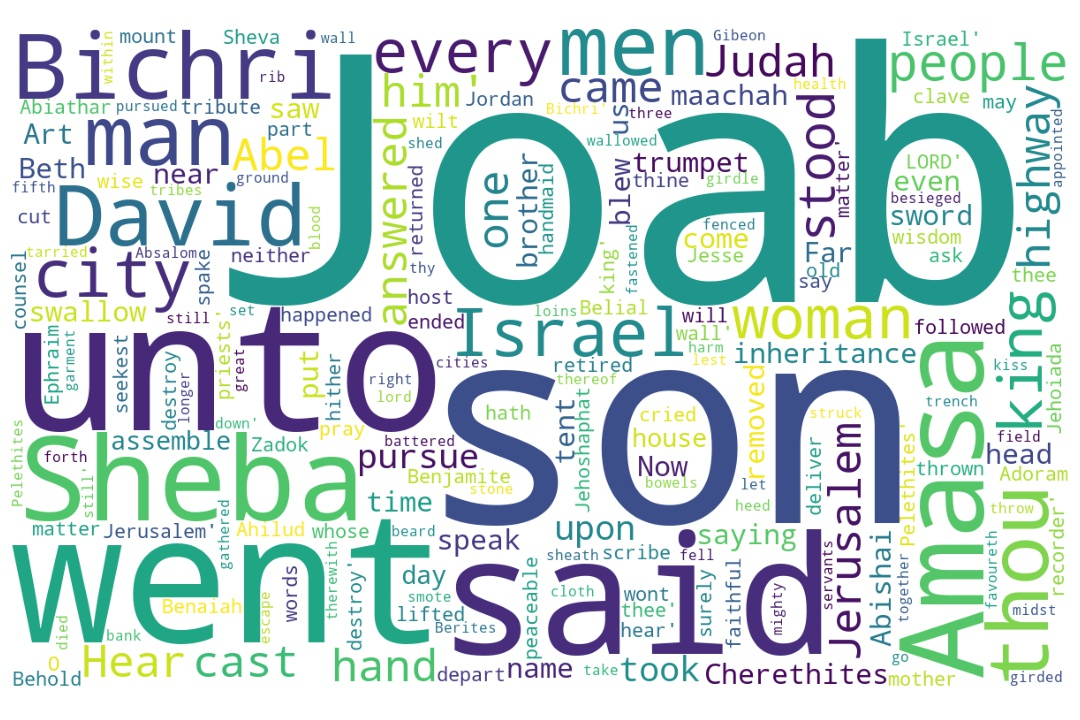
\includegraphics[width=\linewidth]{10OT-2Samuel/2Samuel20-WordCloud.jpg}
  \caption{1 Samuel 20 Word Cloud}
  \label{fig:1 Samuel 20 Word Cloud}
\end{figure}

%%%%%%%%%%%%%%%%%%%%%%%%%%%%%%%%%%%%%%%%%
%%%%%%%%%%%%%%%%%%%%%%%%%%%%%%%%%%%%%%%%%

\marginpar{\scriptsize \centering \fcolorbox{bone}{lime}{\textbf{CONFLICT \& CHARACTER}}\\ (2 Samuel 20:1-26) \begin{compactenum}[I.][8]
   \item The  \textbf{Next} Revolt \index[scripture]{2Samuel!2Sa 20:01} (2Sa 20:1) 
   \item The  \textbf{Northern} Hostility \index[scripture]{2Samuel!2Sa 20:02} (2Sa 20:2) 
   \item A  \textbf{Nasty} Ambush \index[scripture]{2Samuel!2Sa 20:10} (2Sa 20:10) 
   \item A  \textbf{Narrow} Mind \index[scripture]{2Samuel!2Sa 20:11} (2Sa 20:11) 
   \item A  \textbf{Necessary} Judgment \index[scripture]{2Samuel!2Sa 20:22} (2Sa 20:22) 
   \item  \textbf{Named} Officials \index[scripture]{2Samuel!2Sa 20:23--26} (2Sa 20:23--26) 
   \item A  \textbf{Notable} Contradiction -- David's disdain for men like Joab, yet dependence on them (see \index[scripture]{2Samuel!2Sa 19:22} 2Sa 19:22) 
\end{compactenum}}

\footnote{\textcolor[cmyk]{0.99998,1,0,0}{\hyperlink{TOC}{Return to end of Table of Contents.}}}\footnote{\href{https://audiobible.com/bible/2_samuel_20.html}{\textcolor[cmyk]{0.99998,1,0,0}{2 Samuel 20 Audio}}}\textcolor[cmyk]{0.99998,1,0,0}{And there happened to be there \fcolorbox{bone}{bone}{a} man of Belial, whose name \emph{was} Sheba, the son of Bichri, \fcolorbox{bone}{bone}{a} Benjamite: and he blew \fcolorbox{bone}{bone}{a} trumpet, and said, We have \fcolorbox{bone}{lime}{no part in David}, neither have we inheritance in the son of Jesse: every man to his tents, O Israel.}
[2] \textcolor[cmyk]{0.99998,1,0,0}{So every man of Israel went up from after David, \emph{and} \fcolorbox{bone}{lime}{followed Sheba} the son of Bichri: but the men of Judah clave unto their king, from Jordan even to Jerusalem.}\\
\\
\P \textcolor[cmyk]{0.99998,1,0,0}{And David came to his house at Jerusalem; and the king took the ten women \emph{his} concubines, whom he had left to keep the house, and put them in ward, and fed them, but went not in unto them. So they were shut up unto the day of their death, living in widowhood.}\\
\\
\P \textcolor[cmyk]{0.99998,1,0,0}{Then said the king to Amasa, Assemble me the men of Judah within three days, and be thou here present.}
[5] \textcolor[cmyk]{0.99998,1,0,0}{So Amasa went to assemble \emph{the} \emph{men} \emph{of} Judah: but he tarried longer than the set time which he had appointed him.}
[6] \textcolor[cmyk]{0.99998,1,0,0}{And David said to Abishai, Now shall Sheba the son of Bichri do us more harm than \emph{did} Absalom: take thou thy lord's servants, and pursue after him, lest he get him fenced cities, and escape us.}
[7] \textcolor[cmyk]{0.99998,1,0,0}{And there went out after him Joab's men, and the Cherethites, and the Pelethites, and all the mighty men: and they went out of Jerusalem, to pursue after Sheba the son of Bichri.}
[8] \textcolor[cmyk]{0.99998,1,0,0}{When they \emph{were} at the great stone which \emph{is} in Gibeon, Amasa went before them. And Joab's garment that he had put on was girded unto him, and upon it \fcolorbox{bone}{bone}{a} girdle \emph{with} \fcolorbox{bone}{bone}{a} sword fastened upon his loins in the sheath thereof; and as he went forth it fell out.}
[9] \textcolor[cmyk]{0.99998,1,0,0}{And Joab said to Amasa, \emph{Art} thou in health, my brother? And Joab took Amasa by the beard with the right hand to kiss him.}
[10] \textcolor[cmyk]{0.99998,1,0,0}{But Amasa took no heed to the sword that \emph{was} in Joab's hand: so he \fcolorbox{bone}{lime}{smote him} therewith in the fifth \emph{rib}, and shed out his bowels to the ground, and struck him not again; and he died. So Joab and Abishai his brother pursued after Sheba the son of Bichri.}
[11] \textcolor[cmyk]{0.99998,1,0,0}{And one of Joab's men stood by him, and said, He that favoureth Joab, and he that \emph{is} for David, \emph{let} \emph{him} \fcolorbox{bone}{lime}{\emph{go} after Joab}.}
[12] \textcolor[cmyk]{0.99998,1,0,0}{And Amasa wallowed in blood in the midst of the highway. And when the man saw that all the people stood still, he removed Amasa out of the highway into the field, and cast \fcolorbox{bone}{bone}{a} cloth upon him, when he saw that every one that came by him stood still.}
[13] \textcolor[cmyk]{0.99998,1,0,0}{When he was removed out of the highway, all the people went on after Joab, to pursue after Sheba the son of Bichri.}\\
\\
\P \textcolor[cmyk]{0.99998,1,0,0}{And he went through all the tribes of Israel unto Abel, and to Beth-maachah, and all the Berites: and they were gathered together, and went also after him.}
[15] \textcolor[cmyk]{0.99998,1,0,0}{And they came and besieged him in Abel of Beth-maachah, and they cast up \fcolorbox{bone}{bone}{a} bank against the city, and it stood in the trench: and all the people that \emph{were} with Joab battered the wall, to throw it down.}\\
\\
\P \textcolor[cmyk]{0.99998,1,0,0}{Then cried \fcolorbox{bone}{bone}{a} wise woman out of the city, Hear, hear; say, I pray you, unto Joab, Come near hither, that I may speak with thee.}
[17] \textcolor[cmyk]{0.99998,1,0,0}{And when he was come near unto her, the woman said, \emph{Art} thou Joab? And he answered, I \emph{am} \emph{he}. Then she said unto him, Hear the words of thine handmaid. And he answered, I do hear.}
[18] \textcolor[cmyk]{0.99998,1,0,0}{Then she spake, saying, They were wont to speak in old time, saying, They shall surely ask \emph{counsel} at Abel: and so they ended \emph{the} \emph{matter}.}
[19] \textcolor[cmyk]{0.99998,1,0,0}{I \emph{am} \emph{one} \emph{of} \emph{them} \emph{that} \emph{are} peaceable \emph{and} faithful in Israel: thou seekest to destroy \fcolorbox{bone}{bone}{a} city and \fcolorbox{bone}{bone}{a} mother in Israel: why wilt thou swallow up the inheritance of the LORD?}
[20] \textcolor[cmyk]{0.99998,1,0,0}{And Joab answered and said, Far be it, far be it from me, that I should swallow up or destroy.}
[21] \textcolor[cmyk]{0.99998,1,0,0}{The matter \emph{is} not so: but \fcolorbox{bone}{bone}{a} man of mount Ephraim, Sheba the son of Bichri by name, hath lifted up his hand against the king, \emph{even} against David: deliver him only, and I will depart from the city. And the woman said unto Joab, Behold, his head shall be thrown to thee over the wall.}
[22] \textcolor[cmyk]{0.99998,1,0,0}{Then the woman went unto all the people in her wisdom. And they \fcolorbox{bone}{lime}{cut off the head} of Sheba the son of Bichri, and cast \emph{it} out to Joab. And he blew \fcolorbox{bone}{bone}{a} trumpet, and they retired from the city, every man to his tent. And Joab returned to Jerusalem unto the king.}\\
\\
\P \textcolor[cmyk]{0.99998,1,0,0}{Now \fcolorbox{bone}{lime}{Joab} \emph{was} over all the host of Israel: and \fcolorbox{bone}{lime}{Benaiah} the son of Jehoiada \emph{was} over the Cherethites and over the Pelethites:}
[24] \textcolor[cmyk]{0.99998,1,0,0}{And \fcolorbox{bone}{lime}{Adoram} \emph{was} over the tribute: and Jehoshaphat the son of Ahilud \emph{was} recorder:}
[25] \textcolor[cmyk]{0.99998,1,0,0}{And \fcolorbox{bone}{lime}{Sheva} \emph{was} scribe: and \fcolorbox{bone}{lime}{Zadok} and \fcolorbox{bone}{lime}{Abiathar} \emph{were} the priests:}
[26] \textcolor[cmyk]{0.99998,1,0,0}{And \fcolorbox{bone}{lime}{Ira} also the Jairite was \fcolorbox{bone}{bone}{a} chief ruler about David.}
\index[NWIV]{49!2Samuel!2Sa 20:1}\index[AWIP]{And!2Samuel!2Sa 20:1}\index[AWIP]{there!2Samuel!2Sa 20:1}\index[AWIP]{there!2Samuel!2Sa 20:1 (2)}\index[AWIP]{happened!2Samuel!2Sa 20:1}\index[AWIP]{to!2Samuel!2Sa 20:1}\index[AWIP]{to!2Samuel!2Sa 20:1 (2)}\index[AWIP]{be!2Samuel!2Sa 20:1}\index[AWIP]{a!2Samuel!2Sa 20:1}\index[AWIP]{a!2Samuel!2Sa 20:1 (2)}\index[AWIP]{a!2Samuel!2Sa 20:1 (3)}\index[AWIP]{man!2Samuel!2Sa 20:1}\index[AWIP]{man!2Samuel!2Sa 20:1 (2)}\index[AWIP]{of!2Samuel!2Sa 20:1}\index[AWIP]{of!2Samuel!2Sa 20:1 (2)}\index[AWIP]{of!2Samuel!2Sa 20:1 (3)}\index[AWIP]{Belial!2Samuel!2Sa 20:1}\index[AWIP]{whose!2Samuel!2Sa 20:1}\index[AWIP]{name!2Samuel!2Sa 20:1}\index[AWIP]{\emph{was}!2Samuel!2Sa 20:1}\index[AWIP]{Sheba!2Samuel!2Sa 20:1}\index[AWIP]{the!2Samuel!2Sa 20:1}\index[AWIP]{the!2Samuel!2Sa 20:1 (2)}\index[AWIP]{son!2Samuel!2Sa 20:1}\index[AWIP]{son!2Samuel!2Sa 20:1 (2)}\index[AWIP]{Bichri!2Samuel!2Sa 20:1}\index[AWIP]{Benjamite!2Samuel!2Sa 20:1}\index[AWIP]{and!2Samuel!2Sa 20:1}\index[AWIP]{and!2Samuel!2Sa 20:1 (2)}\index[AWIP]{he!2Samuel!2Sa 20:1}\index[AWIP]{blew!2Samuel!2Sa 20:1}\index[AWIP]{trumpet!2Samuel!2Sa 20:1}\index[AWIP]{said!2Samuel!2Sa 20:1}\index[AWIP]{We!2Samuel!2Sa 20:1}\index[AWIP]{have!2Samuel!2Sa 20:1}\index[AWIP]{have!2Samuel!2Sa 20:1 (2)}\index[AWIP]{no!2Samuel!2Sa 20:1}\index[AWIP]{part!2Samuel!2Sa 20:1}\index[AWIP]{in!2Samuel!2Sa 20:1}\index[AWIP]{in!2Samuel!2Sa 20:1 (2)}\index[AWIP]{David!2Samuel!2Sa 20:1}\index[AWIP]{neither!2Samuel!2Sa 20:1}\index[AWIP]{we!2Samuel!2Sa 20:1}\index[AWIP]{inheritance!2Samuel!2Sa 20:1}\index[AWIP]{Jesse!2Samuel!2Sa 20:1}\index[AWIP]{every!2Samuel!2Sa 20:1}\index[AWIP]{his!2Samuel!2Sa 20:1}\index[AWIP]{tents!2Samuel!2Sa 20:1}\index[AWIP]{O!2Samuel!2Sa 20:1}\index[AWIP]{Israel!2Samuel!2Sa 20:1}\index[AWIP]{\emph{was}!2Samuel!2Sa 20:1}

\index[NWIV]{31!2Samuel!2Sa 20:2}\index[AWIP]{So!2Samuel!2Sa 20:2}\index[AWIP]{every!2Samuel!2Sa 20:2}\index[AWIP]{man!2Samuel!2Sa 20:2}\index[AWIP]{of!2Samuel!2Sa 20:2}\index[AWIP]{of!2Samuel!2Sa 20:2 (2)}\index[AWIP]{of!2Samuel!2Sa 20:2 (3)}\index[AWIP]{Israel!2Samuel!2Sa 20:2}\index[AWIP]{went!2Samuel!2Sa 20:2}\index[AWIP]{up!2Samuel!2Sa 20:2}\index[AWIP]{from!2Samuel!2Sa 20:2}\index[AWIP]{from!2Samuel!2Sa 20:2 (2)}\index[AWIP]{after!2Samuel!2Sa 20:2}\index[AWIP]{David!2Samuel!2Sa 20:2}\index[AWIP]{\emph{and}!2Samuel!2Sa 20:2}\index[AWIP]{followed!2Samuel!2Sa 20:2}\index[AWIP]{Sheba!2Samuel!2Sa 20:2}\index[AWIP]{the!2Samuel!2Sa 20:2}\index[AWIP]{the!2Samuel!2Sa 20:2 (2)}\index[AWIP]{son!2Samuel!2Sa 20:2}\index[AWIP]{Bichri!2Samuel!2Sa 20:2}\index[AWIP]{but!2Samuel!2Sa 20:2}\index[AWIP]{men!2Samuel!2Sa 20:2}\index[AWIP]{Judah!2Samuel!2Sa 20:2}\index[AWIP]{clave!2Samuel!2Sa 20:2}\index[AWIP]{unto!2Samuel!2Sa 20:2}\index[AWIP]{their!2Samuel!2Sa 20:2}\index[AWIP]{king!2Samuel!2Sa 20:2}\index[AWIP]{Jordan!2Samuel!2Sa 20:2}\index[AWIP]{even!2Samuel!2Sa 20:2}\index[AWIP]{to!2Samuel!2Sa 20:2}\index[AWIP]{Jerusalem!2Samuel!2Sa 20:2}\index[AWIP]{\emph{and}!2Samuel!2Sa 20:2}

\index[NWIV]{53!2Samuel!2Sa 20:3}\index[AWIP]{And!2Samuel!2Sa 20:3}\index[AWIP]{David!2Samuel!2Sa 20:3}\index[AWIP]{came!2Samuel!2Sa 20:3}\index[AWIP]{to!2Samuel!2Sa 20:3}\index[AWIP]{to!2Samuel!2Sa 20:3 (2)}\index[AWIP]{his!2Samuel!2Sa 20:3}\index[AWIP]{house!2Samuel!2Sa 20:3}\index[AWIP]{house!2Samuel!2Sa 20:3 (2)}\index[AWIP]{at!2Samuel!2Sa 20:3}\index[AWIP]{Jerusalem!2Samuel!2Sa 20:3}\index[AWIP]{and!2Samuel!2Sa 20:3}\index[AWIP]{and!2Samuel!2Sa 20:3 (2)}\index[AWIP]{and!2Samuel!2Sa 20:3 (3)}\index[AWIP]{the!2Samuel!2Sa 20:3}\index[AWIP]{the!2Samuel!2Sa 20:3 (2)}\index[AWIP]{the!2Samuel!2Sa 20:3 (3)}\index[AWIP]{the!2Samuel!2Sa 20:3 (4)}\index[AWIP]{king!2Samuel!2Sa 20:3}\index[AWIP]{took!2Samuel!2Sa 20:3}\index[AWIP]{ten!2Samuel!2Sa 20:3}\index[AWIP]{women!2Samuel!2Sa 20:3}\index[AWIP]{\emph{his}!2Samuel!2Sa 20:3}\index[AWIP]{concubines!2Samuel!2Sa 20:3}\index[AWIP]{whom!2Samuel!2Sa 20:3}\index[AWIP]{he!2Samuel!2Sa 20:3}\index[AWIP]{had!2Samuel!2Sa 20:3}\index[AWIP]{left!2Samuel!2Sa 20:3}\index[AWIP]{keep!2Samuel!2Sa 20:3}\index[AWIP]{put!2Samuel!2Sa 20:3}\index[AWIP]{them!2Samuel!2Sa 20:3}\index[AWIP]{them!2Samuel!2Sa 20:3 (2)}\index[AWIP]{them!2Samuel!2Sa 20:3 (3)}\index[AWIP]{in!2Samuel!2Sa 20:3}\index[AWIP]{in!2Samuel!2Sa 20:3 (2)}\index[AWIP]{in!2Samuel!2Sa 20:3 (3)}\index[AWIP]{ward!2Samuel!2Sa 20:3}\index[AWIP]{fed!2Samuel!2Sa 20:3}\index[AWIP]{but!2Samuel!2Sa 20:3}\index[AWIP]{went!2Samuel!2Sa 20:3}\index[AWIP]{not!2Samuel!2Sa 20:3}\index[AWIP]{unto!2Samuel!2Sa 20:3}\index[AWIP]{unto!2Samuel!2Sa 20:3 (2)}\index[AWIP]{So!2Samuel!2Sa 20:3}\index[AWIP]{they!2Samuel!2Sa 20:3}\index[AWIP]{were!2Samuel!2Sa 20:3}\index[AWIP]{shut!2Samuel!2Sa 20:3}\index[AWIP]{up!2Samuel!2Sa 20:3}\index[AWIP]{day!2Samuel!2Sa 20:3}\index[AWIP]{of!2Samuel!2Sa 20:3}\index[AWIP]{their!2Samuel!2Sa 20:3}\index[AWIP]{death!2Samuel!2Sa 20:3}\index[AWIP]{living!2Samuel!2Sa 20:3}\index[AWIP]{widowhood!2Samuel!2Sa 20:3}\index[AWIP]{\emph{his}!2Samuel!2Sa 20:3}

\index[NWIV]{20!2Samuel!2Sa 20:4}\index[AWIP]{Then!2Samuel!2Sa 20:4}\index[AWIP]{said!2Samuel!2Sa 20:4}\index[AWIP]{the!2Samuel!2Sa 20:4}\index[AWIP]{the!2Samuel!2Sa 20:4 (2)}\index[AWIP]{king!2Samuel!2Sa 20:4}\index[AWIP]{to!2Samuel!2Sa 20:4}\index[AWIP]{Amasa!2Samuel!2Sa 20:4}\index[AWIP]{Assemble!2Samuel!2Sa 20:4}\index[AWIP]{me!2Samuel!2Sa 20:4}\index[AWIP]{men!2Samuel!2Sa 20:4}\index[AWIP]{of!2Samuel!2Sa 20:4}\index[AWIP]{Judah!2Samuel!2Sa 20:4}\index[AWIP]{within!2Samuel!2Sa 20:4}\index[AWIP]{three!2Samuel!2Sa 20:4}\index[AWIP]{days!2Samuel!2Sa 20:4}\index[AWIP]{and!2Samuel!2Sa 20:4}\index[AWIP]{be!2Samuel!2Sa 20:4}\index[AWIP]{thou!2Samuel!2Sa 20:4}\index[AWIP]{here!2Samuel!2Sa 20:4}\index[AWIP]{present!2Samuel!2Sa 20:4}

\index[NWIV]{22!2Samuel!2Sa 20:5}\index[AWIP]{So!2Samuel!2Sa 20:5}\index[AWIP]{Amasa!2Samuel!2Sa 20:5}\index[AWIP]{went!2Samuel!2Sa 20:5}\index[AWIP]{to!2Samuel!2Sa 20:5}\index[AWIP]{assemble!2Samuel!2Sa 20:5}\index[AWIP]{\emph{the}!2Samuel!2Sa 20:5}\index[AWIP]{\emph{men}!2Samuel!2Sa 20:5}\index[AWIP]{\emph{of}!2Samuel!2Sa 20:5}\index[AWIP]{Judah!2Samuel!2Sa 20:5}\index[AWIP]{but!2Samuel!2Sa 20:5}\index[AWIP]{he!2Samuel!2Sa 20:5}\index[AWIP]{he!2Samuel!2Sa 20:5 (2)}\index[AWIP]{tarried!2Samuel!2Sa 20:5}\index[AWIP]{longer!2Samuel!2Sa 20:5}\index[AWIP]{than!2Samuel!2Sa 20:5}\index[AWIP]{the!2Samuel!2Sa 20:5}\index[AWIP]{set!2Samuel!2Sa 20:5}\index[AWIP]{time!2Samuel!2Sa 20:5}\index[AWIP]{which!2Samuel!2Sa 20:5}\index[AWIP]{had!2Samuel!2Sa 20:5}\index[AWIP]{appointed!2Samuel!2Sa 20:5}\index[AWIP]{him!2Samuel!2Sa 20:5}\index[AWIP]{\emph{the}!2Samuel!2Sa 20:5}\index[AWIP]{\emph{men}!2Samuel!2Sa 20:5}\index[AWIP]{\emph{of}!2Samuel!2Sa 20:5}

\index[NWIV]{37!2Samuel!2Sa 20:6}\index[AWIP]{And!2Samuel!2Sa 20:6}\index[AWIP]{David!2Samuel!2Sa 20:6}\index[AWIP]{said!2Samuel!2Sa 20:6}\index[AWIP]{to!2Samuel!2Sa 20:6}\index[AWIP]{Abishai!2Samuel!2Sa 20:6}\index[AWIP]{Now!2Samuel!2Sa 20:6}\index[AWIP]{shall!2Samuel!2Sa 20:6}\index[AWIP]{Sheba!2Samuel!2Sa 20:6}\index[AWIP]{the!2Samuel!2Sa 20:6}\index[AWIP]{son!2Samuel!2Sa 20:6}\index[AWIP]{of!2Samuel!2Sa 20:6}\index[AWIP]{Bichri!2Samuel!2Sa 20:6}\index[AWIP]{do!2Samuel!2Sa 20:6}\index[AWIP]{us!2Samuel!2Sa 20:6}\index[AWIP]{us!2Samuel!2Sa 20:6 (2)}\index[AWIP]{more!2Samuel!2Sa 20:6}\index[AWIP]{harm!2Samuel!2Sa 20:6}\index[AWIP]{than!2Samuel!2Sa 20:6}\index[AWIP]{\emph{did}!2Samuel!2Sa 20:6}\index[AWIP]{Absalom!2Samuel!2Sa 20:6}\index[AWIP]{take!2Samuel!2Sa 20:6}\index[AWIP]{thou!2Samuel!2Sa 20:6}\index[AWIP]{thy!2Samuel!2Sa 20:6}\index[AWIP]{lord's!2Samuel!2Sa 20:6}\index[AWIP]{servants!2Samuel!2Sa 20:6}\index[AWIP]{and!2Samuel!2Sa 20:6}\index[AWIP]{and!2Samuel!2Sa 20:6 (2)}\index[AWIP]{pursue!2Samuel!2Sa 20:6}\index[AWIP]{after!2Samuel!2Sa 20:6}\index[AWIP]{him!2Samuel!2Sa 20:6}\index[AWIP]{him!2Samuel!2Sa 20:6 (2)}\index[AWIP]{lest!2Samuel!2Sa 20:6}\index[AWIP]{he!2Samuel!2Sa 20:6}\index[AWIP]{get!2Samuel!2Sa 20:6}\index[AWIP]{fenced!2Samuel!2Sa 20:6}\index[AWIP]{cities!2Samuel!2Sa 20:6}\index[AWIP]{escape!2Samuel!2Sa 20:6}\index[AWIP]{\emph{did}!2Samuel!2Sa 20:6}

\index[NWIV]{33!2Samuel!2Sa 20:7}\index[AWIP]{And!2Samuel!2Sa 20:7}\index[AWIP]{there!2Samuel!2Sa 20:7}\index[AWIP]{went!2Samuel!2Sa 20:7}\index[AWIP]{went!2Samuel!2Sa 20:7 (2)}\index[AWIP]{out!2Samuel!2Sa 20:7}\index[AWIP]{out!2Samuel!2Sa 20:7 (2)}\index[AWIP]{after!2Samuel!2Sa 20:7}\index[AWIP]{after!2Samuel!2Sa 20:7 (2)}\index[AWIP]{him!2Samuel!2Sa 20:7}\index[AWIP]{Joab's!2Samuel!2Sa 20:7}\index[AWIP]{men!2Samuel!2Sa 20:7}\index[AWIP]{men!2Samuel!2Sa 20:7 (2)}\index[AWIP]{and!2Samuel!2Sa 20:7}\index[AWIP]{and!2Samuel!2Sa 20:7 (2)}\index[AWIP]{and!2Samuel!2Sa 20:7 (3)}\index[AWIP]{and!2Samuel!2Sa 20:7 (4)}\index[AWIP]{the!2Samuel!2Sa 20:7}\index[AWIP]{the!2Samuel!2Sa 20:7 (2)}\index[AWIP]{the!2Samuel!2Sa 20:7 (3)}\index[AWIP]{the!2Samuel!2Sa 20:7 (4)}\index[AWIP]{Cherethites!2Samuel!2Sa 20:7}\index[AWIP]{Pelethites!2Samuel!2Sa 20:7}\index[AWIP]{all!2Samuel!2Sa 20:7}\index[AWIP]{mighty!2Samuel!2Sa 20:7}\index[AWIP]{they!2Samuel!2Sa 20:7}\index[AWIP]{of!2Samuel!2Sa 20:7}\index[AWIP]{of!2Samuel!2Sa 20:7 (2)}\index[AWIP]{Jerusalem!2Samuel!2Sa 20:7}\index[AWIP]{to!2Samuel!2Sa 20:7}\index[AWIP]{pursue!2Samuel!2Sa 20:7}\index[AWIP]{Sheba!2Samuel!2Sa 20:7}\index[AWIP]{son!2Samuel!2Sa 20:7}\index[AWIP]{Bichri!2Samuel!2Sa 20:7}

\index[NWIV]{51!2Samuel!2Sa 20:8}\index[AWIP]{When!2Samuel!2Sa 20:8}\index[AWIP]{they!2Samuel!2Sa 20:8}\index[AWIP]{\emph{were}!2Samuel!2Sa 20:8}\index[AWIP]{at!2Samuel!2Sa 20:8}\index[AWIP]{the!2Samuel!2Sa 20:8}\index[AWIP]{the!2Samuel!2Sa 20:8 (2)}\index[AWIP]{great!2Samuel!2Sa 20:8}\index[AWIP]{stone!2Samuel!2Sa 20:8}\index[AWIP]{which!2Samuel!2Sa 20:8}\index[AWIP]{\emph{is}!2Samuel!2Sa 20:8}\index[AWIP]{in!2Samuel!2Sa 20:8}\index[AWIP]{in!2Samuel!2Sa 20:8 (2)}\index[AWIP]{Gibeon!2Samuel!2Sa 20:8}\index[AWIP]{Amasa!2Samuel!2Sa 20:8}\index[AWIP]{went!2Samuel!2Sa 20:8}\index[AWIP]{went!2Samuel!2Sa 20:8 (2)}\index[AWIP]{before!2Samuel!2Sa 20:8}\index[AWIP]{them!2Samuel!2Sa 20:8}\index[AWIP]{And!2Samuel!2Sa 20:8}\index[AWIP]{Joab's!2Samuel!2Sa 20:8}\index[AWIP]{garment!2Samuel!2Sa 20:8}\index[AWIP]{that!2Samuel!2Sa 20:8}\index[AWIP]{he!2Samuel!2Sa 20:8}\index[AWIP]{he!2Samuel!2Sa 20:8 (2)}\index[AWIP]{had!2Samuel!2Sa 20:8}\index[AWIP]{put!2Samuel!2Sa 20:8}\index[AWIP]{on!2Samuel!2Sa 20:8}\index[AWIP]{was!2Samuel!2Sa 20:8}\index[AWIP]{girded!2Samuel!2Sa 20:8}\index[AWIP]{unto!2Samuel!2Sa 20:8}\index[AWIP]{him!2Samuel!2Sa 20:8}\index[AWIP]{and!2Samuel!2Sa 20:8}\index[AWIP]{and!2Samuel!2Sa 20:8 (2)}\index[AWIP]{upon!2Samuel!2Sa 20:8}\index[AWIP]{upon!2Samuel!2Sa 20:8 (2)}\index[AWIP]{it!2Samuel!2Sa 20:8}\index[AWIP]{it!2Samuel!2Sa 20:8 (2)}\index[AWIP]{a!2Samuel!2Sa 20:8}\index[AWIP]{a!2Samuel!2Sa 20:8 (2)}\index[AWIP]{girdle!2Samuel!2Sa 20:8}\index[AWIP]{\emph{with}!2Samuel!2Sa 20:8}\index[AWIP]{sword!2Samuel!2Sa 20:8}\index[AWIP]{fastened!2Samuel!2Sa 20:8}\index[AWIP]{his!2Samuel!2Sa 20:8}\index[AWIP]{loins!2Samuel!2Sa 20:8}\index[AWIP]{sheath!2Samuel!2Sa 20:8}\index[AWIP]{thereof!2Samuel!2Sa 20:8}\index[AWIP]{as!2Samuel!2Sa 20:8}\index[AWIP]{forth!2Samuel!2Sa 20:8}\index[AWIP]{fell!2Samuel!2Sa 20:8}\index[AWIP]{out!2Samuel!2Sa 20:8}\index[AWIP]{\emph{were}!2Samuel!2Sa 20:8}\index[AWIP]{\emph{is}!2Samuel!2Sa 20:8}\index[AWIP]{\emph{with}!2Samuel!2Sa 20:8}

\index[NWIV]{25!2Samuel!2Sa 20:9}\index[AWIP]{And!2Samuel!2Sa 20:9}\index[AWIP]{And!2Samuel!2Sa 20:9 (2)}\index[AWIP]{Joab!2Samuel!2Sa 20:9}\index[AWIP]{Joab!2Samuel!2Sa 20:9 (2)}\index[AWIP]{said!2Samuel!2Sa 20:9}\index[AWIP]{to!2Samuel!2Sa 20:9}\index[AWIP]{to!2Samuel!2Sa 20:9 (2)}\index[AWIP]{Amasa!2Samuel!2Sa 20:9}\index[AWIP]{Amasa!2Samuel!2Sa 20:9 (2)}\index[AWIP]{\emph{Art}!2Samuel!2Sa 20:9}\index[AWIP]{thou!2Samuel!2Sa 20:9}\index[AWIP]{in!2Samuel!2Sa 20:9}\index[AWIP]{health!2Samuel!2Sa 20:9}\index[AWIP]{my!2Samuel!2Sa 20:9}\index[AWIP]{brother?!2Samuel!2Sa 20:9}\index[AWIP]{took!2Samuel!2Sa 20:9}\index[AWIP]{by!2Samuel!2Sa 20:9}\index[AWIP]{the!2Samuel!2Sa 20:9}\index[AWIP]{the!2Samuel!2Sa 20:9 (2)}\index[AWIP]{beard!2Samuel!2Sa 20:9}\index[AWIP]{with!2Samuel!2Sa 20:9}\index[AWIP]{right!2Samuel!2Sa 20:9}\index[AWIP]{hand!2Samuel!2Sa 20:9}\index[AWIP]{kiss!2Samuel!2Sa 20:9}\index[AWIP]{him!2Samuel!2Sa 20:9}\index[AWIP]{\emph{Art}!2Samuel!2Sa 20:9}

\index[NWIV]{51!2Samuel!2Sa 20:10}\index[AWIP]{But!2Samuel!2Sa 20:10}\index[AWIP]{Amasa!2Samuel!2Sa 20:10}\index[AWIP]{took!2Samuel!2Sa 20:10}\index[AWIP]{no!2Samuel!2Sa 20:10}\index[AWIP]{heed!2Samuel!2Sa 20:10}\index[AWIP]{to!2Samuel!2Sa 20:10}\index[AWIP]{to!2Samuel!2Sa 20:10 (2)}\index[AWIP]{the!2Samuel!2Sa 20:10}\index[AWIP]{the!2Samuel!2Sa 20:10 (2)}\index[AWIP]{the!2Samuel!2Sa 20:10 (3)}\index[AWIP]{the!2Samuel!2Sa 20:10 (4)}\index[AWIP]{sword!2Samuel!2Sa 20:10}\index[AWIP]{that!2Samuel!2Sa 20:10}\index[AWIP]{\emph{was}!2Samuel!2Sa 20:10}\index[AWIP]{in!2Samuel!2Sa 20:10}\index[AWIP]{in!2Samuel!2Sa 20:10 (2)}\index[AWIP]{Joab's!2Samuel!2Sa 20:10}\index[AWIP]{hand!2Samuel!2Sa 20:10}\index[AWIP]{so!2Samuel!2Sa 20:10}\index[AWIP]{he!2Samuel!2Sa 20:10}\index[AWIP]{he!2Samuel!2Sa 20:10 (2)}\index[AWIP]{smote!2Samuel!2Sa 20:10}\index[AWIP]{him!2Samuel!2Sa 20:10}\index[AWIP]{him!2Samuel!2Sa 20:10 (2)}\index[AWIP]{therewith!2Samuel!2Sa 20:10}\index[AWIP]{fifth!2Samuel!2Sa 20:10}\index[AWIP]{\emph{rib}!2Samuel!2Sa 20:10}\index[AWIP]{and!2Samuel!2Sa 20:10}\index[AWIP]{and!2Samuel!2Sa 20:10 (2)}\index[AWIP]{and!2Samuel!2Sa 20:10 (3)}\index[AWIP]{and!2Samuel!2Sa 20:10 (4)}\index[AWIP]{shed!2Samuel!2Sa 20:10}\index[AWIP]{out!2Samuel!2Sa 20:10}\index[AWIP]{his!2Samuel!2Sa 20:10}\index[AWIP]{his!2Samuel!2Sa 20:10 (2)}\index[AWIP]{bowels!2Samuel!2Sa 20:10}\index[AWIP]{ground!2Samuel!2Sa 20:10}\index[AWIP]{struck!2Samuel!2Sa 20:10}\index[AWIP]{not!2Samuel!2Sa 20:10}\index[AWIP]{again!2Samuel!2Sa 20:10}\index[AWIP]{died!2Samuel!2Sa 20:10}\index[AWIP]{So!2Samuel!2Sa 20:10}\index[AWIP]{Joab!2Samuel!2Sa 20:10}\index[AWIP]{Abishai!2Samuel!2Sa 20:10}\index[AWIP]{brother!2Samuel!2Sa 20:10}\index[AWIP]{pursued!2Samuel!2Sa 20:10}\index[AWIP]{after!2Samuel!2Sa 20:10}\index[AWIP]{Sheba!2Samuel!2Sa 20:10}\index[AWIP]{son!2Samuel!2Sa 20:10}\index[AWIP]{of!2Samuel!2Sa 20:10}\index[AWIP]{Bichri!2Samuel!2Sa 20:10}\index[AWIP]{\emph{was}!2Samuel!2Sa 20:10}\index[AWIP]{\emph{rib}!2Samuel!2Sa 20:10}

\index[NWIV]{25!2Samuel!2Sa 20:11}\index[AWIP]{And!2Samuel!2Sa 20:11}\index[AWIP]{one!2Samuel!2Sa 20:11}\index[AWIP]{of!2Samuel!2Sa 20:11}\index[AWIP]{Joab's!2Samuel!2Sa 20:11}\index[AWIP]{men!2Samuel!2Sa 20:11}\index[AWIP]{stood!2Samuel!2Sa 20:11}\index[AWIP]{by!2Samuel!2Sa 20:11}\index[AWIP]{him!2Samuel!2Sa 20:11}\index[AWIP]{and!2Samuel!2Sa 20:11}\index[AWIP]{and!2Samuel!2Sa 20:11 (2)}\index[AWIP]{said!2Samuel!2Sa 20:11}\index[AWIP]{He!2Samuel!2Sa 20:11}\index[AWIP]{that!2Samuel!2Sa 20:11}\index[AWIP]{that!2Samuel!2Sa 20:11 (2)}\index[AWIP]{favoureth!2Samuel!2Sa 20:11}\index[AWIP]{Joab!2Samuel!2Sa 20:11}\index[AWIP]{Joab!2Samuel!2Sa 20:11 (2)}\index[AWIP]{he!2Samuel!2Sa 20:11}\index[AWIP]{\emph{is}!2Samuel!2Sa 20:11}\index[AWIP]{for!2Samuel!2Sa 20:11}\index[AWIP]{David!2Samuel!2Sa 20:11}\index[AWIP]{\emph{let}!2Samuel!2Sa 20:11}\index[AWIP]{\emph{him}!2Samuel!2Sa 20:11}\index[AWIP]{\emph{go}!2Samuel!2Sa 20:11}\index[AWIP]{after!2Samuel!2Sa 20:11}\index[AWIP]{\emph{is}!2Samuel!2Sa 20:11}\index[AWIP]{\emph{let}!2Samuel!2Sa 20:11}\index[AWIP]{\emph{him}!2Samuel!2Sa 20:11}\index[AWIP]{\emph{go}!2Samuel!2Sa 20:11}

\index[NWIV]{50!2Samuel!2Sa 20:12}\index[AWIP]{And!2Samuel!2Sa 20:12}\index[AWIP]{And!2Samuel!2Sa 20:12 (2)}\index[AWIP]{Amasa!2Samuel!2Sa 20:12}\index[AWIP]{Amasa!2Samuel!2Sa 20:12 (2)}\index[AWIP]{wallowed!2Samuel!2Sa 20:12}\index[AWIP]{in!2Samuel!2Sa 20:12}\index[AWIP]{in!2Samuel!2Sa 20:12 (2)}\index[AWIP]{blood!2Samuel!2Sa 20:12}\index[AWIP]{the!2Samuel!2Sa 20:12}\index[AWIP]{the!2Samuel!2Sa 20:12 (2)}\index[AWIP]{the!2Samuel!2Sa 20:12 (3)}\index[AWIP]{the!2Samuel!2Sa 20:12 (4)}\index[AWIP]{the!2Samuel!2Sa 20:12 (5)}\index[AWIP]{the!2Samuel!2Sa 20:12 (6)}\index[AWIP]{midst!2Samuel!2Sa 20:12}\index[AWIP]{of!2Samuel!2Sa 20:12}\index[AWIP]{of!2Samuel!2Sa 20:12 (2)}\index[AWIP]{highway!2Samuel!2Sa 20:12}\index[AWIP]{highway!2Samuel!2Sa 20:12 (2)}\index[AWIP]{when!2Samuel!2Sa 20:12}\index[AWIP]{when!2Samuel!2Sa 20:12 (2)}\index[AWIP]{man!2Samuel!2Sa 20:12}\index[AWIP]{saw!2Samuel!2Sa 20:12}\index[AWIP]{saw!2Samuel!2Sa 20:12 (2)}\index[AWIP]{that!2Samuel!2Sa 20:12}\index[AWIP]{that!2Samuel!2Sa 20:12 (2)}\index[AWIP]{that!2Samuel!2Sa 20:12 (3)}\index[AWIP]{all!2Samuel!2Sa 20:12}\index[AWIP]{people!2Samuel!2Sa 20:12}\index[AWIP]{stood!2Samuel!2Sa 20:12}\index[AWIP]{stood!2Samuel!2Sa 20:12 (2)}\index[AWIP]{still!2Samuel!2Sa 20:12}\index[AWIP]{still!2Samuel!2Sa 20:12 (2)}\index[AWIP]{he!2Samuel!2Sa 20:12}\index[AWIP]{he!2Samuel!2Sa 20:12 (2)}\index[AWIP]{removed!2Samuel!2Sa 20:12}\index[AWIP]{out!2Samuel!2Sa 20:12}\index[AWIP]{into!2Samuel!2Sa 20:12}\index[AWIP]{field!2Samuel!2Sa 20:12}\index[AWIP]{and!2Samuel!2Sa 20:12}\index[AWIP]{cast!2Samuel!2Sa 20:12}\index[AWIP]{a!2Samuel!2Sa 20:12}\index[AWIP]{cloth!2Samuel!2Sa 20:12}\index[AWIP]{upon!2Samuel!2Sa 20:12}\index[AWIP]{him!2Samuel!2Sa 20:12}\index[AWIP]{him!2Samuel!2Sa 20:12 (2)}\index[AWIP]{every!2Samuel!2Sa 20:12}\index[AWIP]{one!2Samuel!2Sa 20:12}\index[AWIP]{came!2Samuel!2Sa 20:12}\index[AWIP]{by!2Samuel!2Sa 20:12}

\index[NWIV]{23!2Samuel!2Sa 20:13}\index[AWIP]{When!2Samuel!2Sa 20:13}\index[AWIP]{he!2Samuel!2Sa 20:13}\index[AWIP]{was!2Samuel!2Sa 20:13}\index[AWIP]{removed!2Samuel!2Sa 20:13}\index[AWIP]{out!2Samuel!2Sa 20:13}\index[AWIP]{of!2Samuel!2Sa 20:13}\index[AWIP]{of!2Samuel!2Sa 20:13 (2)}\index[AWIP]{the!2Samuel!2Sa 20:13}\index[AWIP]{the!2Samuel!2Sa 20:13 (2)}\index[AWIP]{the!2Samuel!2Sa 20:13 (3)}\index[AWIP]{highway!2Samuel!2Sa 20:13}\index[AWIP]{all!2Samuel!2Sa 20:13}\index[AWIP]{people!2Samuel!2Sa 20:13}\index[AWIP]{went!2Samuel!2Sa 20:13}\index[AWIP]{on!2Samuel!2Sa 20:13}\index[AWIP]{after!2Samuel!2Sa 20:13}\index[AWIP]{after!2Samuel!2Sa 20:13 (2)}\index[AWIP]{Joab!2Samuel!2Sa 20:13}\index[AWIP]{to!2Samuel!2Sa 20:13}\index[AWIP]{pursue!2Samuel!2Sa 20:13}\index[AWIP]{Sheba!2Samuel!2Sa 20:13}\index[AWIP]{son!2Samuel!2Sa 20:13}\index[AWIP]{Bichri!2Samuel!2Sa 20:13}

\index[NWIV]{28!2Samuel!2Sa 20:14}\index[AWIP]{And!2Samuel!2Sa 20:14}\index[AWIP]{he!2Samuel!2Sa 20:14}\index[AWIP]{went!2Samuel!2Sa 20:14}\index[AWIP]{went!2Samuel!2Sa 20:14 (2)}\index[AWIP]{through!2Samuel!2Sa 20:14}\index[AWIP]{all!2Samuel!2Sa 20:14}\index[AWIP]{all!2Samuel!2Sa 20:14 (2)}\index[AWIP]{the!2Samuel!2Sa 20:14}\index[AWIP]{the!2Samuel!2Sa 20:14 (2)}\index[AWIP]{tribes!2Samuel!2Sa 20:14}\index[AWIP]{of!2Samuel!2Sa 20:14}\index[AWIP]{Israel!2Samuel!2Sa 20:14}\index[AWIP]{unto!2Samuel!2Sa 20:14}\index[AWIP]{Abel!2Samuel!2Sa 20:14}\index[AWIP]{and!2Samuel!2Sa 20:14}\index[AWIP]{and!2Samuel!2Sa 20:14 (2)}\index[AWIP]{and!2Samuel!2Sa 20:14 (3)}\index[AWIP]{and!2Samuel!2Sa 20:14 (4)}\index[AWIP]{to!2Samuel!2Sa 20:14}\index[AWIP]{Beth-maachah!2Samuel!2Sa 20:14}\index[AWIP]{Berites!2Samuel!2Sa 20:14}\index[AWIP]{they!2Samuel!2Sa 20:14}\index[AWIP]{were!2Samuel!2Sa 20:14}\index[AWIP]{gathered!2Samuel!2Sa 20:14}\index[AWIP]{together!2Samuel!2Sa 20:14}\index[AWIP]{also!2Samuel!2Sa 20:14}\index[AWIP]{after!2Samuel!2Sa 20:14}\index[AWIP]{him!2Samuel!2Sa 20:14}

\index[NWIV]{40!2Samuel!2Sa 20:15}\index[AWIP]{And!2Samuel!2Sa 20:15}\index[AWIP]{they!2Samuel!2Sa 20:15}\index[AWIP]{they!2Samuel!2Sa 20:15 (2)}\index[AWIP]{came!2Samuel!2Sa 20:15}\index[AWIP]{and!2Samuel!2Sa 20:15}\index[AWIP]{and!2Samuel!2Sa 20:15 (2)}\index[AWIP]{and!2Samuel!2Sa 20:15 (3)}\index[AWIP]{and!2Samuel!2Sa 20:15 (4)}\index[AWIP]{besieged!2Samuel!2Sa 20:15}\index[AWIP]{him!2Samuel!2Sa 20:15}\index[AWIP]{in!2Samuel!2Sa 20:15}\index[AWIP]{in!2Samuel!2Sa 20:15 (2)}\index[AWIP]{Abel!2Samuel!2Sa 20:15}\index[AWIP]{of!2Samuel!2Sa 20:15}\index[AWIP]{Beth-maachah!2Samuel!2Sa 20:15}\index[AWIP]{cast!2Samuel!2Sa 20:15}\index[AWIP]{up!2Samuel!2Sa 20:15}\index[AWIP]{a!2Samuel!2Sa 20:15}\index[AWIP]{bank!2Samuel!2Sa 20:15}\index[AWIP]{against!2Samuel!2Sa 20:15}\index[AWIP]{the!2Samuel!2Sa 20:15}\index[AWIP]{the!2Samuel!2Sa 20:15 (2)}\index[AWIP]{the!2Samuel!2Sa 20:15 (3)}\index[AWIP]{the!2Samuel!2Sa 20:15 (4)}\index[AWIP]{city!2Samuel!2Sa 20:15}\index[AWIP]{it!2Samuel!2Sa 20:15}\index[AWIP]{it!2Samuel!2Sa 20:15 (2)}\index[AWIP]{stood!2Samuel!2Sa 20:15}\index[AWIP]{trench!2Samuel!2Sa 20:15}\index[AWIP]{all!2Samuel!2Sa 20:15}\index[AWIP]{people!2Samuel!2Sa 20:15}\index[AWIP]{that!2Samuel!2Sa 20:15}\index[AWIP]{\emph{were}!2Samuel!2Sa 20:15}\index[AWIP]{with!2Samuel!2Sa 20:15}\index[AWIP]{Joab!2Samuel!2Sa 20:15}\index[AWIP]{battered!2Samuel!2Sa 20:15}\index[AWIP]{wall!2Samuel!2Sa 20:15}\index[AWIP]{to!2Samuel!2Sa 20:15}\index[AWIP]{throw!2Samuel!2Sa 20:15}\index[AWIP]{down!2Samuel!2Sa 20:15}\index[AWIP]{\emph{were}!2Samuel!2Sa 20:15}

\index[NWIV]{26!2Samuel!2Sa 20:16}\index[AWIP]{Then!2Samuel!2Sa 20:16}\index[AWIP]{cried!2Samuel!2Sa 20:16}\index[AWIP]{a!2Samuel!2Sa 20:16}\index[AWIP]{wise!2Samuel!2Sa 20:16}\index[AWIP]{woman!2Samuel!2Sa 20:16}\index[AWIP]{out!2Samuel!2Sa 20:16}\index[AWIP]{of!2Samuel!2Sa 20:16}\index[AWIP]{the!2Samuel!2Sa 20:16}\index[AWIP]{city!2Samuel!2Sa 20:16}\index[AWIP]{Hear!2Samuel!2Sa 20:16}\index[AWIP]{hear!2Samuel!2Sa 20:16}\index[AWIP]{say!2Samuel!2Sa 20:16}\index[AWIP]{I!2Samuel!2Sa 20:16}\index[AWIP]{I!2Samuel!2Sa 20:16 (2)}\index[AWIP]{pray!2Samuel!2Sa 20:16}\index[AWIP]{you!2Samuel!2Sa 20:16}\index[AWIP]{unto!2Samuel!2Sa 20:16}\index[AWIP]{Joab!2Samuel!2Sa 20:16}\index[AWIP]{Come!2Samuel!2Sa 20:16}\index[AWIP]{near!2Samuel!2Sa 20:16}\index[AWIP]{hither!2Samuel!2Sa 20:16}\index[AWIP]{that!2Samuel!2Sa 20:16}\index[AWIP]{may!2Samuel!2Sa 20:16}\index[AWIP]{speak!2Samuel!2Sa 20:16}\index[AWIP]{with!2Samuel!2Sa 20:16}\index[AWIP]{thee!2Samuel!2Sa 20:16}

\index[NWIV]{37!2Samuel!2Sa 20:17}\index[AWIP]{And!2Samuel!2Sa 20:17}\index[AWIP]{And!2Samuel!2Sa 20:17 (2)}\index[AWIP]{And!2Samuel!2Sa 20:17 (3)}\index[AWIP]{when!2Samuel!2Sa 20:17}\index[AWIP]{he!2Samuel!2Sa 20:17}\index[AWIP]{he!2Samuel!2Sa 20:17 (2)}\index[AWIP]{he!2Samuel!2Sa 20:17 (3)}\index[AWIP]{was!2Samuel!2Sa 20:17}\index[AWIP]{come!2Samuel!2Sa 20:17}\index[AWIP]{near!2Samuel!2Sa 20:17}\index[AWIP]{unto!2Samuel!2Sa 20:17}\index[AWIP]{unto!2Samuel!2Sa 20:17 (2)}\index[AWIP]{her!2Samuel!2Sa 20:17}\index[AWIP]{the!2Samuel!2Sa 20:17}\index[AWIP]{the!2Samuel!2Sa 20:17 (2)}\index[AWIP]{woman!2Samuel!2Sa 20:17}\index[AWIP]{said!2Samuel!2Sa 20:17}\index[AWIP]{said!2Samuel!2Sa 20:17 (2)}\index[AWIP]{\emph{Art}!2Samuel!2Sa 20:17}\index[AWIP]{thou!2Samuel!2Sa 20:17}\index[AWIP]{Joab?!2Samuel!2Sa 20:17}\index[AWIP]{answered!2Samuel!2Sa 20:17}\index[AWIP]{answered!2Samuel!2Sa 20:17 (2)}\index[AWIP]{I!2Samuel!2Sa 20:17}\index[AWIP]{I!2Samuel!2Sa 20:17 (2)}\index[AWIP]{\emph{am}!2Samuel!2Sa 20:17}\index[AWIP]{\emph{he}!2Samuel!2Sa 20:17}\index[AWIP]{Then!2Samuel!2Sa 20:17}\index[AWIP]{she!2Samuel!2Sa 20:17}\index[AWIP]{him!2Samuel!2Sa 20:17}\index[AWIP]{Hear!2Samuel!2Sa 20:17}\index[AWIP]{words!2Samuel!2Sa 20:17}\index[AWIP]{of!2Samuel!2Sa 20:17}\index[AWIP]{thine!2Samuel!2Sa 20:17}\index[AWIP]{handmaid!2Samuel!2Sa 20:17}\index[AWIP]{do!2Samuel!2Sa 20:17}\index[AWIP]{hear!2Samuel!2Sa 20:17}\index[AWIP]{\emph{Art}!2Samuel!2Sa 20:17}\index[AWIP]{\emph{am}!2Samuel!2Sa 20:17}\index[AWIP]{\emph{he}!2Samuel!2Sa 20:17}

\index[NWIV]{26!2Samuel!2Sa 20:18}\index[AWIP]{Then!2Samuel!2Sa 20:18}\index[AWIP]{she!2Samuel!2Sa 20:18}\index[AWIP]{spake!2Samuel!2Sa 20:18}\index[AWIP]{saying!2Samuel!2Sa 20:18}\index[AWIP]{saying!2Samuel!2Sa 20:18 (2)}\index[AWIP]{They!2Samuel!2Sa 20:18}\index[AWIP]{They!2Samuel!2Sa 20:18 (2)}\index[AWIP]{were!2Samuel!2Sa 20:18}\index[AWIP]{wont!2Samuel!2Sa 20:18}\index[AWIP]{to!2Samuel!2Sa 20:18}\index[AWIP]{speak!2Samuel!2Sa 20:18}\index[AWIP]{in!2Samuel!2Sa 20:18}\index[AWIP]{old!2Samuel!2Sa 20:18}\index[AWIP]{time!2Samuel!2Sa 20:18}\index[AWIP]{shall!2Samuel!2Sa 20:18}\index[AWIP]{surely!2Samuel!2Sa 20:18}\index[AWIP]{ask!2Samuel!2Sa 20:18}\index[AWIP]{\emph{counsel}!2Samuel!2Sa 20:18}\index[AWIP]{at!2Samuel!2Sa 20:18}\index[AWIP]{Abel!2Samuel!2Sa 20:18}\index[AWIP]{and!2Samuel!2Sa 20:18}\index[AWIP]{so!2Samuel!2Sa 20:18}\index[AWIP]{they!2Samuel!2Sa 20:18}\index[AWIP]{ended!2Samuel!2Sa 20:18}\index[AWIP]{\emph{the}!2Samuel!2Sa 20:18}\index[AWIP]{\emph{matter}!2Samuel!2Sa 20:18}\index[AWIP]{\emph{counsel}!2Samuel!2Sa 20:18}\index[AWIP]{\emph{the}!2Samuel!2Sa 20:18}\index[AWIP]{\emph{matter}!2Samuel!2Sa 20:18}

\index[NWIV]{33!2Samuel!2Sa 20:19}\index[AWIP]{I!2Samuel!2Sa 20:19}\index[AWIP]{\emph{am}!2Samuel!2Sa 20:19}\index[AWIP]{\emph{one}!2Samuel!2Sa 20:19}\index[AWIP]{\emph{of}!2Samuel!2Sa 20:19}\index[AWIP]{\emph{them}!2Samuel!2Sa 20:19}\index[AWIP]{\emph{that}!2Samuel!2Sa 20:19}\index[AWIP]{\emph{are}!2Samuel!2Sa 20:19}\index[AWIP]{peaceable!2Samuel!2Sa 20:19}\index[AWIP]{\emph{and}!2Samuel!2Sa 20:19}\index[AWIP]{faithful!2Samuel!2Sa 20:19}\index[AWIP]{in!2Samuel!2Sa 20:19}\index[AWIP]{in!2Samuel!2Sa 20:19 (2)}\index[AWIP]{Israel!2Samuel!2Sa 20:19}\index[AWIP]{Israel!2Samuel!2Sa 20:19 (2)}\index[AWIP]{thou!2Samuel!2Sa 20:19}\index[AWIP]{thou!2Samuel!2Sa 20:19 (2)}\index[AWIP]{seekest!2Samuel!2Sa 20:19}\index[AWIP]{to!2Samuel!2Sa 20:19}\index[AWIP]{destroy!2Samuel!2Sa 20:19}\index[AWIP]{a!2Samuel!2Sa 20:19}\index[AWIP]{a!2Samuel!2Sa 20:19 (2)}\index[AWIP]{city!2Samuel!2Sa 20:19}\index[AWIP]{and!2Samuel!2Sa 20:19}\index[AWIP]{mother!2Samuel!2Sa 20:19}\index[AWIP]{why!2Samuel!2Sa 20:19}\index[AWIP]{wilt!2Samuel!2Sa 20:19}\index[AWIP]{swallow!2Samuel!2Sa 20:19}\index[AWIP]{up!2Samuel!2Sa 20:19}\index[AWIP]{the!2Samuel!2Sa 20:19}\index[AWIP]{the!2Samuel!2Sa 20:19 (2)}\index[AWIP]{inheritance!2Samuel!2Sa 20:19}\index[AWIP]{of!2Samuel!2Sa 20:19}\index[AWIP]{LORD?!2Samuel!2Sa 20:19}\index[AWIP]{\emph{am}!2Samuel!2Sa 20:19}\index[AWIP]{\emph{one}!2Samuel!2Sa 20:19}\index[AWIP]{\emph{of}!2Samuel!2Sa 20:19}\index[AWIP]{\emph{them}!2Samuel!2Sa 20:19}\index[AWIP]{\emph{that}!2Samuel!2Sa 20:19}\index[AWIP]{\emph{are}!2Samuel!2Sa 20:19}\index[AWIP]{\emph{and}!2Samuel!2Sa 20:19}

\index[NWIV]{20!2Samuel!2Sa 20:20}\index[AWIP]{And!2Samuel!2Sa 20:20}\index[AWIP]{Joab!2Samuel!2Sa 20:20}\index[AWIP]{answered!2Samuel!2Sa 20:20}\index[AWIP]{and!2Samuel!2Sa 20:20}\index[AWIP]{said!2Samuel!2Sa 20:20}\index[AWIP]{Far!2Samuel!2Sa 20:20}\index[AWIP]{be!2Samuel!2Sa 20:20}\index[AWIP]{be!2Samuel!2Sa 20:20 (2)}\index[AWIP]{it!2Samuel!2Sa 20:20}\index[AWIP]{it!2Samuel!2Sa 20:20 (2)}\index[AWIP]{far!2Samuel!2Sa 20:20}\index[AWIP]{from!2Samuel!2Sa 20:20}\index[AWIP]{me!2Samuel!2Sa 20:20}\index[AWIP]{that!2Samuel!2Sa 20:20}\index[AWIP]{I!2Samuel!2Sa 20:20}\index[AWIP]{should!2Samuel!2Sa 20:20}\index[AWIP]{swallow!2Samuel!2Sa 20:20}\index[AWIP]{up!2Samuel!2Sa 20:20}\index[AWIP]{or!2Samuel!2Sa 20:20}\index[AWIP]{destroy!2Samuel!2Sa 20:20}

\index[NWIV]{56!2Samuel!2Sa 20:21}\index[AWIP]{The!2Samuel!2Sa 20:21}\index[AWIP]{matter!2Samuel!2Sa 20:21}\index[AWIP]{\emph{is}!2Samuel!2Sa 20:21}\index[AWIP]{not!2Samuel!2Sa 20:21}\index[AWIP]{so!2Samuel!2Sa 20:21}\index[AWIP]{but!2Samuel!2Sa 20:21}\index[AWIP]{a!2Samuel!2Sa 20:21}\index[AWIP]{man!2Samuel!2Sa 20:21}\index[AWIP]{of!2Samuel!2Sa 20:21}\index[AWIP]{of!2Samuel!2Sa 20:21 (2)}\index[AWIP]{mount!2Samuel!2Sa 20:21}\index[AWIP]{Ephraim!2Samuel!2Sa 20:21}\index[AWIP]{Sheba!2Samuel!2Sa 20:21}\index[AWIP]{the!2Samuel!2Sa 20:21}\index[AWIP]{the!2Samuel!2Sa 20:21 (2)}\index[AWIP]{the!2Samuel!2Sa 20:21 (3)}\index[AWIP]{the!2Samuel!2Sa 20:21 (4)}\index[AWIP]{the!2Samuel!2Sa 20:21 (5)}\index[AWIP]{son!2Samuel!2Sa 20:21}\index[AWIP]{Bichri!2Samuel!2Sa 20:21}\index[AWIP]{by!2Samuel!2Sa 20:21}\index[AWIP]{name!2Samuel!2Sa 20:21}\index[AWIP]{hath!2Samuel!2Sa 20:21}\index[AWIP]{lifted!2Samuel!2Sa 20:21}\index[AWIP]{up!2Samuel!2Sa 20:21}\index[AWIP]{his!2Samuel!2Sa 20:21}\index[AWIP]{his!2Samuel!2Sa 20:21 (2)}\index[AWIP]{hand!2Samuel!2Sa 20:21}\index[AWIP]{against!2Samuel!2Sa 20:21}\index[AWIP]{against!2Samuel!2Sa 20:21 (2)}\index[AWIP]{king!2Samuel!2Sa 20:21}\index[AWIP]{\emph{even}!2Samuel!2Sa 20:21}\index[AWIP]{David!2Samuel!2Sa 20:21}\index[AWIP]{deliver!2Samuel!2Sa 20:21}\index[AWIP]{him!2Samuel!2Sa 20:21}\index[AWIP]{only!2Samuel!2Sa 20:21}\index[AWIP]{and!2Samuel!2Sa 20:21}\index[AWIP]{I!2Samuel!2Sa 20:21}\index[AWIP]{will!2Samuel!2Sa 20:21}\index[AWIP]{depart!2Samuel!2Sa 20:21}\index[AWIP]{from!2Samuel!2Sa 20:21}\index[AWIP]{city!2Samuel!2Sa 20:21}\index[AWIP]{And!2Samuel!2Sa 20:21}\index[AWIP]{woman!2Samuel!2Sa 20:21}\index[AWIP]{said!2Samuel!2Sa 20:21}\index[AWIP]{unto!2Samuel!2Sa 20:21}\index[AWIP]{Joab!2Samuel!2Sa 20:21}\index[AWIP]{Behold!2Samuel!2Sa 20:21}\index[AWIP]{head!2Samuel!2Sa 20:21}\index[AWIP]{shall!2Samuel!2Sa 20:21}\index[AWIP]{be!2Samuel!2Sa 20:21}\index[AWIP]{thrown!2Samuel!2Sa 20:21}\index[AWIP]{to!2Samuel!2Sa 20:21}\index[AWIP]{thee!2Samuel!2Sa 20:21}\index[AWIP]{over!2Samuel!2Sa 20:21}\index[AWIP]{wall!2Samuel!2Sa 20:21}\index[AWIP]{\emph{is}!2Samuel!2Sa 20:21}\index[AWIP]{\emph{even}!2Samuel!2Sa 20:21}

\index[NWIV]{53!2Samuel!2Sa 20:22}\index[AWIP]{Then!2Samuel!2Sa 20:22}\index[AWIP]{the!2Samuel!2Sa 20:22}\index[AWIP]{the!2Samuel!2Sa 20:22 (2)}\index[AWIP]{the!2Samuel!2Sa 20:22 (3)}\index[AWIP]{the!2Samuel!2Sa 20:22 (4)}\index[AWIP]{the!2Samuel!2Sa 20:22 (5)}\index[AWIP]{the!2Samuel!2Sa 20:22 (6)}\index[AWIP]{woman!2Samuel!2Sa 20:22}\index[AWIP]{went!2Samuel!2Sa 20:22}\index[AWIP]{unto!2Samuel!2Sa 20:22}\index[AWIP]{unto!2Samuel!2Sa 20:22 (2)}\index[AWIP]{all!2Samuel!2Sa 20:22}\index[AWIP]{people!2Samuel!2Sa 20:22}\index[AWIP]{in!2Samuel!2Sa 20:22}\index[AWIP]{her!2Samuel!2Sa 20:22}\index[AWIP]{wisdom!2Samuel!2Sa 20:22}\index[AWIP]{And!2Samuel!2Sa 20:22}\index[AWIP]{And!2Samuel!2Sa 20:22 (2)}\index[AWIP]{And!2Samuel!2Sa 20:22 (3)}\index[AWIP]{they!2Samuel!2Sa 20:22}\index[AWIP]{they!2Samuel!2Sa 20:22 (2)}\index[AWIP]{cut!2Samuel!2Sa 20:22}\index[AWIP]{off!2Samuel!2Sa 20:22}\index[AWIP]{head!2Samuel!2Sa 20:22}\index[AWIP]{of!2Samuel!2Sa 20:22}\index[AWIP]{of!2Samuel!2Sa 20:22 (2)}\index[AWIP]{Sheba!2Samuel!2Sa 20:22}\index[AWIP]{son!2Samuel!2Sa 20:22}\index[AWIP]{Bichri!2Samuel!2Sa 20:22}\index[AWIP]{and!2Samuel!2Sa 20:22}\index[AWIP]{and!2Samuel!2Sa 20:22 (2)}\index[AWIP]{cast!2Samuel!2Sa 20:22}\index[AWIP]{\emph{it}!2Samuel!2Sa 20:22}\index[AWIP]{out!2Samuel!2Sa 20:22}\index[AWIP]{to!2Samuel!2Sa 20:22}\index[AWIP]{to!2Samuel!2Sa 20:22 (2)}\index[AWIP]{to!2Samuel!2Sa 20:22 (3)}\index[AWIP]{Joab!2Samuel!2Sa 20:22}\index[AWIP]{Joab!2Samuel!2Sa 20:22 (2)}\index[AWIP]{he!2Samuel!2Sa 20:22}\index[AWIP]{blew!2Samuel!2Sa 20:22}\index[AWIP]{a!2Samuel!2Sa 20:22}\index[AWIP]{trumpet!2Samuel!2Sa 20:22}\index[AWIP]{retired!2Samuel!2Sa 20:22}\index[AWIP]{from!2Samuel!2Sa 20:22}\index[AWIP]{city!2Samuel!2Sa 20:22}\index[AWIP]{every!2Samuel!2Sa 20:22}\index[AWIP]{man!2Samuel!2Sa 20:22}\index[AWIP]{his!2Samuel!2Sa 20:22}\index[AWIP]{tent!2Samuel!2Sa 20:22}\index[AWIP]{returned!2Samuel!2Sa 20:22}\index[AWIP]{Jerusalem!2Samuel!2Sa 20:22}\index[AWIP]{king!2Samuel!2Sa 20:22}\index[AWIP]{\emph{it}!2Samuel!2Sa 20:22}

\index[NWIV]{23!2Samuel!2Sa 20:23}\index[AWIP]{Now!2Samuel!2Sa 20:23}\index[AWIP]{Joab!2Samuel!2Sa 20:23}\index[AWIP]{\emph{was}!2Samuel!2Sa 20:23}\index[AWIP]{\emph{was}!2Samuel!2Sa 20:23 (2)}\index[AWIP]{over!2Samuel!2Sa 20:23}\index[AWIP]{over!2Samuel!2Sa 20:23 (2)}\index[AWIP]{over!2Samuel!2Sa 20:23 (3)}\index[AWIP]{all!2Samuel!2Sa 20:23}\index[AWIP]{the!2Samuel!2Sa 20:23}\index[AWIP]{the!2Samuel!2Sa 20:23 (2)}\index[AWIP]{the!2Samuel!2Sa 20:23 (3)}\index[AWIP]{the!2Samuel!2Sa 20:23 (4)}\index[AWIP]{host!2Samuel!2Sa 20:23}\index[AWIP]{of!2Samuel!2Sa 20:23}\index[AWIP]{of!2Samuel!2Sa 20:23 (2)}\index[AWIP]{Israel!2Samuel!2Sa 20:23}\index[AWIP]{and!2Samuel!2Sa 20:23}\index[AWIP]{and!2Samuel!2Sa 20:23 (2)}\index[AWIP]{Benaiah!2Samuel!2Sa 20:23}\index[AWIP]{son!2Samuel!2Sa 20:23}\index[AWIP]{Jehoiada!2Samuel!2Sa 20:23}\index[AWIP]{Cherethites!2Samuel!2Sa 20:23}\index[AWIP]{Pelethites!2Samuel!2Sa 20:23}\index[AWIP]{\emph{was}!2Samuel!2Sa 20:23}\index[AWIP]{\emph{was}!2Samuel!2Sa 20:23 (2)}

\index[NWIV]{14!2Samuel!2Sa 20:24}\index[AWIP]{And!2Samuel!2Sa 20:24}\index[AWIP]{Adoram!2Samuel!2Sa 20:24}\index[AWIP]{\emph{was}!2Samuel!2Sa 20:24}\index[AWIP]{\emph{was}!2Samuel!2Sa 20:24 (2)}\index[AWIP]{over!2Samuel!2Sa 20:24}\index[AWIP]{the!2Samuel!2Sa 20:24}\index[AWIP]{the!2Samuel!2Sa 20:24 (2)}\index[AWIP]{tribute!2Samuel!2Sa 20:24}\index[AWIP]{and!2Samuel!2Sa 20:24}\index[AWIP]{Jehoshaphat!2Samuel!2Sa 20:24}\index[AWIP]{son!2Samuel!2Sa 20:24}\index[AWIP]{of!2Samuel!2Sa 20:24}\index[AWIP]{Ahilud!2Samuel!2Sa 20:24}\index[AWIP]{recorder!2Samuel!2Sa 20:24}\index[AWIP]{\emph{was}!2Samuel!2Sa 20:24}\index[AWIP]{\emph{was}!2Samuel!2Sa 20:24 (2)}

\index[NWIV]{11!2Samuel!2Sa 20:25}\index[AWIP]{And!2Samuel!2Sa 20:25}\index[AWIP]{Sheva!2Samuel!2Sa 20:25}\index[AWIP]{\emph{was}!2Samuel!2Sa 20:25}\index[AWIP]{scribe!2Samuel!2Sa 20:25}\index[AWIP]{and!2Samuel!2Sa 20:25}\index[AWIP]{and!2Samuel!2Sa 20:25 (2)}\index[AWIP]{Zadok!2Samuel!2Sa 20:25}\index[AWIP]{Abiathar!2Samuel!2Sa 20:25}\index[AWIP]{\emph{were}!2Samuel!2Sa 20:25}\index[AWIP]{the!2Samuel!2Sa 20:25}\index[AWIP]{priests!2Samuel!2Sa 20:25}\index[AWIP]{\emph{was}!2Samuel!2Sa 20:25}\index[AWIP]{\emph{were}!2Samuel!2Sa 20:25}

\index[NWIV]{11!2Samuel!2Sa 20:26}\index[AWIP]{And!2Samuel!2Sa 20:26}\index[AWIP]{Ira!2Samuel!2Sa 20:26}\index[AWIP]{also!2Samuel!2Sa 20:26}\index[AWIP]{the!2Samuel!2Sa 20:26}\index[AWIP]{Jairite!2Samuel!2Sa 20:26}\index[AWIP]{was!2Samuel!2Sa 20:26}\index[AWIP]{a!2Samuel!2Sa 20:26}\index[AWIP]{chief!2Samuel!2Sa 20:26}\index[AWIP]{ruler!2Samuel!2Sa 20:26}\index[AWIP]{about!2Samuel!2Sa 20:26}\index[AWIP]{David!2Samuel!2Sa 20:26}


\section{2 Samuel 20 Outlines}

\subsection{My Outlines}

\subsubsection{Conflict and Character}

\index[speaker]{Keith Anthony!2 Samuel 20 (Conflict and Character)}
\index[series]{2 Samuel (Keith Anthony)!2 Samuel 20 Conflict and Character)}
\index[date]{2018/04/10!12 Samuel 20 (Conflict and Character) (Keith Anthony)}
\begin{compactenum}[I.]
   \item The  \textbf{Next} Revolt \index[scripture]{2Samuel!2Sa 20:01} (2Sa 20:1) 
   \item The  \textbf{Northern} Hostility \index[scripture]{2Samuel!2Sa 20:02} (2Sa 20:2) 
   \item A  \textbf{Nasty} Ambush \index[scripture]{2Samuel!2Sa 20:10} (2Sa 20:10) 
   \item A  \textbf{Narrow} Mind \index[scripture]{2Samuel!2Sa 20:11} (2Sa 20:11) 
   \item A  \textbf{Necessary} Judgment \index[scripture]{2Samuel!2Sa 20:22} (2Sa 20:22) 
   \item  \textbf{Named} Officials \index[scripture]{2Samuel!2Sa 20:23--26} (2Sa 20:23--26) 
   \item A  \textbf{Notable} Contradiction -- David's disdain for men like Joab, yet dependence on them (see \index[scripture]{2Samuel!2Sa 19:22} 2Sa 19:22) 
\end{compactenum}


%\subsection{Outlines from Others}


\section{2 Samuel 20 Comments}

\subsection{Numeric Nuggets}
\textbf{13: } The word ``a'' is found 13 times in the chapter.

\chapter{2 Samuel 21}

\begin{figure}
  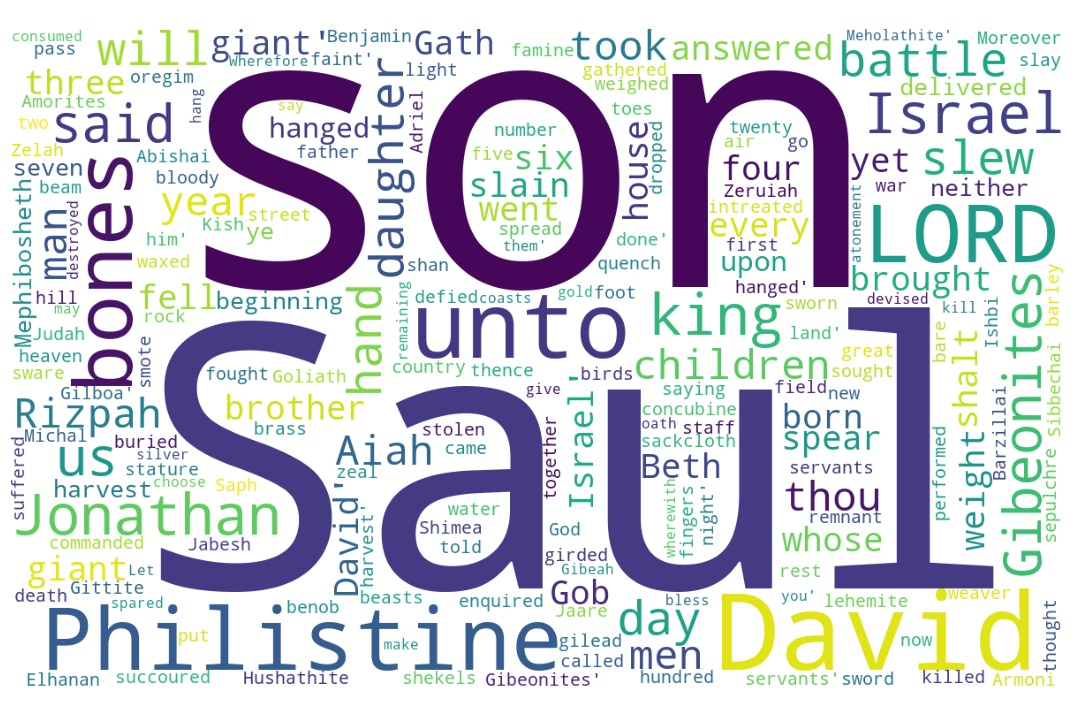
\includegraphics[width=\linewidth]{10OT-2Samuel/2Samuel21-WordCloud.jpg}
  \caption{1 Samuel 21 Word Cloud}
  \label{fig:1 Samuel 21 Word Cloud}
\end{figure}

%%%%%%%%%%%%%%%%%%%%%%%%%%%%%%%%%%%%%%%%%
%%%%%%%%%%%%%%%%%%%%%%%%%%%%%%%%%%%%%%%%%

\marginpar{\scriptsize \centering \fcolorbox{bone}{lime}{\textbf{GIANTS FINALLY DEFEATED}}\\ (2 Samuel 21:1--22) 
\begin{compactenum}[I.][8]
   \item   \textbf{Barren} Days \index[scripture]{2Samuel!2Sa 21:01} (2Sa 21:1) 
   \item The  \textbf{Betrayal} Disclosed \index[scripture]{2Samuel!2Sa 21:01} (2Sa 21:1) 
   \item A  \textbf{Bloody} Death \index[scripture]{2Samuel!2Sa 21:09} (2Sa 21:9) 
   \item The  \textbf{Brothers} Delivered \index[scripture]{2Samuel!2Sa 21:09} (2Sa 21:9) 
   \item   \textbf{Burial} Described \index[scripture]{2Samuel!2Sa 21:14} (2Sa 21:14) 
   \item   \textbf{Bones} Deposited \index[scripture]{2Samuel!2Sa 21:14} (2Sa 21:14) 
   \item Goliath's  \textbf{Brothers} Defeated \index[scripture]{2Samuel!2Sa 21:22} (2Sa 21:22) 
\end{compactenum} }

\footnote{\textcolor[cmyk]{0.99998,1,0,0}{\hyperlink{TOC}{Return to end of Table of Contents.}}}\footnote{\href{https://audiobible.com/bible/2_samuel_21.html}{\textcolor[cmyk]{0.99998,1,0,0}{2 Samuel 21 Audio}}}\textcolor[cmyk]{0.99998,1,0,0}{Then there was a \fcolorbox{bone}{lime}{famine} in the days of David three years, year after year; and David enquired of the LORD. And the LORD answered, \emph{It} \emph{is} for \fcolorbox{bone}{bone}{Saul}, and for \emph{his} \fcolorbox{bone}{lime}{bloody house}, because he slew the Gibeonites.}
[2] \textcolor[cmyk]{0.99998,1,0,0}{And the king called the Gibeonites, and said unto them; (now the Gibeonites \emph{were} not of the children of Israel, but of the remnant of the Amorites; and the children of Israel had sworn unto them: and \fcolorbox{bone}{bone}{Saul} sought to slay them in his zeal to the children of Israel and Judah.)}
[3] \textcolor[cmyk]{0.99998,1,0,0}{Wherefore David said unto the Gibeonites, What shall I do for you? and wherewith shall I make the atonement, that ye may bless the inheritance of the LORD?}
[4] \textcolor[cmyk]{0.99998,1,0,0}{And the Gibeonites said unto him, We will have no silver nor gold of \fcolorbox{bone}{bone}{Saul}, nor of his house; neither for us shalt thou kill any man in Israel. And he said, What ye shall say, \emph{that} will I do for you.}
[5] \textcolor[cmyk]{0.99998,1,0,0}{And they answered the king, The man that consumed us, and that devised against us \emph{that} we should be destroyed from remaining in any of the coasts of Israel,}
[6] \textcolor[cmyk]{0.99998,1,0,0}{Let seven men of his sons be delivered unto us, and we will hang them up unto the LORD in Gibeah of \fcolorbox{bone}{bone}{Saul}, \emph{whom} the LORD did choose. And the king said, I will give \emph{them}.}
[7] \textcolor[cmyk]{0.99998,1,0,0}{But the king spared Mephibosheth, the son of Jonathan the son of \fcolorbox{bone}{bone}{Saul}, because of the LORD'S oath that \emph{was} between them, between David and Jonathan the son of \fcolorbox{bone}{bone}{Saul}.}
[8] \textcolor[cmyk]{0.99998,1,0,0}{But the king took the two sons of Rizpah the daughter of Aiah, whom she bare unto \fcolorbox{bone}{bone}{Saul}, Armoni and Mephibosheth; and the five sons of Michal the daughter of \fcolorbox{bone}{bone}{Saul}, whom she brought up for Adriel the son of Barzillai the Meholathite:}
[9] \textcolor[cmyk]{0.99998,1,0,0}{And he \fcolorbox{bone}{lime}{delivered} them into the hands of the Gibeonites, and they hanged them in the hill before the LORD: and they fell \emph{all} seven together, and were \fcolorbox{bone}{lime}{put to death} in the days of harvest, in the first \emph{days}, in the beginning of barley harvest.}\\
\\
\P \textcolor[cmyk]{0.99998,1,0,0}{And Rizpah the daughter of Aiah took sackcloth, and spread it for her upon the rock, from the beginning of harvest until water dropped upon them out of heaven, and suffered neither the birds of the air to rest on them by day, nor the beasts of the field by night.}
[11] \textcolor[cmyk]{0.99998,1,0,0}{And it was told David what Rizpah the daughter of Aiah, the concubine of \fcolorbox{bone}{bone}{Saul}, had done.}\\
\\
\P \textcolor[cmyk]{0.99998,1,0,0}{And David went and took the bones of \fcolorbox{bone}{bone}{Saul} and the bones of Jonathan his son from the men of \fcolorbox{bone}{MYGOLD}{Jabesh-gilead}, which had stolen them from the street of Beth-shan, where the Philistines had hanged them, when the Philistines had slain \fcolorbox{bone}{bone}{Saul} in Gilboa:}
[13] \textcolor[cmyk]{0.99998,1,0,0}{And he brought up from thence the bones of \fcolorbox{bone}{bone}{Saul} and the bones of Jonathan his son; and they gathered the bones of them that were hanged.}
[14] \textcolor[cmyk]{0.99998,1,0,0}{And the \fcolorbox{bone}{lime}{bones} of \fcolorbox{bone}{bone}{Saul} and Jonathan his son \fcolorbox{bone}{lime}{buried} they in the country of Benjamin in Zelah, in the sepulchre of Kish his father: and they performed all that the king commanded. And after that God was intreated for the land.}\\
\\
\P \textcolor[cmyk]{0.99998,1,0,0}{Moreover the Philistines had yet war again with Israel; and David went down, and his servants with him, and fought against the Philistines: and David waxed faint.}
[16] \textcolor[cmyk]{0.99998,1,0,0}{And Ishbi-benob, which \emph{was} of the sons of the giant, the weight of whose spear \emph{weighed} three hundred \emph{shekels} of brass in weight, he being girded with a new \emph{sword}, thought to have slain David.}
[17] \textcolor[cmyk]{0.99998,1,0,0}{But Abishai the son of Zeruiah succoured him, and smote the Philistine, and killed him. Then the men of David sware unto him, saying, Thou shalt go no more out with us to battle, that thou quench not the light of Israel.}
[18] \textcolor[cmyk]{0.99998,1,0,0}{And it came to pass after this, that there was again a battle with the Philistines at Gob: then Sibbechai the Hushathite slew Saph, which \emph{was} of the sons of the giant.}
[19] \textcolor[cmyk]{0.99998,1,0,0}{And there was again a battle in Gob with the Philistines, where Elhanan the son of Jaare-oregim, a \fcolorbox{bone}{MYGOLD}{Beth-lehemite}, slew \emph{the} \emph{brother} \emph{of} Goliath the Gittite, the staff of whose spear \emph{was} like a weaver's beam.}
[20] \textcolor[cmyk]{0.99998,1,0,0}{And there was yet a battle in Gath, where was a man of \emph{great} stature, that had on every hand six fingers, and on every foot six toes, four and twenty in number; and he also was born to the giant.}
[21] \textcolor[cmyk]{0.99998,1,0,0}{And when he defied Israel, Jonathan the son of Shimea the brother of David slew him.}
[22] \textcolor[cmyk]{0.99998,1,0,0}{These four were born to the giant in Gath, and \fcolorbox{bone}{lime}{fell by the hand of David}, and by the hand of his servants.}
\index[NWIV]{39!2Samuel!2Sa 21:1}\index[AWIP]{Then!2Samuel!2Sa 21:1}\index[AWIP]{there!2Samuel!2Sa 21:1}\index[AWIP]{was!2Samuel!2Sa 21:1}\index[AWIP]{a!2Samuel!2Sa 21:1}\index[AWIP]{famine!2Samuel!2Sa 21:1}\index[AWIP]{in!2Samuel!2Sa 21:1}\index[AWIP]{the!2Samuel!2Sa 21:1}\index[AWIP]{the!2Samuel!2Sa 21:1 (2)}\index[AWIP]{the!2Samuel!2Sa 21:1 (3)}\index[AWIP]{the!2Samuel!2Sa 21:1 (4)}\index[AWIP]{days!2Samuel!2Sa 21:1}\index[AWIP]{of!2Samuel!2Sa 21:1}\index[AWIP]{of!2Samuel!2Sa 21:1 (2)}\index[AWIP]{David!2Samuel!2Sa 21:1}\index[AWIP]{David!2Samuel!2Sa 21:1 (2)}\index[AWIP]{three!2Samuel!2Sa 21:1}\index[AWIP]{years!2Samuel!2Sa 21:1}\index[AWIP]{year!2Samuel!2Sa 21:1}\index[AWIP]{year!2Samuel!2Sa 21:1 (2)}\index[AWIP]{after!2Samuel!2Sa 21:1}\index[AWIP]{and!2Samuel!2Sa 21:1}\index[AWIP]{and!2Samuel!2Sa 21:1 (2)}\index[AWIP]{enquired!2Samuel!2Sa 21:1}\index[AWIP]{LORD!2Samuel!2Sa 21:1}\index[AWIP]{LORD!2Samuel!2Sa 21:1 (2)}\index[AWIP]{And!2Samuel!2Sa 21:1}\index[AWIP]{answered!2Samuel!2Sa 21:1}\index[AWIP]{\emph{It}!2Samuel!2Sa 21:1}\index[AWIP]{\emph{is}!2Samuel!2Sa 21:1}\index[AWIP]{for!2Samuel!2Sa 21:1}\index[AWIP]{for!2Samuel!2Sa 21:1 (2)}\index[AWIP]{Saul!2Samuel!2Sa 21:1}\index[AWIP]{\emph{his}!2Samuel!2Sa 21:1}\index[AWIP]{bloody!2Samuel!2Sa 21:1}\index[AWIP]{house!2Samuel!2Sa 21:1}\index[AWIP]{because!2Samuel!2Sa 21:1}\index[AWIP]{he!2Samuel!2Sa 21:1}\index[AWIP]{slew!2Samuel!2Sa 21:1}\index[AWIP]{Gibeonites!2Samuel!2Sa 21:1}\index[AWIP]{\emph{It}!2Samuel!2Sa 21:1}\index[AWIP]{\emph{is}!2Samuel!2Sa 21:1}\index[AWIP]{\emph{his}!2Samuel!2Sa 21:1}

\index[NWIV]{52!2Samuel!2Sa 21:2}\index[AWIP]{And!2Samuel!2Sa 21:2}\index[AWIP]{the!2Samuel!2Sa 21:2}\index[AWIP]{the!2Samuel!2Sa 21:2 (2)}\index[AWIP]{the!2Samuel!2Sa 21:2 (3)}\index[AWIP]{the!2Samuel!2Sa 21:2 (4)}\index[AWIP]{the!2Samuel!2Sa 21:2 (5)}\index[AWIP]{the!2Samuel!2Sa 21:2 (6)}\index[AWIP]{the!2Samuel!2Sa 21:2 (7)}\index[AWIP]{the!2Samuel!2Sa 21:2 (8)}\index[AWIP]{king!2Samuel!2Sa 21:2}\index[AWIP]{called!2Samuel!2Sa 21:2}\index[AWIP]{Gibeonites!2Samuel!2Sa 21:2}\index[AWIP]{Gibeonites!2Samuel!2Sa 21:2 (2)}\index[AWIP]{and!2Samuel!2Sa 21:2}\index[AWIP]{and!2Samuel!2Sa 21:2 (2)}\index[AWIP]{and!2Samuel!2Sa 21:2 (3)}\index[AWIP]{and!2Samuel!2Sa 21:2 (4)}\index[AWIP]{said!2Samuel!2Sa 21:2}\index[AWIP]{unto!2Samuel!2Sa 21:2}\index[AWIP]{unto!2Samuel!2Sa 21:2 (2)}\index[AWIP]{them!2Samuel!2Sa 21:2}\index[AWIP]{them!2Samuel!2Sa 21:2 (2)}\index[AWIP]{them!2Samuel!2Sa 21:2 (3)}\index[AWIP]{(now!2Samuel!2Sa 21:2}\index[AWIP]{\emph{were}!2Samuel!2Sa 21:2}\index[AWIP]{not!2Samuel!2Sa 21:2}\index[AWIP]{of!2Samuel!2Sa 21:2}\index[AWIP]{of!2Samuel!2Sa 21:2 (2)}\index[AWIP]{of!2Samuel!2Sa 21:2 (3)}\index[AWIP]{of!2Samuel!2Sa 21:2 (4)}\index[AWIP]{of!2Samuel!2Sa 21:2 (5)}\index[AWIP]{of!2Samuel!2Sa 21:2 (6)}\index[AWIP]{children!2Samuel!2Sa 21:2}\index[AWIP]{children!2Samuel!2Sa 21:2 (2)}\index[AWIP]{children!2Samuel!2Sa 21:2 (3)}\index[AWIP]{Israel!2Samuel!2Sa 21:2}\index[AWIP]{Israel!2Samuel!2Sa 21:2 (2)}\index[AWIP]{Israel!2Samuel!2Sa 21:2 (3)}\index[AWIP]{but!2Samuel!2Sa 21:2}\index[AWIP]{remnant!2Samuel!2Sa 21:2}\index[AWIP]{Amorites!2Samuel!2Sa 21:2}\index[AWIP]{had!2Samuel!2Sa 21:2}\index[AWIP]{sworn!2Samuel!2Sa 21:2}\index[AWIP]{Saul!2Samuel!2Sa 21:2}\index[AWIP]{sought!2Samuel!2Sa 21:2}\index[AWIP]{to!2Samuel!2Sa 21:2}\index[AWIP]{to!2Samuel!2Sa 21:2 (2)}\index[AWIP]{slay!2Samuel!2Sa 21:2}\index[AWIP]{in!2Samuel!2Sa 21:2}\index[AWIP]{his!2Samuel!2Sa 21:2}\index[AWIP]{zeal!2Samuel!2Sa 21:2}\index[AWIP]{Judah)!2Samuel!2Sa 21:2}\index[AWIP]{\emph{were}!2Samuel!2Sa 21:2}

\index[NWIV]{28!2Samuel!2Sa 21:3}\index[AWIP]{Wherefore!2Samuel!2Sa 21:3}\index[AWIP]{David!2Samuel!2Sa 21:3}\index[AWIP]{said!2Samuel!2Sa 21:3}\index[AWIP]{unto!2Samuel!2Sa 21:3}\index[AWIP]{the!2Samuel!2Sa 21:3}\index[AWIP]{the!2Samuel!2Sa 21:3 (2)}\index[AWIP]{the!2Samuel!2Sa 21:3 (3)}\index[AWIP]{the!2Samuel!2Sa 21:3 (4)}\index[AWIP]{Gibeonites!2Samuel!2Sa 21:3}\index[AWIP]{What!2Samuel!2Sa 21:3}\index[AWIP]{shall!2Samuel!2Sa 21:3}\index[AWIP]{shall!2Samuel!2Sa 21:3 (2)}\index[AWIP]{I!2Samuel!2Sa 21:3}\index[AWIP]{I!2Samuel!2Sa 21:3 (2)}\index[AWIP]{do!2Samuel!2Sa 21:3}\index[AWIP]{for!2Samuel!2Sa 21:3}\index[AWIP]{you?!2Samuel!2Sa 21:3}\index[AWIP]{and!2Samuel!2Sa 21:3}\index[AWIP]{wherewith!2Samuel!2Sa 21:3}\index[AWIP]{make!2Samuel!2Sa 21:3}\index[AWIP]{atonement!2Samuel!2Sa 21:3}\index[AWIP]{that!2Samuel!2Sa 21:3}\index[AWIP]{ye!2Samuel!2Sa 21:3}\index[AWIP]{may!2Samuel!2Sa 21:3}\index[AWIP]{bless!2Samuel!2Sa 21:3}\index[AWIP]{inheritance!2Samuel!2Sa 21:3}\index[AWIP]{of!2Samuel!2Sa 21:3}\index[AWIP]{LORD?!2Samuel!2Sa 21:3}

\index[NWIV]{42!2Samuel!2Sa 21:4}\index[AWIP]{And!2Samuel!2Sa 21:4}\index[AWIP]{And!2Samuel!2Sa 21:4 (2)}\index[AWIP]{the!2Samuel!2Sa 21:4}\index[AWIP]{Gibeonites!2Samuel!2Sa 21:4}\index[AWIP]{said!2Samuel!2Sa 21:4}\index[AWIP]{said!2Samuel!2Sa 21:4 (2)}\index[AWIP]{unto!2Samuel!2Sa 21:4}\index[AWIP]{him!2Samuel!2Sa 21:4}\index[AWIP]{We!2Samuel!2Sa 21:4}\index[AWIP]{will!2Samuel!2Sa 21:4}\index[AWIP]{will!2Samuel!2Sa 21:4 (2)}\index[AWIP]{have!2Samuel!2Sa 21:4}\index[AWIP]{no!2Samuel!2Sa 21:4}\index[AWIP]{silver!2Samuel!2Sa 21:4}\index[AWIP]{nor!2Samuel!2Sa 21:4}\index[AWIP]{nor!2Samuel!2Sa 21:4 (2)}\index[AWIP]{gold!2Samuel!2Sa 21:4}\index[AWIP]{of!2Samuel!2Sa 21:4}\index[AWIP]{of!2Samuel!2Sa 21:4 (2)}\index[AWIP]{Saul!2Samuel!2Sa 21:4}\index[AWIP]{his!2Samuel!2Sa 21:4}\index[AWIP]{house!2Samuel!2Sa 21:4}\index[AWIP]{neither!2Samuel!2Sa 21:4}\index[AWIP]{for!2Samuel!2Sa 21:4}\index[AWIP]{for!2Samuel!2Sa 21:4 (2)}\index[AWIP]{us!2Samuel!2Sa 21:4}\index[AWIP]{shalt!2Samuel!2Sa 21:4}\index[AWIP]{thou!2Samuel!2Sa 21:4}\index[AWIP]{kill!2Samuel!2Sa 21:4}\index[AWIP]{any!2Samuel!2Sa 21:4}\index[AWIP]{man!2Samuel!2Sa 21:4}\index[AWIP]{in!2Samuel!2Sa 21:4}\index[AWIP]{Israel!2Samuel!2Sa 21:4}\index[AWIP]{he!2Samuel!2Sa 21:4}\index[AWIP]{What!2Samuel!2Sa 21:4}\index[AWIP]{ye!2Samuel!2Sa 21:4}\index[AWIP]{shall!2Samuel!2Sa 21:4}\index[AWIP]{say!2Samuel!2Sa 21:4}\index[AWIP]{\emph{that}!2Samuel!2Sa 21:4}\index[AWIP]{I!2Samuel!2Sa 21:4}\index[AWIP]{do!2Samuel!2Sa 21:4}\index[AWIP]{you!2Samuel!2Sa 21:4}\index[AWIP]{\emph{that}!2Samuel!2Sa 21:4}

\index[NWIV]{29!2Samuel!2Sa 21:5}\index[AWIP]{And!2Samuel!2Sa 21:5}\index[AWIP]{they!2Samuel!2Sa 21:5}\index[AWIP]{answered!2Samuel!2Sa 21:5}\index[AWIP]{the!2Samuel!2Sa 21:5}\index[AWIP]{the!2Samuel!2Sa 21:5 (2)}\index[AWIP]{king!2Samuel!2Sa 21:5}\index[AWIP]{The!2Samuel!2Sa 21:5}\index[AWIP]{man!2Samuel!2Sa 21:5}\index[AWIP]{that!2Samuel!2Sa 21:5}\index[AWIP]{that!2Samuel!2Sa 21:5 (2)}\index[AWIP]{consumed!2Samuel!2Sa 21:5}\index[AWIP]{us!2Samuel!2Sa 21:5}\index[AWIP]{us!2Samuel!2Sa 21:5 (2)}\index[AWIP]{and!2Samuel!2Sa 21:5}\index[AWIP]{devised!2Samuel!2Sa 21:5}\index[AWIP]{against!2Samuel!2Sa 21:5}\index[AWIP]{\emph{that}!2Samuel!2Sa 21:5}\index[AWIP]{we!2Samuel!2Sa 21:5}\index[AWIP]{should!2Samuel!2Sa 21:5}\index[AWIP]{be!2Samuel!2Sa 21:5}\index[AWIP]{destroyed!2Samuel!2Sa 21:5}\index[AWIP]{from!2Samuel!2Sa 21:5}\index[AWIP]{remaining!2Samuel!2Sa 21:5}\index[AWIP]{in!2Samuel!2Sa 21:5}\index[AWIP]{any!2Samuel!2Sa 21:5}\index[AWIP]{of!2Samuel!2Sa 21:5}\index[AWIP]{of!2Samuel!2Sa 21:5 (2)}\index[AWIP]{coasts!2Samuel!2Sa 21:5}\index[AWIP]{Israel!2Samuel!2Sa 21:5}\index[AWIP]{\emph{that}!2Samuel!2Sa 21:5}

\index[NWIV]{36!2Samuel!2Sa 21:6}\index[AWIP]{Let!2Samuel!2Sa 21:6}\index[AWIP]{seven!2Samuel!2Sa 21:6}\index[AWIP]{men!2Samuel!2Sa 21:6}\index[AWIP]{of!2Samuel!2Sa 21:6}\index[AWIP]{of!2Samuel!2Sa 21:6 (2)}\index[AWIP]{his!2Samuel!2Sa 21:6}\index[AWIP]{sons!2Samuel!2Sa 21:6}\index[AWIP]{be!2Samuel!2Sa 21:6}\index[AWIP]{delivered!2Samuel!2Sa 21:6}\index[AWIP]{unto!2Samuel!2Sa 21:6}\index[AWIP]{unto!2Samuel!2Sa 21:6 (2)}\index[AWIP]{us!2Samuel!2Sa 21:6}\index[AWIP]{and!2Samuel!2Sa 21:6}\index[AWIP]{we!2Samuel!2Sa 21:6}\index[AWIP]{will!2Samuel!2Sa 21:6}\index[AWIP]{will!2Samuel!2Sa 21:6 (2)}\index[AWIP]{hang!2Samuel!2Sa 21:6}\index[AWIP]{them!2Samuel!2Sa 21:6}\index[AWIP]{up!2Samuel!2Sa 21:6}\index[AWIP]{the!2Samuel!2Sa 21:6}\index[AWIP]{the!2Samuel!2Sa 21:6 (2)}\index[AWIP]{the!2Samuel!2Sa 21:6 (3)}\index[AWIP]{LORD!2Samuel!2Sa 21:6}\index[AWIP]{LORD!2Samuel!2Sa 21:6 (2)}\index[AWIP]{in!2Samuel!2Sa 21:6}\index[AWIP]{Gibeah!2Samuel!2Sa 21:6}\index[AWIP]{Saul!2Samuel!2Sa 21:6}\index[AWIP]{\emph{whom}!2Samuel!2Sa 21:6}\index[AWIP]{did!2Samuel!2Sa 21:6}\index[AWIP]{choose!2Samuel!2Sa 21:6}\index[AWIP]{And!2Samuel!2Sa 21:6}\index[AWIP]{king!2Samuel!2Sa 21:6}\index[AWIP]{said!2Samuel!2Sa 21:6}\index[AWIP]{I!2Samuel!2Sa 21:6}\index[AWIP]{give!2Samuel!2Sa 21:6}\index[AWIP]{\emph{them}!2Samuel!2Sa 21:6}\index[AWIP]{\emph{whom}!2Samuel!2Sa 21:6}\index[AWIP]{\emph{them}!2Samuel!2Sa 21:6}

\index[NWIV]{30!2Samuel!2Sa 21:7}\index[AWIP]{But!2Samuel!2Sa 21:7}\index[AWIP]{the!2Samuel!2Sa 21:7}\index[AWIP]{the!2Samuel!2Sa 21:7 (2)}\index[AWIP]{the!2Samuel!2Sa 21:7 (3)}\index[AWIP]{the!2Samuel!2Sa 21:7 (4)}\index[AWIP]{the!2Samuel!2Sa 21:7 (5)}\index[AWIP]{king!2Samuel!2Sa 21:7}\index[AWIP]{spared!2Samuel!2Sa 21:7}\index[AWIP]{Mephibosheth!2Samuel!2Sa 21:7}\index[AWIP]{son!2Samuel!2Sa 21:7}\index[AWIP]{son!2Samuel!2Sa 21:7 (2)}\index[AWIP]{son!2Samuel!2Sa 21:7 (3)}\index[AWIP]{of!2Samuel!2Sa 21:7}\index[AWIP]{of!2Samuel!2Sa 21:7 (2)}\index[AWIP]{of!2Samuel!2Sa 21:7 (3)}\index[AWIP]{of!2Samuel!2Sa 21:7 (4)}\index[AWIP]{Jonathan!2Samuel!2Sa 21:7}\index[AWIP]{Jonathan!2Samuel!2Sa 21:7 (2)}\index[AWIP]{Saul!2Samuel!2Sa 21:7}\index[AWIP]{Saul!2Samuel!2Sa 21:7 (2)}\index[AWIP]{because!2Samuel!2Sa 21:7}\index[AWIP]{LORD'S!2Samuel!2Sa 21:7}\index[AWIP]{oath!2Samuel!2Sa 21:7}\index[AWIP]{that!2Samuel!2Sa 21:7}\index[AWIP]{\emph{was}!2Samuel!2Sa 21:7}\index[AWIP]{between!2Samuel!2Sa 21:7}\index[AWIP]{between!2Samuel!2Sa 21:7 (2)}\index[AWIP]{them!2Samuel!2Sa 21:7}\index[AWIP]{David!2Samuel!2Sa 21:7}\index[AWIP]{and!2Samuel!2Sa 21:7}\index[AWIP]{\emph{was}!2Samuel!2Sa 21:7}

\index[NWIV]{43!2Samuel!2Sa 21:8}\index[AWIP]{But!2Samuel!2Sa 21:8}\index[AWIP]{the!2Samuel!2Sa 21:8}\index[AWIP]{the!2Samuel!2Sa 21:8 (2)}\index[AWIP]{the!2Samuel!2Sa 21:8 (3)}\index[AWIP]{the!2Samuel!2Sa 21:8 (4)}\index[AWIP]{the!2Samuel!2Sa 21:8 (5)}\index[AWIP]{the!2Samuel!2Sa 21:8 (6)}\index[AWIP]{the!2Samuel!2Sa 21:8 (7)}\index[AWIP]{king!2Samuel!2Sa 21:8}\index[AWIP]{took!2Samuel!2Sa 21:8}\index[AWIP]{two!2Samuel!2Sa 21:8}\index[AWIP]{sons!2Samuel!2Sa 21:8}\index[AWIP]{sons!2Samuel!2Sa 21:8 (2)}\index[AWIP]{of!2Samuel!2Sa 21:8}\index[AWIP]{of!2Samuel!2Sa 21:8 (2)}\index[AWIP]{of!2Samuel!2Sa 21:8 (3)}\index[AWIP]{of!2Samuel!2Sa 21:8 (4)}\index[AWIP]{of!2Samuel!2Sa 21:8 (5)}\index[AWIP]{Rizpah!2Samuel!2Sa 21:8}\index[AWIP]{daughter!2Samuel!2Sa 21:8}\index[AWIP]{daughter!2Samuel!2Sa 21:8 (2)}\index[AWIP]{Aiah!2Samuel!2Sa 21:8}\index[AWIP]{whom!2Samuel!2Sa 21:8}\index[AWIP]{whom!2Samuel!2Sa 21:8 (2)}\index[AWIP]{she!2Samuel!2Sa 21:8}\index[AWIP]{she!2Samuel!2Sa 21:8 (2)}\index[AWIP]{bare!2Samuel!2Sa 21:8}\index[AWIP]{unto!2Samuel!2Sa 21:8}\index[AWIP]{Saul!2Samuel!2Sa 21:8}\index[AWIP]{Saul!2Samuel!2Sa 21:8 (2)}\index[AWIP]{Armoni!2Samuel!2Sa 21:8}\index[AWIP]{and!2Samuel!2Sa 21:8}\index[AWIP]{and!2Samuel!2Sa 21:8 (2)}\index[AWIP]{Mephibosheth!2Samuel!2Sa 21:8}\index[AWIP]{five!2Samuel!2Sa 21:8}\index[AWIP]{Michal!2Samuel!2Sa 21:8}\index[AWIP]{brought!2Samuel!2Sa 21:8}\index[AWIP]{up!2Samuel!2Sa 21:8}\index[AWIP]{for!2Samuel!2Sa 21:8}\index[AWIP]{Adriel!2Samuel!2Sa 21:8}\index[AWIP]{son!2Samuel!2Sa 21:8}\index[AWIP]{Barzillai!2Samuel!2Sa 21:8}\index[AWIP]{Meholathite!2Samuel!2Sa 21:8}

\index[NWIV]{46!2Samuel!2Sa 21:9}\index[AWIP]{And!2Samuel!2Sa 21:9}\index[AWIP]{he!2Samuel!2Sa 21:9}\index[AWIP]{delivered!2Samuel!2Sa 21:9}\index[AWIP]{them!2Samuel!2Sa 21:9}\index[AWIP]{them!2Samuel!2Sa 21:9 (2)}\index[AWIP]{into!2Samuel!2Sa 21:9}\index[AWIP]{the!2Samuel!2Sa 21:9}\index[AWIP]{the!2Samuel!2Sa 21:9 (2)}\index[AWIP]{the!2Samuel!2Sa 21:9 (3)}\index[AWIP]{the!2Samuel!2Sa 21:9 (4)}\index[AWIP]{the!2Samuel!2Sa 21:9 (5)}\index[AWIP]{the!2Samuel!2Sa 21:9 (6)}\index[AWIP]{the!2Samuel!2Sa 21:9 (7)}\index[AWIP]{hands!2Samuel!2Sa 21:9}\index[AWIP]{of!2Samuel!2Sa 21:9}\index[AWIP]{of!2Samuel!2Sa 21:9 (2)}\index[AWIP]{of!2Samuel!2Sa 21:9 (3)}\index[AWIP]{Gibeonites!2Samuel!2Sa 21:9}\index[AWIP]{and!2Samuel!2Sa 21:9}\index[AWIP]{and!2Samuel!2Sa 21:9 (2)}\index[AWIP]{and!2Samuel!2Sa 21:9 (3)}\index[AWIP]{they!2Samuel!2Sa 21:9}\index[AWIP]{they!2Samuel!2Sa 21:9 (2)}\index[AWIP]{hanged!2Samuel!2Sa 21:9}\index[AWIP]{in!2Samuel!2Sa 21:9}\index[AWIP]{in!2Samuel!2Sa 21:9 (2)}\index[AWIP]{in!2Samuel!2Sa 21:9 (3)}\index[AWIP]{in!2Samuel!2Sa 21:9 (4)}\index[AWIP]{hill!2Samuel!2Sa 21:9}\index[AWIP]{before!2Samuel!2Sa 21:9}\index[AWIP]{LORD!2Samuel!2Sa 21:9}\index[AWIP]{fell!2Samuel!2Sa 21:9}\index[AWIP]{\emph{all}!2Samuel!2Sa 21:9}\index[AWIP]{seven!2Samuel!2Sa 21:9}\index[AWIP]{together!2Samuel!2Sa 21:9}\index[AWIP]{were!2Samuel!2Sa 21:9}\index[AWIP]{put!2Samuel!2Sa 21:9}\index[AWIP]{to!2Samuel!2Sa 21:9}\index[AWIP]{death!2Samuel!2Sa 21:9}\index[AWIP]{days!2Samuel!2Sa 21:9}\index[AWIP]{harvest!2Samuel!2Sa 21:9}\index[AWIP]{harvest!2Samuel!2Sa 21:9 (2)}\index[AWIP]{first!2Samuel!2Sa 21:9}\index[AWIP]{\emph{days}!2Samuel!2Sa 21:9}\index[AWIP]{beginning!2Samuel!2Sa 21:9}\index[AWIP]{barley!2Samuel!2Sa 21:9}\index[AWIP]{\emph{all}!2Samuel!2Sa 21:9}\index[AWIP]{\emph{days}!2Samuel!2Sa 21:9}

\index[NWIV]{51!2Samuel!2Sa 21:10}\index[AWIP]{And!2Samuel!2Sa 21:10}\index[AWIP]{Rizpah!2Samuel!2Sa 21:10}\index[AWIP]{the!2Samuel!2Sa 21:10}\index[AWIP]{the!2Samuel!2Sa 21:10 (2)}\index[AWIP]{the!2Samuel!2Sa 21:10 (3)}\index[AWIP]{the!2Samuel!2Sa 21:10 (4)}\index[AWIP]{the!2Samuel!2Sa 21:10 (5)}\index[AWIP]{the!2Samuel!2Sa 21:10 (6)}\index[AWIP]{the!2Samuel!2Sa 21:10 (7)}\index[AWIP]{daughter!2Samuel!2Sa 21:10}\index[AWIP]{of!2Samuel!2Sa 21:10}\index[AWIP]{of!2Samuel!2Sa 21:10 (2)}\index[AWIP]{of!2Samuel!2Sa 21:10 (3)}\index[AWIP]{of!2Samuel!2Sa 21:10 (4)}\index[AWIP]{of!2Samuel!2Sa 21:10 (5)}\index[AWIP]{Aiah!2Samuel!2Sa 21:10}\index[AWIP]{took!2Samuel!2Sa 21:10}\index[AWIP]{sackcloth!2Samuel!2Sa 21:10}\index[AWIP]{and!2Samuel!2Sa 21:10}\index[AWIP]{and!2Samuel!2Sa 21:10 (2)}\index[AWIP]{spread!2Samuel!2Sa 21:10}\index[AWIP]{it!2Samuel!2Sa 21:10}\index[AWIP]{for!2Samuel!2Sa 21:10}\index[AWIP]{her!2Samuel!2Sa 21:10}\index[AWIP]{upon!2Samuel!2Sa 21:10}\index[AWIP]{upon!2Samuel!2Sa 21:10 (2)}\index[AWIP]{rock!2Samuel!2Sa 21:10}\index[AWIP]{from!2Samuel!2Sa 21:10}\index[AWIP]{beginning!2Samuel!2Sa 21:10}\index[AWIP]{harvest!2Samuel!2Sa 21:10}\index[AWIP]{until!2Samuel!2Sa 21:10}\index[AWIP]{water!2Samuel!2Sa 21:10}\index[AWIP]{dropped!2Samuel!2Sa 21:10}\index[AWIP]{them!2Samuel!2Sa 21:10}\index[AWIP]{them!2Samuel!2Sa 21:10 (2)}\index[AWIP]{out!2Samuel!2Sa 21:10}\index[AWIP]{heaven!2Samuel!2Sa 21:10}\index[AWIP]{suffered!2Samuel!2Sa 21:10}\index[AWIP]{neither!2Samuel!2Sa 21:10}\index[AWIP]{birds!2Samuel!2Sa 21:10}\index[AWIP]{air!2Samuel!2Sa 21:10}\index[AWIP]{to!2Samuel!2Sa 21:10}\index[AWIP]{rest!2Samuel!2Sa 21:10}\index[AWIP]{on!2Samuel!2Sa 21:10}\index[AWIP]{by!2Samuel!2Sa 21:10}\index[AWIP]{by!2Samuel!2Sa 21:10 (2)}\index[AWIP]{day!2Samuel!2Sa 21:10}\index[AWIP]{nor!2Samuel!2Sa 21:10}\index[AWIP]{beasts!2Samuel!2Sa 21:10}\index[AWIP]{field!2Samuel!2Sa 21:10}\index[AWIP]{night!2Samuel!2Sa 21:10}

\index[NWIV]{17!2Samuel!2Sa 21:11}\index[AWIP]{And!2Samuel!2Sa 21:11}\index[AWIP]{it!2Samuel!2Sa 21:11}\index[AWIP]{was!2Samuel!2Sa 21:11}\index[AWIP]{told!2Samuel!2Sa 21:11}\index[AWIP]{David!2Samuel!2Sa 21:11}\index[AWIP]{what!2Samuel!2Sa 21:11}\index[AWIP]{Rizpah!2Samuel!2Sa 21:11}\index[AWIP]{the!2Samuel!2Sa 21:11}\index[AWIP]{the!2Samuel!2Sa 21:11 (2)}\index[AWIP]{daughter!2Samuel!2Sa 21:11}\index[AWIP]{of!2Samuel!2Sa 21:11}\index[AWIP]{of!2Samuel!2Sa 21:11 (2)}\index[AWIP]{Aiah!2Samuel!2Sa 21:11}\index[AWIP]{concubine!2Samuel!2Sa 21:11}\index[AWIP]{Saul!2Samuel!2Sa 21:11}\index[AWIP]{had!2Samuel!2Sa 21:11}\index[AWIP]{done!2Samuel!2Sa 21:11}

\index[NWIV]{44!2Samuel!2Sa 21:12}\index[AWIP]{And!2Samuel!2Sa 21:12}\index[AWIP]{David!2Samuel!2Sa 21:12}\index[AWIP]{went!2Samuel!2Sa 21:12}\index[AWIP]{and!2Samuel!2Sa 21:12}\index[AWIP]{and!2Samuel!2Sa 21:12 (2)}\index[AWIP]{took!2Samuel!2Sa 21:12}\index[AWIP]{the!2Samuel!2Sa 21:12}\index[AWIP]{the!2Samuel!2Sa 21:12 (2)}\index[AWIP]{the!2Samuel!2Sa 21:12 (3)}\index[AWIP]{the!2Samuel!2Sa 21:12 (4)}\index[AWIP]{the!2Samuel!2Sa 21:12 (5)}\index[AWIP]{the!2Samuel!2Sa 21:12 (6)}\index[AWIP]{bones!2Samuel!2Sa 21:12}\index[AWIP]{bones!2Samuel!2Sa 21:12 (2)}\index[AWIP]{of!2Samuel!2Sa 21:12}\index[AWIP]{of!2Samuel!2Sa 21:12 (2)}\index[AWIP]{of!2Samuel!2Sa 21:12 (3)}\index[AWIP]{of!2Samuel!2Sa 21:12 (4)}\index[AWIP]{Saul!2Samuel!2Sa 21:12}\index[AWIP]{Saul!2Samuel!2Sa 21:12 (2)}\index[AWIP]{Jonathan!2Samuel!2Sa 21:12}\index[AWIP]{his!2Samuel!2Sa 21:12}\index[AWIP]{son!2Samuel!2Sa 21:12}\index[AWIP]{from!2Samuel!2Sa 21:12}\index[AWIP]{from!2Samuel!2Sa 21:12 (2)}\index[AWIP]{men!2Samuel!2Sa 21:12}\index[AWIP]{Jabesh-gilead!2Samuel!2Sa 21:12}\index[AWIP]{which!2Samuel!2Sa 21:12}\index[AWIP]{had!2Samuel!2Sa 21:12}\index[AWIP]{had!2Samuel!2Sa 21:12 (2)}\index[AWIP]{had!2Samuel!2Sa 21:12 (3)}\index[AWIP]{stolen!2Samuel!2Sa 21:12}\index[AWIP]{them!2Samuel!2Sa 21:12}\index[AWIP]{them!2Samuel!2Sa 21:12 (2)}\index[AWIP]{street!2Samuel!2Sa 21:12}\index[AWIP]{Beth-shan!2Samuel!2Sa 21:12}\index[AWIP]{where!2Samuel!2Sa 21:12}\index[AWIP]{Philistines!2Samuel!2Sa 21:12}\index[AWIP]{Philistines!2Samuel!2Sa 21:12 (2)}\index[AWIP]{hanged!2Samuel!2Sa 21:12}\index[AWIP]{when!2Samuel!2Sa 21:12}\index[AWIP]{slain!2Samuel!2Sa 21:12}\index[AWIP]{in!2Samuel!2Sa 21:12}\index[AWIP]{Gilboa!2Samuel!2Sa 21:12}

\index[NWIV]{27!2Samuel!2Sa 21:13}\index[AWIP]{And!2Samuel!2Sa 21:13}\index[AWIP]{he!2Samuel!2Sa 21:13}\index[AWIP]{brought!2Samuel!2Sa 21:13}\index[AWIP]{up!2Samuel!2Sa 21:13}\index[AWIP]{from!2Samuel!2Sa 21:13}\index[AWIP]{thence!2Samuel!2Sa 21:13}\index[AWIP]{the!2Samuel!2Sa 21:13}\index[AWIP]{the!2Samuel!2Sa 21:13 (2)}\index[AWIP]{the!2Samuel!2Sa 21:13 (3)}\index[AWIP]{bones!2Samuel!2Sa 21:13}\index[AWIP]{bones!2Samuel!2Sa 21:13 (2)}\index[AWIP]{bones!2Samuel!2Sa 21:13 (3)}\index[AWIP]{of!2Samuel!2Sa 21:13}\index[AWIP]{of!2Samuel!2Sa 21:13 (2)}\index[AWIP]{of!2Samuel!2Sa 21:13 (3)}\index[AWIP]{Saul!2Samuel!2Sa 21:13}\index[AWIP]{and!2Samuel!2Sa 21:13}\index[AWIP]{and!2Samuel!2Sa 21:13 (2)}\index[AWIP]{Jonathan!2Samuel!2Sa 21:13}\index[AWIP]{his!2Samuel!2Sa 21:13}\index[AWIP]{son!2Samuel!2Sa 21:13}\index[AWIP]{they!2Samuel!2Sa 21:13}\index[AWIP]{gathered!2Samuel!2Sa 21:13}\index[AWIP]{them!2Samuel!2Sa 21:13}\index[AWIP]{that!2Samuel!2Sa 21:13}\index[AWIP]{were!2Samuel!2Sa 21:13}\index[AWIP]{hanged!2Samuel!2Sa 21:13}

\index[NWIV]{42!2Samuel!2Sa 21:14}\index[AWIP]{And!2Samuel!2Sa 21:14}\index[AWIP]{And!2Samuel!2Sa 21:14 (2)}\index[AWIP]{the!2Samuel!2Sa 21:14}\index[AWIP]{the!2Samuel!2Sa 21:14 (2)}\index[AWIP]{the!2Samuel!2Sa 21:14 (3)}\index[AWIP]{the!2Samuel!2Sa 21:14 (4)}\index[AWIP]{the!2Samuel!2Sa 21:14 (5)}\index[AWIP]{bones!2Samuel!2Sa 21:14}\index[AWIP]{of!2Samuel!2Sa 21:14}\index[AWIP]{of!2Samuel!2Sa 21:14 (2)}\index[AWIP]{of!2Samuel!2Sa 21:14 (3)}\index[AWIP]{Saul!2Samuel!2Sa 21:14}\index[AWIP]{and!2Samuel!2Sa 21:14}\index[AWIP]{and!2Samuel!2Sa 21:14 (2)}\index[AWIP]{Jonathan!2Samuel!2Sa 21:14}\index[AWIP]{his!2Samuel!2Sa 21:14}\index[AWIP]{his!2Samuel!2Sa 21:14 (2)}\index[AWIP]{son!2Samuel!2Sa 21:14}\index[AWIP]{buried!2Samuel!2Sa 21:14}\index[AWIP]{they!2Samuel!2Sa 21:14}\index[AWIP]{they!2Samuel!2Sa 21:14 (2)}\index[AWIP]{in!2Samuel!2Sa 21:14}\index[AWIP]{in!2Samuel!2Sa 21:14 (2)}\index[AWIP]{in!2Samuel!2Sa 21:14 (3)}\index[AWIP]{country!2Samuel!2Sa 21:14}\index[AWIP]{Benjamin!2Samuel!2Sa 21:14}\index[AWIP]{Zelah!2Samuel!2Sa 21:14}\index[AWIP]{sepulchre!2Samuel!2Sa 21:14}\index[AWIP]{Kish!2Samuel!2Sa 21:14}\index[AWIP]{father!2Samuel!2Sa 21:14}\index[AWIP]{performed!2Samuel!2Sa 21:14}\index[AWIP]{all!2Samuel!2Sa 21:14}\index[AWIP]{that!2Samuel!2Sa 21:14}\index[AWIP]{that!2Samuel!2Sa 21:14 (2)}\index[AWIP]{king!2Samuel!2Sa 21:14}\index[AWIP]{commanded!2Samuel!2Sa 21:14}\index[AWIP]{after!2Samuel!2Sa 21:14}\index[AWIP]{God!2Samuel!2Sa 21:14}\index[AWIP]{was!2Samuel!2Sa 21:14}\index[AWIP]{intreated!2Samuel!2Sa 21:14}\index[AWIP]{for!2Samuel!2Sa 21:14}\index[AWIP]{land!2Samuel!2Sa 21:14}

\index[NWIV]{27!2Samuel!2Sa 21:15}\index[AWIP]{Moreover!2Samuel!2Sa 21:15}\index[AWIP]{the!2Samuel!2Sa 21:15}\index[AWIP]{the!2Samuel!2Sa 21:15 (2)}\index[AWIP]{Philistines!2Samuel!2Sa 21:15}\index[AWIP]{Philistines!2Samuel!2Sa 21:15 (2)}\index[AWIP]{had!2Samuel!2Sa 21:15}\index[AWIP]{yet!2Samuel!2Sa 21:15}\index[AWIP]{war!2Samuel!2Sa 21:15}\index[AWIP]{again!2Samuel!2Sa 21:15}\index[AWIP]{with!2Samuel!2Sa 21:15}\index[AWIP]{with!2Samuel!2Sa 21:15 (2)}\index[AWIP]{Israel!2Samuel!2Sa 21:15}\index[AWIP]{and!2Samuel!2Sa 21:15}\index[AWIP]{and!2Samuel!2Sa 21:15 (2)}\index[AWIP]{and!2Samuel!2Sa 21:15 (3)}\index[AWIP]{and!2Samuel!2Sa 21:15 (4)}\index[AWIP]{David!2Samuel!2Sa 21:15}\index[AWIP]{David!2Samuel!2Sa 21:15 (2)}\index[AWIP]{went!2Samuel!2Sa 21:15}\index[AWIP]{down!2Samuel!2Sa 21:15}\index[AWIP]{his!2Samuel!2Sa 21:15}\index[AWIP]{servants!2Samuel!2Sa 21:15}\index[AWIP]{him!2Samuel!2Sa 21:15}\index[AWIP]{fought!2Samuel!2Sa 21:15}\index[AWIP]{against!2Samuel!2Sa 21:15}\index[AWIP]{waxed!2Samuel!2Sa 21:15}\index[AWIP]{faint!2Samuel!2Sa 21:15}

\index[NWIV]{35!2Samuel!2Sa 21:16}\index[AWIP]{And!2Samuel!2Sa 21:16}\index[AWIP]{Ishbi-benob!2Samuel!2Sa 21:16}\index[AWIP]{which!2Samuel!2Sa 21:16}\index[AWIP]{\emph{was}!2Samuel!2Sa 21:16}\index[AWIP]{of!2Samuel!2Sa 21:16}\index[AWIP]{of!2Samuel!2Sa 21:16 (2)}\index[AWIP]{of!2Samuel!2Sa 21:16 (3)}\index[AWIP]{of!2Samuel!2Sa 21:16 (4)}\index[AWIP]{the!2Samuel!2Sa 21:16}\index[AWIP]{the!2Samuel!2Sa 21:16 (2)}\index[AWIP]{the!2Samuel!2Sa 21:16 (3)}\index[AWIP]{sons!2Samuel!2Sa 21:16}\index[AWIP]{giant!2Samuel!2Sa 21:16}\index[AWIP]{weight!2Samuel!2Sa 21:16}\index[AWIP]{weight!2Samuel!2Sa 21:16 (2)}\index[AWIP]{whose!2Samuel!2Sa 21:16}\index[AWIP]{spear!2Samuel!2Sa 21:16}\index[AWIP]{\emph{weighed}!2Samuel!2Sa 21:16}\index[AWIP]{three!2Samuel!2Sa 21:16}\index[AWIP]{hundred!2Samuel!2Sa 21:16}\index[AWIP]{\emph{shekels}!2Samuel!2Sa 21:16}\index[AWIP]{brass!2Samuel!2Sa 21:16}\index[AWIP]{in!2Samuel!2Sa 21:16}\index[AWIP]{he!2Samuel!2Sa 21:16}\index[AWIP]{being!2Samuel!2Sa 21:16}\index[AWIP]{girded!2Samuel!2Sa 21:16}\index[AWIP]{with!2Samuel!2Sa 21:16}\index[AWIP]{a!2Samuel!2Sa 21:16}\index[AWIP]{new!2Samuel!2Sa 21:16}\index[AWIP]{\emph{sword}!2Samuel!2Sa 21:16}\index[AWIP]{thought!2Samuel!2Sa 21:16}\index[AWIP]{to!2Samuel!2Sa 21:16}\index[AWIP]{have!2Samuel!2Sa 21:16}\index[AWIP]{slain!2Samuel!2Sa 21:16}\index[AWIP]{David!2Samuel!2Sa 21:16}\index[AWIP]{\emph{was}!2Samuel!2Sa 21:16}\index[AWIP]{\emph{weighed}!2Samuel!2Sa 21:16}\index[AWIP]{\emph{shekels}!2Samuel!2Sa 21:16}\index[AWIP]{\emph{sword}!2Samuel!2Sa 21:16}

\index[NWIV]{42!2Samuel!2Sa 21:17}\index[AWIP]{But!2Samuel!2Sa 21:17}\index[AWIP]{Abishai!2Samuel!2Sa 21:17}\index[AWIP]{the!2Samuel!2Sa 21:17}\index[AWIP]{the!2Samuel!2Sa 21:17 (2)}\index[AWIP]{the!2Samuel!2Sa 21:17 (3)}\index[AWIP]{the!2Samuel!2Sa 21:17 (4)}\index[AWIP]{son!2Samuel!2Sa 21:17}\index[AWIP]{of!2Samuel!2Sa 21:17}\index[AWIP]{of!2Samuel!2Sa 21:17 (2)}\index[AWIP]{of!2Samuel!2Sa 21:17 (3)}\index[AWIP]{Zeruiah!2Samuel!2Sa 21:17}\index[AWIP]{succoured!2Samuel!2Sa 21:17}\index[AWIP]{him!2Samuel!2Sa 21:17}\index[AWIP]{him!2Samuel!2Sa 21:17 (2)}\index[AWIP]{him!2Samuel!2Sa 21:17 (3)}\index[AWIP]{and!2Samuel!2Sa 21:17}\index[AWIP]{and!2Samuel!2Sa 21:17 (2)}\index[AWIP]{smote!2Samuel!2Sa 21:17}\index[AWIP]{Philistine!2Samuel!2Sa 21:17}\index[AWIP]{killed!2Samuel!2Sa 21:17}\index[AWIP]{Then!2Samuel!2Sa 21:17}\index[AWIP]{men!2Samuel!2Sa 21:17}\index[AWIP]{David!2Samuel!2Sa 21:17}\index[AWIP]{sware!2Samuel!2Sa 21:17}\index[AWIP]{unto!2Samuel!2Sa 21:17}\index[AWIP]{saying!2Samuel!2Sa 21:17}\index[AWIP]{Thou!2Samuel!2Sa 21:17}\index[AWIP]{shalt!2Samuel!2Sa 21:17}\index[AWIP]{go!2Samuel!2Sa 21:17}\index[AWIP]{no!2Samuel!2Sa 21:17}\index[AWIP]{more!2Samuel!2Sa 21:17}\index[AWIP]{out!2Samuel!2Sa 21:17}\index[AWIP]{with!2Samuel!2Sa 21:17}\index[AWIP]{us!2Samuel!2Sa 21:17}\index[AWIP]{to!2Samuel!2Sa 21:17}\index[AWIP]{battle!2Samuel!2Sa 21:17}\index[AWIP]{that!2Samuel!2Sa 21:17}\index[AWIP]{thou!2Samuel!2Sa 21:17}\index[AWIP]{quench!2Samuel!2Sa 21:17}\index[AWIP]{not!2Samuel!2Sa 21:17}\index[AWIP]{light!2Samuel!2Sa 21:17}\index[AWIP]{Israel!2Samuel!2Sa 21:17}

\index[NWIV]{32!2Samuel!2Sa 21:18}\index[AWIP]{And!2Samuel!2Sa 21:18}\index[AWIP]{it!2Samuel!2Sa 21:18}\index[AWIP]{came!2Samuel!2Sa 21:18}\index[AWIP]{to!2Samuel!2Sa 21:18}\index[AWIP]{pass!2Samuel!2Sa 21:18}\index[AWIP]{after!2Samuel!2Sa 21:18}\index[AWIP]{this!2Samuel!2Sa 21:18}\index[AWIP]{that!2Samuel!2Sa 21:18}\index[AWIP]{there!2Samuel!2Sa 21:18}\index[AWIP]{was!2Samuel!2Sa 21:18}\index[AWIP]{again!2Samuel!2Sa 21:18}\index[AWIP]{a!2Samuel!2Sa 21:18}\index[AWIP]{battle!2Samuel!2Sa 21:18}\index[AWIP]{with!2Samuel!2Sa 21:18}\index[AWIP]{the!2Samuel!2Sa 21:18}\index[AWIP]{the!2Samuel!2Sa 21:18 (2)}\index[AWIP]{the!2Samuel!2Sa 21:18 (3)}\index[AWIP]{the!2Samuel!2Sa 21:18 (4)}\index[AWIP]{Philistines!2Samuel!2Sa 21:18}\index[AWIP]{at!2Samuel!2Sa 21:18}\index[AWIP]{Gob!2Samuel!2Sa 21:18}\index[AWIP]{then!2Samuel!2Sa 21:18}\index[AWIP]{Sibbechai!2Samuel!2Sa 21:18}\index[AWIP]{Hushathite!2Samuel!2Sa 21:18}\index[AWIP]{slew!2Samuel!2Sa 21:18}\index[AWIP]{Saph!2Samuel!2Sa 21:18}\index[AWIP]{which!2Samuel!2Sa 21:18}\index[AWIP]{\emph{was}!2Samuel!2Sa 21:18}\index[AWIP]{of!2Samuel!2Sa 21:18}\index[AWIP]{of!2Samuel!2Sa 21:18 (2)}\index[AWIP]{sons!2Samuel!2Sa 21:18}\index[AWIP]{giant!2Samuel!2Sa 21:18}\index[AWIP]{\emph{was}!2Samuel!2Sa 21:18}

\index[NWIV]{36!2Samuel!2Sa 21:19}\index[AWIP]{And!2Samuel!2Sa 21:19}\index[AWIP]{there!2Samuel!2Sa 21:19}\index[AWIP]{was!2Samuel!2Sa 21:19}\index[AWIP]{again!2Samuel!2Sa 21:19}\index[AWIP]{a!2Samuel!2Sa 21:19}\index[AWIP]{a!2Samuel!2Sa 21:19 (2)}\index[AWIP]{a!2Samuel!2Sa 21:19 (3)}\index[AWIP]{battle!2Samuel!2Sa 21:19}\index[AWIP]{in!2Samuel!2Sa 21:19}\index[AWIP]{Gob!2Samuel!2Sa 21:19}\index[AWIP]{with!2Samuel!2Sa 21:19}\index[AWIP]{the!2Samuel!2Sa 21:19}\index[AWIP]{the!2Samuel!2Sa 21:19 (2)}\index[AWIP]{the!2Samuel!2Sa 21:19 (3)}\index[AWIP]{the!2Samuel!2Sa 21:19 (4)}\index[AWIP]{Philistines!2Samuel!2Sa 21:19}\index[AWIP]{where!2Samuel!2Sa 21:19}\index[AWIP]{Elhanan!2Samuel!2Sa 21:19}\index[AWIP]{son!2Samuel!2Sa 21:19}\index[AWIP]{of!2Samuel!2Sa 21:19}\index[AWIP]{of!2Samuel!2Sa 21:19 (2)}\index[AWIP]{Jaare-oregim!2Samuel!2Sa 21:19}\index[AWIP]{Beth-lehemite!2Samuel!2Sa 21:19}\index[AWIP]{slew!2Samuel!2Sa 21:19}\index[AWIP]{\emph{the}!2Samuel!2Sa 21:19}\index[AWIP]{\emph{brother}!2Samuel!2Sa 21:19}\index[AWIP]{\emph{of}!2Samuel!2Sa 21:19}\index[AWIP]{Goliath!2Samuel!2Sa 21:19}\index[AWIP]{Gittite!2Samuel!2Sa 21:19}\index[AWIP]{staff!2Samuel!2Sa 21:19}\index[AWIP]{whose!2Samuel!2Sa 21:19}\index[AWIP]{spear!2Samuel!2Sa 21:19}\index[AWIP]{\emph{was}!2Samuel!2Sa 21:19}\index[AWIP]{like!2Samuel!2Sa 21:19}\index[AWIP]{weaver's!2Samuel!2Sa 21:19}\index[AWIP]{beam!2Samuel!2Sa 21:19}\index[AWIP]{\emph{the}!2Samuel!2Sa 21:19}\index[AWIP]{\emph{brother}!2Samuel!2Sa 21:19}\index[AWIP]{\emph{of}!2Samuel!2Sa 21:19}\index[AWIP]{\emph{was}!2Samuel!2Sa 21:19}

\index[NWIV]{41!2Samuel!2Sa 21:20}\index[AWIP]{And!2Samuel!2Sa 21:20}\index[AWIP]{there!2Samuel!2Sa 21:20}\index[AWIP]{was!2Samuel!2Sa 21:20}\index[AWIP]{was!2Samuel!2Sa 21:20 (2)}\index[AWIP]{was!2Samuel!2Sa 21:20 (3)}\index[AWIP]{yet!2Samuel!2Sa 21:20}\index[AWIP]{a!2Samuel!2Sa 21:20}\index[AWIP]{a!2Samuel!2Sa 21:20 (2)}\index[AWIP]{battle!2Samuel!2Sa 21:20}\index[AWIP]{in!2Samuel!2Sa 21:20}\index[AWIP]{in!2Samuel!2Sa 21:20 (2)}\index[AWIP]{Gath!2Samuel!2Sa 21:20}\index[AWIP]{where!2Samuel!2Sa 21:20}\index[AWIP]{man!2Samuel!2Sa 21:20}\index[AWIP]{of!2Samuel!2Sa 21:20}\index[AWIP]{\emph{great}!2Samuel!2Sa 21:20}\index[AWIP]{stature!2Samuel!2Sa 21:20}\index[AWIP]{that!2Samuel!2Sa 21:20}\index[AWIP]{had!2Samuel!2Sa 21:20}\index[AWIP]{on!2Samuel!2Sa 21:20}\index[AWIP]{on!2Samuel!2Sa 21:20 (2)}\index[AWIP]{every!2Samuel!2Sa 21:20}\index[AWIP]{every!2Samuel!2Sa 21:20 (2)}\index[AWIP]{hand!2Samuel!2Sa 21:20}\index[AWIP]{six!2Samuel!2Sa 21:20}\index[AWIP]{six!2Samuel!2Sa 21:20 (2)}\index[AWIP]{fingers!2Samuel!2Sa 21:20}\index[AWIP]{and!2Samuel!2Sa 21:20}\index[AWIP]{and!2Samuel!2Sa 21:20 (2)}\index[AWIP]{and!2Samuel!2Sa 21:20 (3)}\index[AWIP]{foot!2Samuel!2Sa 21:20}\index[AWIP]{toes!2Samuel!2Sa 21:20}\index[AWIP]{four!2Samuel!2Sa 21:20}\index[AWIP]{twenty!2Samuel!2Sa 21:20}\index[AWIP]{number!2Samuel!2Sa 21:20}\index[AWIP]{he!2Samuel!2Sa 21:20}\index[AWIP]{also!2Samuel!2Sa 21:20}\index[AWIP]{born!2Samuel!2Sa 21:20}\index[AWIP]{to!2Samuel!2Sa 21:20}\index[AWIP]{the!2Samuel!2Sa 21:20}\index[AWIP]{giant!2Samuel!2Sa 21:20}\index[AWIP]{\emph{great}!2Samuel!2Sa 21:20}

\index[NWIV]{16!2Samuel!2Sa 21:21}\index[AWIP]{And!2Samuel!2Sa 21:21}\index[AWIP]{when!2Samuel!2Sa 21:21}\index[AWIP]{he!2Samuel!2Sa 21:21}\index[AWIP]{defied!2Samuel!2Sa 21:21}\index[AWIP]{Israel!2Samuel!2Sa 21:21}\index[AWIP]{Jonathan!2Samuel!2Sa 21:21}\index[AWIP]{the!2Samuel!2Sa 21:21}\index[AWIP]{the!2Samuel!2Sa 21:21 (2)}\index[AWIP]{son!2Samuel!2Sa 21:21}\index[AWIP]{of!2Samuel!2Sa 21:21}\index[AWIP]{of!2Samuel!2Sa 21:21 (2)}\index[AWIP]{Shimea!2Samuel!2Sa 21:21}\index[AWIP]{brother!2Samuel!2Sa 21:21}\index[AWIP]{David!2Samuel!2Sa 21:21}\index[AWIP]{slew!2Samuel!2Sa 21:21}\index[AWIP]{him!2Samuel!2Sa 21:21}

\index[NWIV]{23!2Samuel!2Sa 21:22}\index[AWIP]{These!2Samuel!2Sa 21:22}\index[AWIP]{four!2Samuel!2Sa 21:22}\index[AWIP]{were!2Samuel!2Sa 21:22}\index[AWIP]{born!2Samuel!2Sa 21:22}\index[AWIP]{to!2Samuel!2Sa 21:22}\index[AWIP]{the!2Samuel!2Sa 21:22}\index[AWIP]{the!2Samuel!2Sa 21:22 (2)}\index[AWIP]{the!2Samuel!2Sa 21:22 (3)}\index[AWIP]{giant!2Samuel!2Sa 21:22}\index[AWIP]{in!2Samuel!2Sa 21:22}\index[AWIP]{Gath!2Samuel!2Sa 21:22}\index[AWIP]{and!2Samuel!2Sa 21:22}\index[AWIP]{and!2Samuel!2Sa 21:22 (2)}\index[AWIP]{fell!2Samuel!2Sa 21:22}\index[AWIP]{by!2Samuel!2Sa 21:22}\index[AWIP]{by!2Samuel!2Sa 21:22 (2)}\index[AWIP]{hand!2Samuel!2Sa 21:22}\index[AWIP]{hand!2Samuel!2Sa 21:22 (2)}\index[AWIP]{of!2Samuel!2Sa 21:22}\index[AWIP]{of!2Samuel!2Sa 21:22 (2)}\index[AWIP]{David!2Samuel!2Sa 21:22}\index[AWIP]{his!2Samuel!2Sa 21:22}\index[AWIP]{servants!2Samuel!2Sa 21:22}

\index[NWIV]{9!2Samuel!2Sa 21:23}\index[AWIP]{lso!2Samuel!2Sa 21:23}\index[AWIP]{the!2Samuel!2Sa 21:23}\index[AWIP]{Jairite!2Samuel!2Sa 21:23}\index[AWIP]{was!2Samuel!2Sa 21:23}\index[AWIP]{a!2Samuel!2Sa 21:23}\index[AWIP]{chief!2Samuel!2Sa 21:23}\index[AWIP]{ruler!2Samuel!2Sa 21:23}\index[AWIP]{about!2Samuel!2Sa 21:23}\index[AWIP]{David!2Samuel!2Sa 21:23}


\section{2 Samuel 21 Outlines}

\subsection{My Outlines}

\subsubsection{Giants Finally Defeated}

\index[speaker]{Keith Anthony!2 Samuel 21 (Giants Finally Defeated)}
\index[series]{2 Samuel (Keith Anthony)!2 Samuel 21 (Giants Finally Defeated)}
\index[date]{2018/04/10!12 Samuel 21 (Giants Finally Defeated) (Keith Anthony)}
\begin{compactenum}[I.]
   \item   \textbf{Barren} Days \index[scripture]{2Samuel!2Sa 21:01} (2Sa 21:1) 
   \item The  \textbf{Betrayal} Disclosed \index[scripture]{2Samuel!2Sa 21:01} (2Sa 21:1) 
   \item A  \textbf{Bloody} Death \index[scripture]{2Samuel!2Sa 21:09} (2Sa 21:9) 
   \item The  \textbf{Brothers} Delivered \index[scripture]{2Samuel!2Sa 21:09} (2Sa 21:9) 
   \item   \textbf{Burial} Described \index[scripture]{2Samuel!2Sa 21:14} (2Sa 21:14) 
   \item   \textbf{Bones} Deposited \index[scripture]{2Samuel!2Sa 21:14} (2Sa 21:14) 
   \item Goliath's  \textbf{Brothers} Defeated \index[scripture]{2Samuel!2Sa 21:22} (2Sa 21:22) 
\end{compactenum}


%\subsection{Outlines from Others}


\section{2 Samuel 21 Comments}

\subsection{Numeric Nuggets}
\textbf{13: } The name ``Saul'' is found 13 times in the chapter. The 13-character names ``Jabesh-gilead'' and ``Beth-lehemite'' are found in the chapter.

\chapter{Psalm 99}
\begin{figure}
  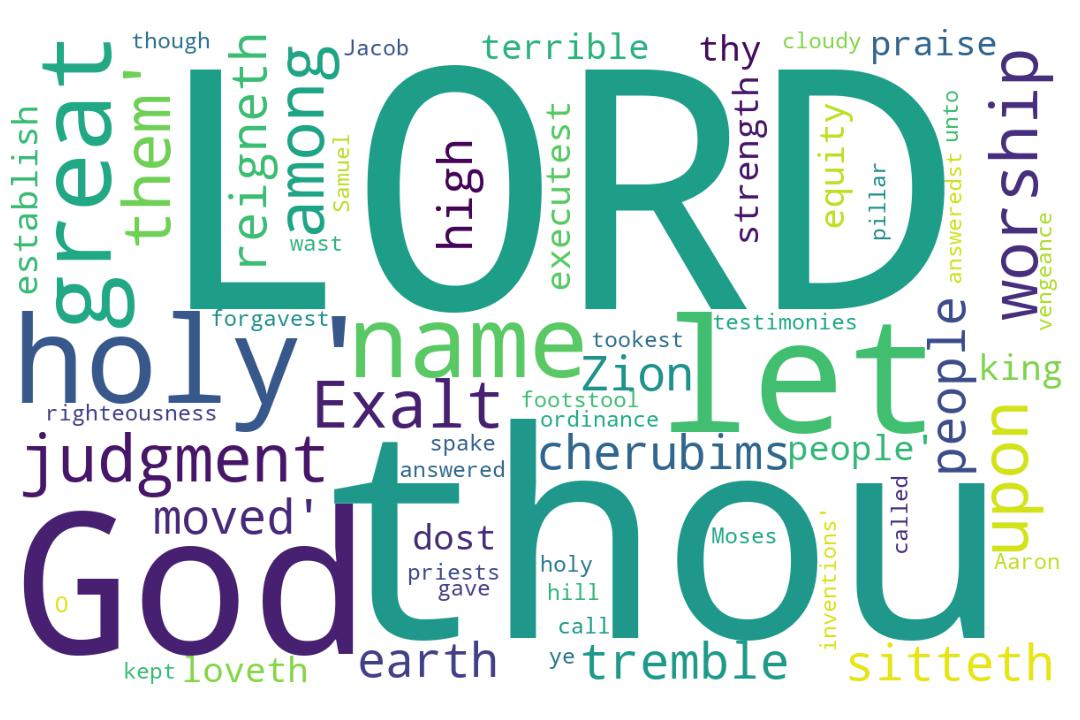
\includegraphics[width=\linewidth]{19OT-Psalms/Psalm99-WordCloud.jpg}
  \caption{Psalm 99 Word Cloud}
  \label{fig:Psalm 99 word Cloud}
\end{figure}

\marginpar{\scriptsize \centering \fcolorbox{bone}{lime}{\textbf{A PSALM OF KINGSHIP}}\\ (Psalm 99:1-9) \begin{compactenum}[I.][8]
    \item \textbf{Designation of God's Mastery} \index[scripture]{Psalms!Psa 099:01}(Psa 99:1)
    \item \textbf{Declaration of God's Might} \index[scripture]{Psalms!Psa 099:01-03}(Psa 99:1-3)
    \item \textbf{Description of God's Mercy} \index[scripture]{Psalms!Psa 099:04-05}(Psa 99:4-5)
    \item \textbf{Dealing with God's Moral Purity} \index[scripture]{Psalms!Psa 099:04}(Psa 99:4)
    \item \textbf{Dealings of God with the Multitude} \index[scripture]{Psalms!Psa 099:06-09}(Psa 99:6-9)
    \item A \textbf{Determination to Exalt God Methodically} \index[scripture]{Psalms!Psa 099:09}(Psa 99:9)
\end{compactenum}}

\footnote{\textcolor[cmyk]{0.99998,1,0,0}{\hyperlink{TOC}{Return to end of Table of Contents.}}}\footnote{\href{https://audiobible.com/bible/psalms_99.html}{\textcolor[cmyk]{0.99998,1,0,0}{Psalm 99 Audio}}}\textcolor[cmyk]{0.99998,1,0,0}{The LORD reigneth; let the people tremble: he sitteth \emph{between} the cherubims; \fcolorbox{bone}{lime}{let the earth be moved}.}
[2] \textcolor[cmyk]{0.99998,1,0,0}{The LORD \emph{is} great in Zion; and he \emph{is} high above all the people.}
[3] \textcolor[cmyk]{0.99998,1,0,0}{Let them praise thy great and terrible name; \emph{for} it \emph{is} holy.}
[4] \textcolor[cmyk]{0.99998,1,0,0}{The king's strength also loveth judgment; thou dost establish \fcolorbox{bone}{lime}{equity}, thou executest \fcolorbox{bone}{lime}{judgment and \fcolorbox{bone}{MYGOLD}{righteousness}} in Jacob.}
[5] \textcolor[cmyk]{0.99998,1,0,0}{Exalt ye the LORD our God, and worship at his footstool; \emph{for} he \emph{is} holy.}
[6] \textcolor[cmyk]{0.99998,1,0,0}{Moses and Aaron among his priests, and Samuel among them that call upon his name; they called upon the LORD, and he answered them.}
[7] \textcolor[cmyk]{0.99998,1,0,0}{He spake unto them in the cloudy pillar: they kept his testimonies, and the ordinance \emph{that} he gave them.}
[8] \textcolor[cmyk]{0.99998,1,0,0}{Thou \fcolorbox{bone}{lime}{answeredst} them, O LORD our God: thou wast a God that \fcolorbox{bone}{lime}{forgavest} them, though thou \fcolorbox{bone}{lime}{tookest vengeance} of their inventions.}
[9] \textcolor[cmyk]{0.99998,1,0,0}{\fcolorbox{bone}{lime}{Exalt} the LORD our God, and \fcolorbox{bone}{lime}{worship} at his holy hill; for the LORD our God \emph{is} holy.}
\index[NWIV]{17!Psalm!Psa 99:1}\index[AWIP]{The!Psalm!Psa 99:1}\index[AWIP]{LORD!Psalm!Psa 99:1}\index[AWIP]{reigneth!Psalm!Psa 99:1}\index[AWIP]{let!Psalm!Psa 99:1}\index[AWIP]{let!Psalm!Psa 99:1 (2)}\index[AWIP]{the!Psalm!Psa 99:1}\index[AWIP]{the!Psalm!Psa 99:1 (2)}\index[AWIP]{the!Psalm!Psa 99:1 (3)}\index[AWIP]{people!Psalm!Psa 99:1}\index[AWIP]{tremble!Psalm!Psa 99:1}\index[AWIP]{he!Psalm!Psa 99:1}\index[AWIP]{sitteth!Psalm!Psa 99:1}\index[AWIP]{\emph{between}!Psalm!Psa 99:1}\index[AWIP]{cherubims!Psalm!Psa 99:1}\index[AWIP]{earth!Psalm!Psa 99:1}\index[AWIP]{be!Psalm!Psa 99:1}\index[AWIP]{moved!Psalm!Psa 99:1}\index[AWIP]{\emph{between}!Psalm!Psa 99:1}

\index[NWIV]{14!Psalm!Psa 99:2}\index[AWIP]{The!Psalm!Psa 99:2}\index[AWIP]{LORD!Psalm!Psa 99:2}\index[AWIP]{\emph{is}!Psalm!Psa 99:2}\index[AWIP]{\emph{is}!Psalm!Psa 99:2 (2)}\index[AWIP]{great!Psalm!Psa 99:2}\index[AWIP]{in!Psalm!Psa 99:2}\index[AWIP]{Zion!Psalm!Psa 99:2}\index[AWIP]{and!Psalm!Psa 99:2}\index[AWIP]{he!Psalm!Psa 99:2}\index[AWIP]{high!Psalm!Psa 99:2}\index[AWIP]{above!Psalm!Psa 99:2}\index[AWIP]{all!Psalm!Psa 99:2}\index[AWIP]{the!Psalm!Psa 99:2}\index[AWIP]{people!Psalm!Psa 99:2}\index[AWIP]{\emph{is}!Psalm!Psa 99:2}\index[AWIP]{\emph{is}!Psalm!Psa 99:2 (2)}

\index[NWIV]{12!Psalm!Psa 99:3}\index[AWIP]{Let!Psalm!Psa 99:3}\index[AWIP]{them!Psalm!Psa 99:3}\index[AWIP]{praise!Psalm!Psa 99:3}\index[AWIP]{thy!Psalm!Psa 99:3}\index[AWIP]{great!Psalm!Psa 99:3}\index[AWIP]{and!Psalm!Psa 99:3}\index[AWIP]{terrible!Psalm!Psa 99:3}\index[AWIP]{name!Psalm!Psa 99:3}\index[AWIP]{\emph{for}!Psalm!Psa 99:3}\index[AWIP]{it!Psalm!Psa 99:3}\index[AWIP]{\emph{is}!Psalm!Psa 99:3}\index[AWIP]{holy!Psalm!Psa 99:3}\index[AWIP]{\emph{for}!Psalm!Psa 99:3}\index[AWIP]{\emph{is}!Psalm!Psa 99:3}

\index[NWIV]{17!Psalm!Psa 99:4}\index[AWIP]{The!Psalm!Psa 99:4}\index[AWIP]{king's!Psalm!Psa 99:4}\index[AWIP]{strength!Psalm!Psa 99:4}\index[AWIP]{also!Psalm!Psa 99:4}\index[AWIP]{loveth!Psalm!Psa 99:4}\index[AWIP]{judgment!Psalm!Psa 99:4}\index[AWIP]{judgment!Psalm!Psa 99:4 (2)}\index[AWIP]{thou!Psalm!Psa 99:4}\index[AWIP]{thou!Psalm!Psa 99:4 (2)}\index[AWIP]{dost!Psalm!Psa 99:4}\index[AWIP]{establish!Psalm!Psa 99:4}\index[AWIP]{equity!Psalm!Psa 99:4}\index[AWIP]{executest!Psalm!Psa 99:4}\index[AWIP]{and!Psalm!Psa 99:4}\index[AWIP]{righteousness!Psalm!Psa 99:4}\index[AWIP]{in!Psalm!Psa 99:4}\index[AWIP]{Jacob!Psalm!Psa 99:4}

\index[NWIV]{15!Psalm!Psa 99:5}\index[AWIP]{Exalt!Psalm!Psa 99:5}\index[AWIP]{ye!Psalm!Psa 99:5}\index[AWIP]{the!Psalm!Psa 99:5}\index[AWIP]{LORD!Psalm!Psa 99:5}\index[AWIP]{our!Psalm!Psa 99:5}\index[AWIP]{God!Psalm!Psa 99:5}\index[AWIP]{and!Psalm!Psa 99:5}\index[AWIP]{worship!Psalm!Psa 99:5}\index[AWIP]{at!Psalm!Psa 99:5}\index[AWIP]{his!Psalm!Psa 99:5}\index[AWIP]{footstool!Psalm!Psa 99:5}\index[AWIP]{\emph{for}!Psalm!Psa 99:5}\index[AWIP]{he!Psalm!Psa 99:5}\index[AWIP]{\emph{is}!Psalm!Psa 99:5}\index[AWIP]{holy!Psalm!Psa 99:5}\index[AWIP]{\emph{for}!Psalm!Psa 99:5}\index[AWIP]{\emph{is}!Psalm!Psa 99:5}

\index[NWIV]{24!Psalm!Psa 99:6}\index[AWIP]{Moses!Psalm!Psa 99:6}\index[AWIP]{and!Psalm!Psa 99:6}\index[AWIP]{and!Psalm!Psa 99:6 (2)}\index[AWIP]{and!Psalm!Psa 99:6 (3)}\index[AWIP]{Aaron!Psalm!Psa 99:6}\index[AWIP]{among!Psalm!Psa 99:6}\index[AWIP]{among!Psalm!Psa 99:6 (2)}\index[AWIP]{his!Psalm!Psa 99:6}\index[AWIP]{his!Psalm!Psa 99:6 (2)}\index[AWIP]{priests!Psalm!Psa 99:6}\index[AWIP]{Samuel!Psalm!Psa 99:6}\index[AWIP]{them!Psalm!Psa 99:6}\index[AWIP]{them!Psalm!Psa 99:6 (2)}\index[AWIP]{that!Psalm!Psa 99:6}\index[AWIP]{call!Psalm!Psa 99:6}\index[AWIP]{upon!Psalm!Psa 99:6}\index[AWIP]{upon!Psalm!Psa 99:6 (2)}\index[AWIP]{name!Psalm!Psa 99:6}\index[AWIP]{they!Psalm!Psa 99:6}\index[AWIP]{called!Psalm!Psa 99:6}\index[AWIP]{the!Psalm!Psa 99:6}\index[AWIP]{LORD!Psalm!Psa 99:6}\index[AWIP]{he!Psalm!Psa 99:6}\index[AWIP]{answered!Psalm!Psa 99:6}

\index[NWIV]{19!Psalm!Psa 99:7}\index[AWIP]{He!Psalm!Psa 99:7}\index[AWIP]{spake!Psalm!Psa 99:7}\index[AWIP]{unto!Psalm!Psa 99:7}\index[AWIP]{them!Psalm!Psa 99:7}\index[AWIP]{them!Psalm!Psa 99:7 (2)}\index[AWIP]{in!Psalm!Psa 99:7}\index[AWIP]{the!Psalm!Psa 99:7}\index[AWIP]{the!Psalm!Psa 99:7 (2)}\index[AWIP]{cloudy!Psalm!Psa 99:7}\index[AWIP]{pillar!Psalm!Psa 99:7}\index[AWIP]{they!Psalm!Psa 99:7}\index[AWIP]{kept!Psalm!Psa 99:7}\index[AWIP]{his!Psalm!Psa 99:7}\index[AWIP]{testimonies!Psalm!Psa 99:7}\index[AWIP]{and!Psalm!Psa 99:7}\index[AWIP]{ordinance!Psalm!Psa 99:7}\index[AWIP]{\emph{that}!Psalm!Psa 99:7}\index[AWIP]{he!Psalm!Psa 99:7}\index[AWIP]{gave!Psalm!Psa 99:7}\index[AWIP]{\emph{that}!Psalm!Psa 99:7}

\index[NWIV]{21!Psalm!Psa 99:8}\index[AWIP]{Thou!Psalm!Psa 99:8}\index[AWIP]{answeredst!Psalm!Psa 99:8}\index[AWIP]{them!Psalm!Psa 99:8}\index[AWIP]{them!Psalm!Psa 99:8 (2)}\index[AWIP]{O!Psalm!Psa 99:8}\index[AWIP]{LORD!Psalm!Psa 99:8}\index[AWIP]{our!Psalm!Psa 99:8}\index[AWIP]{God!Psalm!Psa 99:8}\index[AWIP]{God!Psalm!Psa 99:8 (2)}\index[AWIP]{thou!Psalm!Psa 99:8}\index[AWIP]{thou!Psalm!Psa 99:8 (2)}\index[AWIP]{wast!Psalm!Psa 99:8}\index[AWIP]{a!Psalm!Psa 99:8}\index[AWIP]{that!Psalm!Psa 99:8}\index[AWIP]{forgavest!Psalm!Psa 99:8}\index[AWIP]{though!Psalm!Psa 99:8}\index[AWIP]{tookest!Psalm!Psa 99:8}\index[AWIP]{vengeance!Psalm!Psa 99:8}\index[AWIP]{of!Psalm!Psa 99:8}\index[AWIP]{their!Psalm!Psa 99:8}\index[AWIP]{inventions!Psalm!Psa 99:8}

\index[NWIV]{18!Psalm!Psa 99:9}\index[AWIP]{Exalt!Psalm!Psa 99:9}\index[AWIP]{the!Psalm!Psa 99:9}\index[AWIP]{the!Psalm!Psa 99:9 (2)}\index[AWIP]{LORD!Psalm!Psa 99:9}\index[AWIP]{LORD!Psalm!Psa 99:9 (2)}\index[AWIP]{our!Psalm!Psa 99:9}\index[AWIP]{our!Psalm!Psa 99:9 (2)}\index[AWIP]{God!Psalm!Psa 99:9}\index[AWIP]{God!Psalm!Psa 99:9 (2)}\index[AWIP]{and!Psalm!Psa 99:9}\index[AWIP]{worship!Psalm!Psa 99:9}\index[AWIP]{at!Psalm!Psa 99:9}\index[AWIP]{his!Psalm!Psa 99:9}\index[AWIP]{holy!Psalm!Psa 99:9}\index[AWIP]{holy!Psalm!Psa 99:9 (2)}\index[AWIP]{hill!Psalm!Psa 99:9}\index[AWIP]{for!Psalm!Psa 99:9}\index[AWIP]{\emph{is}!Psalm!Psa 99:9}\index[AWIP]{\emph{is}!Psalm!Psa 99:9}


\section{Psalm 99 Outlines}

\subsection{My Outlines}

\subsubsection{A Psalm of Kingship}
\textbf{Introduction: }Psalm 99 (adapted from Ryrie):
\index[speaker]{Keith Anthony!Psalm 099 (A Psalm of Kingship)}
\index[series]{Psalms (Keith Anthony)!Psalm 099 (A Psalm of Kingship)}
\index[date]{2015/09/12!Psalm 099 (A Psalm of Kingship) (Keith Anthony)}

\begin{compactenum}[I.]
    \item \textbf{Designation God's Mastery} \index[scripture]{Psalms!Psa 099:01}(Psa 99:1)
    \item \textbf{Declaration of God's Might} \index[scripture]{Psalms!Psa 099:01-03}(Psa 99:1-3)
    \item \textbf{Description of God's Mercy} \index[scripture]{Psalms!Psa 099:04-05}(Psa 99:4-5)
    \item \textbf{Dealing with God's Moral Purity} \index[scripture]{Psalms!Psa 099:04}(Psa 99:4)
    \item \textbf{Dealings of God with the Multitude} \index[scripture]{Psalms!Psa 099:06-09}(Psa 99:6-9)
    \item A \textbf{Determination to Exalt God Methodically} \index[scripture]{Psalms!Psa 099:09}(Psa 99:9)
\end{compactenum}

\subsection{Outlines from Others}


\section{Psalm 99 Comments}

\subsection{Numeric Nuggets}
\textbf{13: } The 13-letter word ``righteousness'' is used in the chapter.

\subsection{Psalm 99 Introduction}
This is another Millennial psalm. Ruckman points out the erroneous placement of the psalm by trusted modern clergy!\cite{Ruckman1992PsalmsV2}
\begin{compactenum}[I.]
	\item Mt Zion is interpreted as the church because it is God's ``favorite place.''
	\item The entire earth should be in awe of God sitting in heaven a sthe universal ``Monarch.''
	\item Spurgeon says, the ``rule of God'' can be felt by Christians today.\cite{spurgeon2016treasury}
	\item The message of the psalm is the ``mediatorial reign'' of Jesus Christ and of church leaders.
\end{compactenum}
If one held to an Amillennial or Postmillennial system of theology then one could not read the psalm as it is written  or interpret it correctly. The Lord is NOT now sitting on an earthly throne, but he will. And, as seen in verse 2, it will be in Zion.

\subsection{Psalm 99:1}
Apparently there is a seat where God is sitting and this seat is between things called ``cherubims''. We find ``cherubims'' 38 times in the AV, and ``cherubim's'' once. The first mention of cherubims is found in Genesis 3:24 where they are guarding and preventing fallen Adam from getting to the tree of life in Eden.\footnote{\textbf{Genesis 3:24} - So he drove out the man; and he placed at the east of the garden of Eden Cherubims, and a flaming sword which turned every way, to keep the way of the tree of life.}

This seat between the cherubims is where God is now seated.\footnote{\textbf{Revelation 4:6-9} - And before the throne there was a sea of glass like unto crystal: and in the midst of the throne, and round about the throne, were four beasts full of eyes before and behind. [7] And the first beast was like a lion, and the second beast like a calf, and the third beast had a face as a man, and the fourth beast was like a flying eagle. [8] And the four beasts had each of them six wings about him; and they were full of eyes within: and they rest not day and night, saying, Holy, holy, holy, Lord God Almighty, which was, and is, and is to come. [9] And when those beasts give glory and honour and thanks to him that sat on the throne, who liveth for ever and ever,} This seat is connected to the mercy seat in Numbers 7:89.\footnote{\textbf{Numbers 7:89} - And when Moses was gone into the tabernacle of the congregation to speak with him, then he heard the voice of one speaking unto him from off the mercy seat that was upon the ark of testimony, from between the two cherubims: and he spake unto him.} ``Between the churubims'' is where God sat in the tablernacle in the wilderness (Exodus 25:22)\footnote{\textbf{Exodus 25:22} - And there I will meet with thee, and I will commune with thee from above the mercy seat, from between the two cherubims which are upon the ark of the testimony, of all things which I will give thee in commandment unto the children of Israel.} and where Jesus is pictured at his return (Ezekiel 1:20-28).\footnote{\textbf{Ezekiel 1:20-28} - Whithersoever the spirit was to go, they went, thither was their spirit to go; and the wheels were lifted up over against them: for the spirit of the living creature was in the wheels. [21] When those went, these went; and when those stood, these stood; and when those were lifted up from the earth, the wheels were lifted up over against them: for the spirit of the living creature was in the wheels. [22] And the likeness of the firmament upon the heads of the living creature was as the colour of the terrible crystal, stretched forth over their heads above. [23] And under the firmament were their wings straight, the one toward the other: every one had two, which covered on this side, and every one had two, which covered on that side, their bodies. [24] And when they went, I heard the noise of their wings, like the noise of great waters, as the voice of the Almighty, the voice of speech, as the noise of an host: when they stood, they let down their wings. [25] And there was a voice from the firmament that was over their heads, when they stood, and had let down their wings.
[26] And above the firmament that was over their heads was the likeness of a throne, as the appearance of a sapphire stone: and upon the likeness of the throne was the likeness as the appearance of a man above upon it. [27] And I saw as the colour of amber, as the appearance of fire round about within it, from the appearance of his loins even upward, and from the appearance of his loins even downward, I saw as it were the appearance of fire, and it had brightness round about. [28] As the appearance of the bow that is in the cloud in the day of rain, so was the appearance of the brightness round about. This was the appearance of the likeness of the glory of the LORD. And when I saw it, I fell upon my face, and I heard a voice of one that spake.}

One of these cherubim, the fifth, is none other than Satan, who in one of his imitations of God, also now has a seat (Revelation 2:13).\footnote{\textbf{Revelation 2:13} - I know thy works, and where thou dwellest, even where Satan’s seat is: and thou holdest fast my name, and hast not denied my faith, even in those days wherein Antipas was my faithful martyr, who was slain among you, where Satan dwelleth.} From this seat, a religious throne, Satan now does his business in the religions of the world (but isn't there really only one?).

\subsection{Psalm 99:2}
The Lord is not only ``figuratively'' high above the people, but he is literally above the people, as the Second Advent will flatten all the hills and mountains of the earth except for Jerusalem, aka Zion. Now, Zion is at the top of the universe, the sides of the north.\footnote{\textbf{Psalm 48:2} - Beautiful for situation, the joy of the whole earth, is mount Zion, on the sides of the north, the city of the great King.}\footnote{\textbf{Isaiah 14:13} - For thou hast said in thine heart, I will ascend into heaven, I will exalt my throne above the stars of God: I will sit also upon the mount of the congregation, in the sides of the north:}

\subsection{Psalm 99:5}
The ``footstool'' is the earth (See Psalm 110:1, Isaiah 66:1, and Matthew 5:35).\footnote{\textbf{Psalm 110:1} - The LORD said unto my Lord, Sit thou at my right hand, until I make thine enemies thy footstool}\footnote{\textbf{Isaiah 66:1} - Thus saith the LORD, The heaven is my throne, and the earth is my footstool: where is the house that ye build unto me? and where is the place of my rest}\footnote{\textbf{Matthew 5:35} - Nor by the earth; for it is his footstool: neither by Jerusalem; for it is the city of the great King.}

\subsection{Psalm 99:8}
The word ``invent'' is used once in the AV, in Amos 6:5, and is connected to ``them that are at ease in Zion.''\footnote{\textbf{Amos 6:5} - That chant to the sound of the viol, and invent to themselves instruments of musick, like David;} The word ``inventions is used 5 times, here and in  Psalm 106:29,\footnote{\textbf{Psalm 106:29} - Thus they provoked him to anger with their inventions: and the plague brake in upon them.} Psalm 106:39,\footnote{\textbf{Psalm 106:39} - Thus were they defiled with their own works, and went a whoring with their own inventions.} Proverb 8:12,\footnote{\textbf{Proverb 8:12} - I wisdom dwell with prudence, and find out knowledge of witty inventions. } and Ecclesiastes 7:29.\footnote{\textbf{Ecclesiastes 7:29} - Lo, this only have I found, that God hath made man upright; but they have sought out many inventions.} One thinks of the ``engines of war'' built by cunning men in the days of Uzziah (2 Chronicles 26:15).\footnote{\textbf{2 Chronicles 26:15} - And he made in Jerusalem engines, invented by cunning men, to be on the towers and upon the bulwarks, to shoot arrows and great stones withal. And his name spread far abroad; for he was marvellously helped, till he was strong.} These can be likened to the same used by Nebuchadnezzar against Tyre in Ezekiel 26:9.\footnote{\textbf{Ezekiel 26:9} - And he shall set engines of war against thy walls, and with his axes he shall break down thy towers.} The examples provided in scripture put an interesting perspective on the function of engineers among mankind. Typically, new technologies have vast potential to improve the temporary lot of mankind (although they do nothing to solve the sin problem), but almost without fail the end up contributing to laziness, licenteousness, and the abuse of power. The verse in Amos gives a counterexample of David inventing musical instruments, as we see referenced in various psalms.


\chapter{Proverb 9}

\begin{figure}
  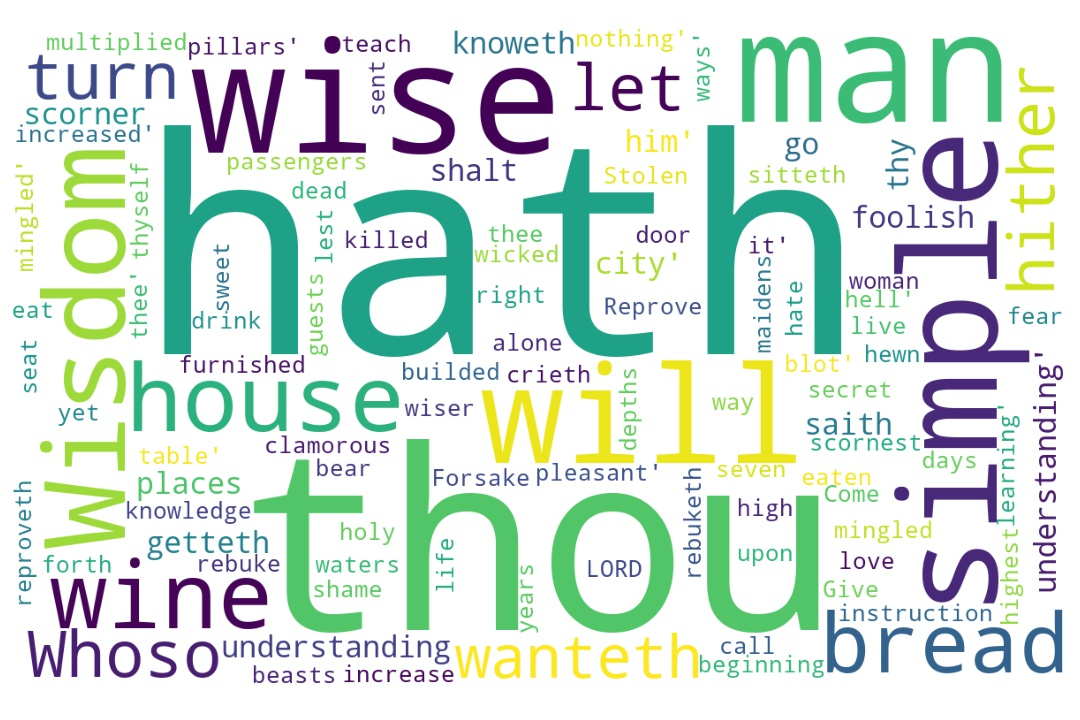
\includegraphics[width=\linewidth]{20OT-Proverbs/Proverb9-WordCloud.jpg}
  \caption{Proverb 9 Word Cloud}
  \label{fig:Proverb 9 Word Cloud}
\end{figure}


\marginpar{\scriptsize \centering \fcolorbox{bone}{lime}{\textbf{WISDOM: THE GOOD CHOICE}}\\ (Proverb 9:1-18) \begin{compactenum}[I.][8]
\item \textbf{Builds} a Life \index[scripture]{Proverbs!Pro 09:01}(Pro 9:1)
\item Has a \textbf{Banquet} \index[scripture]{Proverbs!Pro 09:02}(Pro 9:2)
\item Gives out \textbf{Bread} \index[scripture]{Proverbs!Pro 09:05}(Pro 9:5)
\item Has \textbf{Blessings} \index[scripture]{Proverbs!Pro 09:09}(Pro 9:9)
\item Was there from the \textbf{Beginning} \index[scripture]{Proverbs!Pro 09:10}(Pro 9:10)
\item Provides Lasting \textbf{Benefits} \index[scripture]{Proverbs!Pro 09:11}(Pro 9:11)
\item Is \textbf{Betrayed} \index[scripture]{Proverbs!Pro 09:13}(Pro 9:13)
\end{compactenum}}

\marginpar{\scriptsize \centering \fcolorbox{bone}{yellow}{\textbf{WISDOM AT WORK}}\\ (Proverb 9:1-18) \begin{compactenum}[I.][8]
    \item \textbf{Builds a House} \index[scripture]{Proverbs!Pro 09:01}(Pro 9:1)
    \item \textbf{Hews out Pillars} \index[scripture]{Proverbs!Pro 09:01}(Pro 9:1)
    \item \textbf{Kills her Beats} \index[scripture]{Proverbs!Pro 09:02}(Pro 9:2)
    \item \textbf{Mingles Her Wine} \index[scripture]{Proverbs!Pro 09:02}(Pro 9:2)
    \item \textbf{Furnishes her Table} \index[scripture]{Proverbs!Pro 09:02}(Pro 9:2)
    \item \textbf{Sends forthe her Maidens} \index[scripture]{Proverbs!Pro 09:03}(Pro 9:3)
    \item \textbf{Cries from the High Places} \index[scripture]{Proverbs!Pro 09:03}(Pro 9:3)
\end{compactenum}}

\marginpar{\scriptsize \centering \fcolorbox{bone}{black}{\textbf{\textcolor[cmyk]{0,0,0,0}{LOOKING FOR WISDOM}}}\\ (Proverb 9) 
\begin{compactenum}[I.][8]
    \item The \textbf{Rendering of Wisdom} \index[scripture]{Proverbs!Pro 09:01}(Pro 9:1) 
   \item The \textbf{Reaction to Wisdom} \index[scripture]{Proverbs!Pro 09:09}(Pro 9:9) 
    \item The \textbf{Reach for Wisdom} \index[scripture]{Proverbs!Pro 09:10}(Pro 9:10) 
    \item The \textbf{Road to Wisdom} \index[scripture]{Proverbs!Pro 09:11}(Pro 9:11) 
    \item The \textbf{Rejection of Wisdom} \index[scripture]{Proverbs!Pro 09:13}(Pro 9:13) 
    \item Man's \textbf{Regard \& Reverence for Foolishness} \index[scripture]{Proverbs!Pro 09:14}(Pro 9:14) 
    \item A \textbf{Reunion of Fools} \index[scripture]{Proverbs!Pro 09:15}(Pro 9:15) 
\end{compactenum}}

\footnote{\textcolor[cmyk]{0.99998,1,0,0}{\hyperlink{TOC}{Return to end of Table of Contents.}}}\footnote{\href{https://audiobible.com/bible/proverbs_9.html}{\textcolor[cmyk]{0.99998,1,0,0}{Proverbs Audio}}}\textcolor[cmyk]{0.99998,1,0,0}{Wisdom hath \fcolorbox{bone}{lime}{builded her house}, she hath hewn out her seven pillars:}\footnote{\textbf{1 Kings 8:27} - But will God indeed dwell on the earth? behold, the heaven and heaven of heavens cannot contain thee; how much less this house that I have builded?} 
[2] \textcolor[cmyk]{0.99998,1,0,0}{She hath killed her beasts; she hath mingled her wine; she hath also \fcolorbox{bone}{lime}{furnished} her table.}
[3] \textcolor[cmyk]{0.99998,1,0,0}{She hath sent forth her maidens: she crieth upon the highest places of the city,}
[4] \textcolor[cmyk]{0.99998,1,0,0}{Whoso \emph{is} simple, let him turn in hither: \emph{as} \emph{for} him that wanteth \fcolorbox{bone}{MYGOLD}{understanding}, she saith to him,}
[5] \textcolor[cmyk]{0.99998,1,0,0}{Come, \fcolorbox{bone}{lime}{eat of my} \fcolorbox{bone}{lime}{bread}, and drink of the wine \emph{which} I have mingled.}
[6] \textcolor[cmyk]{0.99998,1,0,0}{Forsake the foolish, and live; and go in the way of \fcolorbox{bone}{MYGOLD}{understanding}.}
[7] \textcolor[cmyk]{0.99998,1,0,0}{He that reproveth a scorner getteth to himself shame: and he that rebuketh a wicked \emph{man} \emph{getteth} himself a blot.}
[8] \textcolor[cmyk]{0.99998,1,0,0}{Reprove not a scorner, lest he hate thee: rebuke a wise man, and he will love thee.}
[9] \textcolor[cmyk]{0.99998,1,0,0}{Give \emph{instruction} to a wise \emph{man}, and he will \fcolorbox{bone}{lime}{be yet wiser}: teach a just \emph{man}, and he will increase in learning.}
[10] \textcolor[cmyk]{0.99998,1,0,0}{The fear of the LORD \emph{is} the \fcolorbox{bone}{lime}{beginning of wisdom}: and the knowledge of the holy \emph{is} \fcolorbox{bone}{MYGOLD}{understanding}.}
[11] \textcolor[cmyk]{0.99998,1,0,0}{For by me thy days shall be multiplied, and the years of thy life shall be \fcolorbox{bone}{lime}{increased}.}
[12] \textcolor[cmyk]{0.99998,1,0,0}{If thou be wise, thou shalt be wise for thyself: but \emph{if} thou scornest, thou alone shalt bear \emph{it}.}
[13] \textcolor[cmyk]{0.99998,1,0,0}{A foolish woman \emph{is} clamorous: \emph{she} \emph{is} simple, and \fcolorbox{bone}{lime}{knoweth nothing}.}
[14] \textcolor[cmyk]{0.99998,1,0,0}{For she sitteth at the door of her house, on a seat in the high places of the city,}
[15] \textcolor[cmyk]{0.99998,1,0,0}{To call passengers who go right on their ways:}
[16] \textcolor[cmyk]{0.99998,1,0,0}{Whoso \emph{is} simple, let him turn in hither: and \emph{as} \emph{for} him that wanteth \fcolorbox{bone}{MYGOLD}{understanding}, she saith to him,}
[17] \textcolor[cmyk]{0.99998,1,0,0}{Stolen waters are sweet, and bread \emph{eaten} in secret is pleasant.}
[18] \textcolor[cmyk]{0.99998,1,0,0}{But he knoweth not that the dead \emph{are} there; \emph{and} \emph{that} her guests \emph{are} in the depths of hell.}



\index[NWIV]{12!Proverbs!Pro 9:1}\index[AWIP]{Wisdom!Proverbs!Pro 9:1}\index[AWIP]{hath!Proverbs!Pro 9:1}\index[AWIP]{hath!Proverbs!Pro 9:1 (2)}\index[AWIP]{builded!Proverbs!Pro 9:1}\index[AWIP]{her!Proverbs!Pro 9:1}\index[AWIP]{her!Proverbs!Pro 9:1 (2)}\index[AWIP]{house!Proverbs!Pro 9:1}\index[AWIP]{she!Proverbs!Pro 9:1}\index[AWIP]{hewn!Proverbs!Pro 9:1}\index[AWIP]{out!Proverbs!Pro 9:1}\index[AWIP]{seven!Proverbs!Pro 9:1}\index[AWIP]{pillars!Proverbs!Pro 9:1}

\index[NWIV]{16!Proverbs!Pro 9:2}\index[AWIP]{She!Proverbs!Pro 9:2}\index[AWIP]{hath!Proverbs!Pro 9:2}\index[AWIP]{hath!Proverbs!Pro 9:2 (2)}\index[AWIP]{hath!Proverbs!Pro 9:2 (3)}\index[AWIP]{killed!Proverbs!Pro 9:2}\index[AWIP]{her!Proverbs!Pro 9:2}\index[AWIP]{her!Proverbs!Pro 9:2 (2)}\index[AWIP]{her!Proverbs!Pro 9:2 (3)}\index[AWIP]{beasts!Proverbs!Pro 9:2}\index[AWIP]{she!Proverbs!Pro 9:2}\index[AWIP]{she!Proverbs!Pro 9:2 (2)}\index[AWIP]{mingled!Proverbs!Pro 9:2}\index[AWIP]{wine!Proverbs!Pro 9:2}\index[AWIP]{also!Proverbs!Pro 9:2}\index[AWIP]{furnished!Proverbs!Pro 9:2}\index[AWIP]{table!Proverbs!Pro 9:2}

\index[NWIV]{15!Proverbs!Pro 9:3}\index[AWIP]{She!Proverbs!Pro 9:3}\index[AWIP]{hath!Proverbs!Pro 9:3}\index[AWIP]{sent!Proverbs!Pro 9:3}\index[AWIP]{forth!Proverbs!Pro 9:3}\index[AWIP]{her!Proverbs!Pro 9:3}\index[AWIP]{maidens!Proverbs!Pro 9:3}\index[AWIP]{she!Proverbs!Pro 9:3}\index[AWIP]{crieth!Proverbs!Pro 9:3}\index[AWIP]{upon!Proverbs!Pro 9:3}\index[AWIP]{the!Proverbs!Pro 9:3}\index[AWIP]{the!Proverbs!Pro 9:3 (2)}\index[AWIP]{highest!Proverbs!Pro 9:3}\index[AWIP]{places!Proverbs!Pro 9:3}\index[AWIP]{of!Proverbs!Pro 9:3}\index[AWIP]{city!Proverbs!Pro 9:3}

\index[NWIV]{18!Proverbs!Pro 9:4}\index[AWIP]{Whoso!Proverbs!Pro 9:4}\index[AWIP]{\emph{is}!Proverbs!Pro 9:4}\index[AWIP]{simple!Proverbs!Pro 9:4}\index[AWIP]{let!Proverbs!Pro 9:4}\index[AWIP]{him!Proverbs!Pro 9:4}\index[AWIP]{him!Proverbs!Pro 9:4 (2)}\index[AWIP]{him!Proverbs!Pro 9:4 (3)}\index[AWIP]{turn!Proverbs!Pro 9:4}\index[AWIP]{in!Proverbs!Pro 9:4}\index[AWIP]{hither!Proverbs!Pro 9:4}\index[AWIP]{\emph{as}!Proverbs!Pro 9:4}\index[AWIP]{\emph{for}!Proverbs!Pro 9:4}\index[AWIP]{that!Proverbs!Pro 9:4}\index[AWIP]{wanteth!Proverbs!Pro 9:4}\index[AWIP]{understanding!Proverbs!Pro 9:4}\index[AWIP]{she!Proverbs!Pro 9:4}\index[AWIP]{saith!Proverbs!Pro 9:4}\index[AWIP]{to!Proverbs!Pro 9:4}\index[AWIP]{\emph{is}!Proverbs!Pro 9:4}\index[AWIP]{\emph{as}!Proverbs!Pro 9:4}\index[AWIP]{\emph{for}!Proverbs!Pro 9:4}

\index[NWIV]{14!Proverbs!Pro 9:5}\index[AWIP]{Come!Proverbs!Pro 9:5}\index[AWIP]{eat!Proverbs!Pro 9:5}\index[AWIP]{of!Proverbs!Pro 9:5}\index[AWIP]{of!Proverbs!Pro 9:5 (2)}\index[AWIP]{my!Proverbs!Pro 9:5}\index[AWIP]{bread!Proverbs!Pro 9:5}\index[AWIP]{and!Proverbs!Pro 9:5}\index[AWIP]{drink!Proverbs!Pro 9:5}\index[AWIP]{the!Proverbs!Pro 9:5}\index[AWIP]{wine!Proverbs!Pro 9:5}\index[AWIP]{\emph{which}!Proverbs!Pro 9:5}\index[AWIP]{I!Proverbs!Pro 9:5}\index[AWIP]{have!Proverbs!Pro 9:5}\index[AWIP]{mingled!Proverbs!Pro 9:5}\index[AWIP]{\emph{which}!Proverbs!Pro 9:5}

\index[NWIV]{12!Proverbs!Pro 9:6}\index[AWIP]{Forsake!Proverbs!Pro 9:6}\index[AWIP]{the!Proverbs!Pro 9:6}\index[AWIP]{the!Proverbs!Pro 9:6 (2)}\index[AWIP]{foolish!Proverbs!Pro 9:6}\index[AWIP]{and!Proverbs!Pro 9:6}\index[AWIP]{and!Proverbs!Pro 9:6 (2)}\index[AWIP]{live!Proverbs!Pro 9:6}\index[AWIP]{go!Proverbs!Pro 9:6}\index[AWIP]{in!Proverbs!Pro 9:6}\index[AWIP]{way!Proverbs!Pro 9:6}\index[AWIP]{of!Proverbs!Pro 9:6}\index[AWIP]{understanding!Proverbs!Pro 9:6}

\index[NWIV]{20!Proverbs!Pro 9:7}\index[AWIP]{He!Proverbs!Pro 9:7}\index[AWIP]{that!Proverbs!Pro 9:7}\index[AWIP]{that!Proverbs!Pro 9:7 (2)}\index[AWIP]{reproveth!Proverbs!Pro 9:7}\index[AWIP]{a!Proverbs!Pro 9:7}\index[AWIP]{a!Proverbs!Pro 9:7 (2)}\index[AWIP]{a!Proverbs!Pro 9:7 (3)}\index[AWIP]{scorner!Proverbs!Pro 9:7}\index[AWIP]{getteth!Proverbs!Pro 9:7}\index[AWIP]{to!Proverbs!Pro 9:7}\index[AWIP]{himself!Proverbs!Pro 9:7}\index[AWIP]{himself!Proverbs!Pro 9:7 (2)}\index[AWIP]{shame!Proverbs!Pro 9:7}\index[AWIP]{and!Proverbs!Pro 9:7}\index[AWIP]{he!Proverbs!Pro 9:7}\index[AWIP]{rebuketh!Proverbs!Pro 9:7}\index[AWIP]{wicked!Proverbs!Pro 9:7}\index[AWIP]{\emph{man}!Proverbs!Pro 9:7}\index[AWIP]{\emph{getteth}!Proverbs!Pro 9:7}\index[AWIP]{blot!Proverbs!Pro 9:7}\index[AWIP]{\emph{man}!Proverbs!Pro 9:7}\index[AWIP]{\emph{getteth}!Proverbs!Pro 9:7}

\index[NWIV]{17!Proverbs!Pro 9:8}\index[AWIP]{Reprove!Proverbs!Pro 9:8}\index[AWIP]{not!Proverbs!Pro 9:8}\index[AWIP]{a!Proverbs!Pro 9:8}\index[AWIP]{a!Proverbs!Pro 9:8 (2)}\index[AWIP]{scorner!Proverbs!Pro 9:8}\index[AWIP]{lest!Proverbs!Pro 9:8}\index[AWIP]{he!Proverbs!Pro 9:8}\index[AWIP]{he!Proverbs!Pro 9:8 (2)}\index[AWIP]{hate!Proverbs!Pro 9:8}\index[AWIP]{thee!Proverbs!Pro 9:8}\index[AWIP]{thee!Proverbs!Pro 9:8 (2)}\index[AWIP]{rebuke!Proverbs!Pro 9:8}\index[AWIP]{wise!Proverbs!Pro 9:8}\index[AWIP]{man!Proverbs!Pro 9:8}\index[AWIP]{and!Proverbs!Pro 9:8}\index[AWIP]{will!Proverbs!Pro 9:8}\index[AWIP]{love!Proverbs!Pro 9:8}

\index[NWIV]{22!Proverbs!Pro 9:9}\index[AWIP]{Give!Proverbs!Pro 9:9}\index[AWIP]{\emph{instruction}!Proverbs!Pro 9:9}\index[AWIP]{to!Proverbs!Pro 9:9}\index[AWIP]{a!Proverbs!Pro 9:9}\index[AWIP]{a!Proverbs!Pro 9:9 (2)}\index[AWIP]{wise!Proverbs!Pro 9:9}\index[AWIP]{\emph{man}!Proverbs!Pro 9:9}\index[AWIP]{\emph{man}!Proverbs!Pro 9:9 (2)}\index[AWIP]{and!Proverbs!Pro 9:9}\index[AWIP]{and!Proverbs!Pro 9:9 (2)}\index[AWIP]{he!Proverbs!Pro 9:9}\index[AWIP]{he!Proverbs!Pro 9:9 (2)}\index[AWIP]{will!Proverbs!Pro 9:9}\index[AWIP]{will!Proverbs!Pro 9:9 (2)}\index[AWIP]{be!Proverbs!Pro 9:9}\index[AWIP]{yet!Proverbs!Pro 9:9}\index[AWIP]{wiser!Proverbs!Pro 9:9}\index[AWIP]{teach!Proverbs!Pro 9:9}\index[AWIP]{just!Proverbs!Pro 9:9}\index[AWIP]{increase!Proverbs!Pro 9:9}\index[AWIP]{in!Proverbs!Pro 9:9}\index[AWIP]{learning!Proverbs!Pro 9:9}\index[AWIP]{\emph{instruction}!Proverbs!Pro 9:9}\index[AWIP]{\emph{man}!Proverbs!Pro 9:9}\index[AWIP]{\emph{man}!Proverbs!Pro 9:9 (2)}

\index[NWIV]{18!Proverbs!Pro 9:10}\index[AWIP]{The!Proverbs!Pro 9:10}\index[AWIP]{fear!Proverbs!Pro 9:10}\index[AWIP]{of!Proverbs!Pro 9:10}\index[AWIP]{of!Proverbs!Pro 9:10 (2)}\index[AWIP]{of!Proverbs!Pro 9:10 (3)}\index[AWIP]{the!Proverbs!Pro 9:10}\index[AWIP]{the!Proverbs!Pro 9:10 (2)}\index[AWIP]{the!Proverbs!Pro 9:10 (3)}\index[AWIP]{the!Proverbs!Pro 9:10 (4)}\index[AWIP]{LORD!Proverbs!Pro 9:10}\index[AWIP]{\emph{is}!Proverbs!Pro 9:10}\index[AWIP]{\emph{is}!Proverbs!Pro 9:10 (2)}\index[AWIP]{beginning!Proverbs!Pro 9:10}\index[AWIP]{wisdom!Proverbs!Pro 9:10}\index[AWIP]{and!Proverbs!Pro 9:10}\index[AWIP]{knowledge!Proverbs!Pro 9:10}\index[AWIP]{holy!Proverbs!Pro 9:10}\index[AWIP]{understanding!Proverbs!Pro 9:10}\index[AWIP]{\emph{is}!Proverbs!Pro 9:10}\index[AWIP]{\emph{is}!Proverbs!Pro 9:10 (2)}

\index[NWIV]{17!Proverbs!Pro 9:11}\index[AWIP]{For!Proverbs!Pro 9:11}\index[AWIP]{by!Proverbs!Pro 9:11}\index[AWIP]{me!Proverbs!Pro 9:11}\index[AWIP]{thy!Proverbs!Pro 9:11}\index[AWIP]{thy!Proverbs!Pro 9:11 (2)}\index[AWIP]{days!Proverbs!Pro 9:11}\index[AWIP]{shall!Proverbs!Pro 9:11}\index[AWIP]{shall!Proverbs!Pro 9:11 (2)}\index[AWIP]{be!Proverbs!Pro 9:11}\index[AWIP]{be!Proverbs!Pro 9:11 (2)}\index[AWIP]{multiplied!Proverbs!Pro 9:11}\index[AWIP]{and!Proverbs!Pro 9:11}\index[AWIP]{the!Proverbs!Pro 9:11}\index[AWIP]{years!Proverbs!Pro 9:11}\index[AWIP]{of!Proverbs!Pro 9:11}\index[AWIP]{life!Proverbs!Pro 9:11}\index[AWIP]{increased!Proverbs!Pro 9:11}

\index[NWIV]{19!Proverbs!Pro 9:12}\index[AWIP]{If!Proverbs!Pro 9:12}\index[AWIP]{thou!Proverbs!Pro 9:12}\index[AWIP]{thou!Proverbs!Pro 9:12 (2)}\index[AWIP]{thou!Proverbs!Pro 9:12 (3)}\index[AWIP]{thou!Proverbs!Pro 9:12 (4)}\index[AWIP]{be!Proverbs!Pro 9:12}\index[AWIP]{be!Proverbs!Pro 9:12 (2)}\index[AWIP]{wise!Proverbs!Pro 9:12}\index[AWIP]{wise!Proverbs!Pro 9:12 (2)}\index[AWIP]{shalt!Proverbs!Pro 9:12}\index[AWIP]{shalt!Proverbs!Pro 9:12 (2)}\index[AWIP]{for!Proverbs!Pro 9:12}\index[AWIP]{thyself!Proverbs!Pro 9:12}\index[AWIP]{but!Proverbs!Pro 9:12}\index[AWIP]{\emph{if}!Proverbs!Pro 9:12}\index[AWIP]{scornest!Proverbs!Pro 9:12}\index[AWIP]{alone!Proverbs!Pro 9:12}\index[AWIP]{bear!Proverbs!Pro 9:12}\index[AWIP]{\emph{it}!Proverbs!Pro 9:12}\index[AWIP]{\emph{if}!Proverbs!Pro 9:12}\index[AWIP]{\emph{it}!Proverbs!Pro 9:12}

\index[NWIV]{11!Proverbs!Pro 9:13}\index[AWIP]{A!Proverbs!Pro 9:13}\index[AWIP]{foolish!Proverbs!Pro 9:13}\index[AWIP]{woman!Proverbs!Pro 9:13}\index[AWIP]{\emph{is}!Proverbs!Pro 9:13}\index[AWIP]{\emph{is}!Proverbs!Pro 9:13 (2)}\index[AWIP]{clamorous!Proverbs!Pro 9:13}\index[AWIP]{\emph{she}!Proverbs!Pro 9:13}\index[AWIP]{simple!Proverbs!Pro 9:13}\index[AWIP]{and!Proverbs!Pro 9:13}\index[AWIP]{knoweth!Proverbs!Pro 9:13}\index[AWIP]{nothing!Proverbs!Pro 9:13}\index[AWIP]{\emph{is}!Proverbs!Pro 9:13}\index[AWIP]{\emph{is}!Proverbs!Pro 9:13 (2)}\index[AWIP]{\emph{she}!Proverbs!Pro 9:13}

\index[NWIV]{19!Proverbs!Pro 9:14}\index[AWIP]{For!Proverbs!Pro 9:14}\index[AWIP]{she!Proverbs!Pro 9:14}\index[AWIP]{sitteth!Proverbs!Pro 9:14}\index[AWIP]{at!Proverbs!Pro 9:14}\index[AWIP]{the!Proverbs!Pro 9:14}\index[AWIP]{the!Proverbs!Pro 9:14 (2)}\index[AWIP]{the!Proverbs!Pro 9:14 (3)}\index[AWIP]{door!Proverbs!Pro 9:14}\index[AWIP]{of!Proverbs!Pro 9:14}\index[AWIP]{of!Proverbs!Pro 9:14 (2)}\index[AWIP]{her!Proverbs!Pro 9:14}\index[AWIP]{house!Proverbs!Pro 9:14}\index[AWIP]{on!Proverbs!Pro 9:14}\index[AWIP]{a!Proverbs!Pro 9:14}\index[AWIP]{seat!Proverbs!Pro 9:14}\index[AWIP]{in!Proverbs!Pro 9:14}\index[AWIP]{high!Proverbs!Pro 9:14}\index[AWIP]{places!Proverbs!Pro 9:14}\index[AWIP]{city!Proverbs!Pro 9:14}

\index[NWIV]{9!Proverbs!Pro 9:15}\index[AWIP]{To!Proverbs!Pro 9:15}\index[AWIP]{call!Proverbs!Pro 9:15}\index[AWIP]{passengers!Proverbs!Pro 9:15}\index[AWIP]{who!Proverbs!Pro 9:15}\index[AWIP]{go!Proverbs!Pro 9:15}\index[AWIP]{right!Proverbs!Pro 9:15}\index[AWIP]{on!Proverbs!Pro 9:15}\index[AWIP]{their!Proverbs!Pro 9:15}\index[AWIP]{ways!Proverbs!Pro 9:15}

\index[NWIV]{19!Proverbs!Pro 9:16}\index[AWIP]{Whoso!Proverbs!Pro 9:16}\index[AWIP]{\emph{is}!Proverbs!Pro 9:16}\index[AWIP]{simple!Proverbs!Pro 9:16}\index[AWIP]{let!Proverbs!Pro 9:16}\index[AWIP]{him!Proverbs!Pro 9:16}\index[AWIP]{him!Proverbs!Pro 9:16 (2)}\index[AWIP]{him!Proverbs!Pro 9:16 (3)}\index[AWIP]{turn!Proverbs!Pro 9:16}\index[AWIP]{in!Proverbs!Pro 9:16}\index[AWIP]{hither!Proverbs!Pro 9:16}\index[AWIP]{and!Proverbs!Pro 9:16}\index[AWIP]{\emph{as}!Proverbs!Pro 9:16}\index[AWIP]{\emph{for}!Proverbs!Pro 9:16}\index[AWIP]{that!Proverbs!Pro 9:16}\index[AWIP]{wanteth!Proverbs!Pro 9:16}\index[AWIP]{understanding!Proverbs!Pro 9:16}\index[AWIP]{she!Proverbs!Pro 9:16}\index[AWIP]{saith!Proverbs!Pro 9:16}\index[AWIP]{to!Proverbs!Pro 9:16}\index[AWIP]{\emph{is}!Proverbs!Pro 9:16}\index[AWIP]{\emph{as}!Proverbs!Pro 9:16}\index[AWIP]{\emph{for}!Proverbs!Pro 9:16}

\index[NWIV]{11!Proverbs!Pro 9:17}\index[AWIP]{Stolen!Proverbs!Pro 9:17}\index[AWIP]{waters!Proverbs!Pro 9:17}\index[AWIP]{are!Proverbs!Pro 9:17}\index[AWIP]{sweet!Proverbs!Pro 9:17}\index[AWIP]{and!Proverbs!Pro 9:17}\index[AWIP]{bread!Proverbs!Pro 9:17}\index[AWIP]{\emph{eaten}!Proverbs!Pro 9:17}\index[AWIP]{in!Proverbs!Pro 9:17}\index[AWIP]{secret!Proverbs!Pro 9:17}\index[AWIP]{is!Proverbs!Pro 9:17}\index[AWIP]{pleasant!Proverbs!Pro 9:17}\index[AWIP]{\emph{eaten}!Proverbs!Pro 9:17}

\index[NWIV]{19!Proverbs!Pro 9:18}\index[AWIP]{But!Proverbs!Pro 9:18}\index[AWIP]{he!Proverbs!Pro 9:18}\index[AWIP]{knoweth!Proverbs!Pro 9:18}\index[AWIP]{not!Proverbs!Pro 9:18}\index[AWIP]{that!Proverbs!Pro 9:18}\index[AWIP]{the!Proverbs!Pro 9:18}\index[AWIP]{the!Proverbs!Pro 9:18 (2)}\index[AWIP]{dead!Proverbs!Pro 9:18}\index[AWIP]{\emph{are}!Proverbs!Pro 9:18}\index[AWIP]{\emph{are}!Proverbs!Pro 9:18 (2)}\index[AWIP]{there!Proverbs!Pro 9:18}\index[AWIP]{\emph{and}!Proverbs!Pro 9:18}\index[AWIP]{\emph{that}!Proverbs!Pro 9:18}\index[AWIP]{her!Proverbs!Pro 9:18}\index[AWIP]{guests!Proverbs!Pro 9:18}\index[AWIP]{in!Proverbs!Pro 9:18}\index[AWIP]{depths!Proverbs!Pro 9:18}\index[AWIP]{of!Proverbs!Pro 9:18}\index[AWIP]{hell!Proverbs!Pro 9:18}\index[AWIP]{\emph{are}!Proverbs!Pro 9:18}\index[AWIP]{\emph{are}!Proverbs!Pro 9:18 (2)}\index[AWIP]{\emph{and}!Proverbs!Pro 9:18}\index[AWIP]{\emph{that}!Proverbs!Pro 9:18}


\section{Proverbs 9 Outlines}

\subsection{My Outlines}

\subsubsection{Wisdom: The Good Choice}
\index[speaker]{Keith Anthony!Proverb 09 (Wisdom: The Good Choice)}
\index[series]{Proverbs (Keith Anthony)!Pro 09 (Wisdom: The Good Choice)}
\index[date]{2016/05/09!Proverb 09  (Wisdom: The Good Choice)}
%\textbf{Lineage}: adpated from S. Conway\\
\textbf{Introduction}: In Proverbs 9, wisdom and folly both invite men to take part in them. Folly invites those walking a straight (right) path (verse 15) to turn unto a way that ends in the depths of hell (verse 18).  But the path of wisdom:
\begin{compactenum}[I.]
\item \textbf{Builds} a Life \index[scripture]{Proverbs!Pro 09:01}(Pro 9:1)
\item Has a \textbf{Banquet} \index[scripture]{Proverbs!Pro 09:02}(Pro 9:2)
\item Gives out \textbf{Bread} \index[scripture]{Proverbs!Pro 09:05}(Pro 9:5)
\item Has \textbf{Blessings} \index[scripture]{Proverbs!Pro 09:09}(Pro 9:9)
\item Was there from the \textbf{Beginning} \index[scripture]{Proverbs!Pro 09:10}(Pro 9:10)
\item Provides Lasting \textbf{Benefits} \index[scripture]{Proverbs!Pro 09:11}(Pro 9:11)
\item Is \textbf{Betrayed} \index[scripture]{Proverbs!Pro 09:13}(Pro 9:13)
\end{compactenum}

\subsubsection{Wisdom at Work}
\index[speaker]{Keith Anthony!Proverb 09 (Wisdom at Work)}
\index[series]{Proverbs (Keith Anthony)!Pro 09 (Wisdom at Work)}
\index[date]{2016/05/09!Proverb 09 (Wisdom is There) (Wisdom at Work)}
\textbf{Introduction}: Proverbs 9:1-3 lists the activities of wisdom:\footnote{9 June 2016, Keith Anthony}
\begin{compactenum}[I.][7]
    \item \textbf{Builds a House} \index[scripture]{Proverbs!Pro 09:01}(Pro 9:1)
    \item \textbf{Hews out Pillars} \index[scripture]{Proverbs!Pro 09:01}(Pro 9:1)
    \item \textbf{Kills her Beats} \index[scripture]{Proverbs!Pro 09:02}(Pro 9:2)
    \item \textbf{Mingles Her Wine} \index[scripture]{Proverbs!Pro 09:02}(Pro 9:2)
    \item \textbf{Furnishes her Table} \index[scripture]{Proverbs!Pro 09:02}(Pro 9:2)
    \item \textbf{Sends forthe her Maidens} \index[scripture]{Proverbs!Pro 09:03}(Pro 9:3)
    \item \textbf{Cries from the High Places} \index[scripture]{Proverbs!Pro 09:03}(Pro 9:3)
\end{compactenum}

\subsubsection{Looking for Wisdom}
%\textbf{Introduction:} Wisdom not only delivers one from evil, but promises certain rewards:
%\footnote{03 November 2014, Keith Anthony}
\index[speaker]{Keith Anthony!Proverb 09 (Looking for Wisdom)}
\index[series]{Proverbs (Keith Anthony)!Pro 09 (Looking for Wisdom)}
\index[date]{2017/01/09!Proverb 09 (Looking for Wisdom) (Keith Anthony)}
\begin{compactenum}[I.][7]
    \item The \textbf{Rendering of Wisdom} \index[scripture]{Proverbs!Pro 09:01}(Pro 9:1) 
    \item The \textbf{Reaction to Wisdom} \index[scripture]{Proverbs!Pro 09:09}(Pro 9:9) 
    \item The \textbf{Reach for Wisdom} \index[scripture]{Proverbs!Pro 09:10}(Pro 9:10) 
    \item The \textbf{Road to Wisdom} \index[scripture]{Proverbs!Pro 09:11}(Pro 9:11) 
    \item The \textbf{Rejection of Wisdom} \index[scripture]{Proverbs!Pro 09:13}(Pro 9:13) 
    \item Man's \textbf{Regard \& Reverence for Foolishness} \index[scripture]{Proverbs!Pro 09:14}(Pro 9:14) 
    \item A \textbf{Reunion of Fools} \index[scripture]{Proverbs!Pro 09:15}(Pro 9:15) 
\end{compactenum}

%\subsection{Outlines from Others}


\section{Proverb 9 Comments}

\subsection{Numeric Nuggets}
\textbf{13:} The 13-letter word ``understanding'' is used in Proverb 9. Verses 5 and 12 have 13 unique words. The word ``and'' is used 13 times, one instance in italics.

\subsection{Proverb 9:1}
What about these seven pillars?
\begin{compactenum}
    \item One respected preacher identifies these seven pillars as the seven descriptions of the Word of God found in Psalm 119.
    \item William Grady maps the seven pillars of wisdom to 2 Peter 2:4-7: (1) faith, (2) virtue, (3) knowledge, (4) temperance, (5) godliness, (6) brotherly kindness, and (7) charity. These pillars would map to seven physical pillars around the temple: 3 of the south side, temperance on the west, and the remaining three heading back toward the Temple opening on the north \cite{grady2010given}. This is the interpretation which I think fits best.
    \item Henry Morris, of the Institute for Creation Research (ICR), has the seven pillars listed in James 3:17:  (1) genuine purity, (2) peaceableness, (3) gentleness, (4) reasonableness, (5) helpfulness, (6) humility, and (7) sincerity. But these words are not found in the AV1611.  Instead are adjectives describing wisdom.
    \item Some equate these 7 pillars withe seven divisions of Proverbs: identified in (1) Proverbs 1:1 "The proverbs of Solomon", (2) Proverbs 10:1 "The proverbs of Solomon", (3) Proverbs 22:17 "hear the words of the wise", (4) Proverbs 24:23 "These things also belong to the wise", (5) Proverbs 25:1 "These are also the proverbs of Solomon", (6) Proverbs 30:1 "The words of A'gur... even the prophecy...", and (7) Proverbs 31:1.
    \item But, noting the septatic (7) structure found throughout scripture, some equate the pillars to the seven main sections of the Bible: (1) Torah/Law,(2) OT History, (3) Wisdom Books, (4) Major Prophets, (5) Minor Prophets, (6) NT History, and (7) NT Epistles.
    \item William Brown, in The Seven Pillars of Creation: The Bible, Science, and the Ecology of Wonder, cites Rabbinical scholars who equated these pillars with the seven days of creation. \cite{brown2010SevenPillars}
\end{compactenum}

\subsection{Proverb 9:7, 8}
The verses say to not waste your time with a scorner.

\subsection{Proverb 9:13}
This is the only use of the word ``clamorous'' in the KJV. Webster's has three definitions of the word. First. Clamorous is one who ``engages in or is marked by loud and insistent cries especially of protest."  Clamorous is ``full of or characterized by the presence of noise.'' And clamorous is ``marked by a high volume of sound.''  A list of synonyms includes: blatant, caterwauling, clamant, obstreperous, squawking, vociferant, vociferating, vociferous, yawping (or yauping), yowling, clangorous, clattering, clattery, noisy, rackety, resounding, uproarious, blaring, blasting, booming, deafening, earsplitting, loud, piercing, plangent, resounding, ringing, roaring, slam-bang, sonorous, stentorian, thundering, and thunderous. 

\subsection{Proverb 9:15}
The word ``wanteth'' here. is understood as ``lacks.'' The foolish and clamorous woman is not speaking to the one with understanding, but the one who does not have any.



%%% For Indexes

%\index[DEVOTIONAL]{TGIF1!Os Hillman (Living for a Cause Greater Than Yourself) - Proverb 19:17!2021/12/21}

%\index[DEVOTIONAL]{TGIF1!Os Hillman (Living for a Cause Greater Than Yourself) - Proverb 19:17!2021/12/21}

















%%% colour: cardinal red - \textcolor[cmyk]{0,0.85,0.70,0.23}{text}


%%%% Example marginpar with a compactenum list --- green color text
%\marginpar{\scriptsize \textcolor[rgb]{0.00,0.545,0.269}{$\rightarrow$7 Abominations: 
%\begin{compactenum}
%	\item A proud look,
%	\item a lying tongue,
%	\item hands that shed innocent blood,
%	\item An heart that deviseth wicked imaginations,
%	\item feet that be swift in running to mischief,
%	\item A false witness that speaketh lies, and
%	\item he that soweth discord among brethren.
%\end{compactenum}}}



%\newpage

%\begin{mdframed}[style=MyFrame]
%\begin{center}
%\begin{longtable}{|p{.5in}|p{3.5in}|}

%\caption[Corruption Alert: Proverbs 18:1]{Corruption Alert: Proverbs 18:1} \label{table:CorruptionProv18:1} \\ 

%\hline  
%\multicolumn{1}{|c|}{\textbf{Version}} & 
%\multicolumn{1}{c|}{\textbf{Corruption}}  \\ \hline 
%\endfirsthead
 
%\multicolumn{2}{c}
%{{\bfseries \tablename\ \thetable{} -- continued from previous page}} \\  \hline  
%\multicolumn{1}{|c|}{\textbf{Version}} & 
%\multicolumn{1}{c|}{\textbf{Corruption}}  \\ \hline 
%\endhead
 
%\hline \multicolumn{2}{|r|}{{Continued on next page}} \\ \hline
%\endfoot 
%\textcolor[rgb]{0.00,0.00,1.00}{AV} & \textcolor[rgb]{0.00,0.00,1.00}{Through desire a man, having separated himself, seeketh \emph{and} intermeddleth with all wisdom.} \\ \hline
%
%ASV &  He that separateth himself seeketh his own desire, And  rageth against all sound wisdom. \\ \hline
%
%CEB &  Unfriendly people look out for themselves; they bicker with sensible people.\\ \hline
%
%ESV & Whoever isolates himself seeks his own desire;  he breaks out against all sound judgment. \\ \hline
%
%NASV &  He who separates himself seeks his own desire, He quarrels against all sound wisdom.\\ \hline
%
%MEV & He who separates himself seeks his own desire; he seeks and quarrels against all wisdom.\\ \hline
%
%NIV &  An unfriendly person pursues selfish ends and against all sound judgment starts quarrels. \\ \hline
%
%NKJV &  A man who isolates himself seeks his own desire; He rages against all wise judgment.\\ \hline
%
%RSV &  He who is estranged seeks pretexts  to break out against all sound judgment.\\ \hline

% \multicolumn{2}{p{4.3in}}{{Modern translations, such as the ASV and others, strike out the first part of the verse, concealing the intent of mankind in genewisdom clearly revealed in scripture. How wonderful is the obfuscated RSV text: ``He who is estranged seeks pretexts.'' What does THAT mean?}} \\ %\hline

%\hline

%\end{longtable}
%\end{center}

%\normalsize 
%\end{mdframed}

%\marginpar{\scriptsize \centering \fcolorbox{black}{lime}{\textbf{OUTIDE THE PLACE OF PROMISE}}\\ (Psalm 137:1--9) 
%\begin{compactenum}[I.][8]
%	\item \textbf{Plight \& Distress} \index[scripture]{Psalms!Psa 137:01} (Psalm 137:1)
%	\item The \textbf{Place Desired} \index[scripture]{Psalms!Psa 137:01} (Psalm 137:1)
%	\item \textbf{Pining \& Despiar} \index[scripture]{Psalms!Psa 137:02} (Psalm 137:2)
%	\item \textbf{Provoked \& Degraded}\index[scripture]{Psalms!Psa 137:03} (Psalm 137:3)
%	\item The \textbf{Predicament Described}\index[scripture]{Psalms!Psa 137:04} (Psalm 137:4)
%	\item A \textbf{Preference Decided}\index[scripture]{Psalms!Psa 137:06} (Psalm 137:6)
%	\item A \textbf{Prediction of Destruction}\index[scripture]{Psalms!Psa 137:08} (Psalm 137:8)
%\end{compactenum} }


%\subsection{Outlines from Others}

%\subsubsection{Words on Wisdom}
%\index[speaker]{John Battles!Proverbs 01 (Words on Wisdom)}
%\index[series]{Proverbs (John Battles)!Proverbs 01 (Words on Wisdom)}
%\index[date]{2016/01/20!Proverbs 01 (Words on Wisdom) (John Battles)}
%\textbf{Lineage}: adpated from S. Conway\\
%\textbf{Introduction}: Proverbs distinctly points out things that a fool does:
%\begin{compactenum}[I.][4]
%	\item \textbf{Welcome to Wisdom} \index[scripture]{Proverbs!Pro 01:01-09}(Proverbs 1:1-9)
%	\item \textbf{Warnings of Wisdom} \index[scripture]{Proverbs!Pro 01:10-19}(Proverbs 1:10-19).
%	\item \textbf{Woe of Wisdom} \index[scripture]{Proverbs!Pro 01:24-32}(Proverbs 1:24-32)
%	\item \textbf{Watchcare of Wisdom} \index[scripture]{Proverbs!Pro 01:33}(Proverbs 1:33).
%\end{compactenum}


%%%%% COLOR FOR MARGINPAR OUTLINES
%% 1  LIME - \marginpar{\scriptsize \centering \fcolorbox{black}{lime}{\textbf{TITLE}}\\ (Passage) 
%% 2. YELLOW - \marginpar{\scriptsize \centering \fcolorbox{black}{yellow}{\textbf{TITLE}}\\ (Passage) 
%% 3. Blue BGND, WHITE LETTERS - \marginpar{\scriptsize \centering \fcolorbox{black}{blue}{\textbf{\textcolor[cmyk]{0,0,0,0}{TITLE}}}\\ (Passage) 
%% 4. black BGND, WHITE LETTERS - \marginpar{\scriptsize \centering \fcolorbox{black}{black}{\textbf{\textcolor[cmyk]{0,0,0,0}{TITLE}}}\\ (Passage) 
%% 5. red BGND, WHITE LETTERS - \marginpar{\scriptsize \centering \fcolorbox{black}{red}{\textbf{\textcolor[cmyk]{0,0,0,0}{TITLE}}}\\ (Passage) 

%%%%%% INCLUSION OF GRAPHIC
%\newpage

%\begin{figure}
%\begin{center}
%\includegraphics[scale=0.5, angle=90]{07OT-Judges/References/b201107i1-large}
%\caption[Summary of the 13 Judges]{Summary of the 13 Judges}
%\label{fig:Summary of the 13 Judges}
%\end{center}
%\end{figure}


%%%%%%%%%%%
%%%%%%%%%%%

% SYTEMATIC THEOLOGY (10 + 2)
% Theology proper – The study of the character of God
% Angelology – The study of angels
% Biblical theology – The study of the Bible
% Christology – The study of Christ
% Ecclesiology – The study of the church
% Eschatology – The study of the end times[5]
% Hamartiology – The study of sin
% Pneumatology – The study of the Holy Spirit
% Soteriology – The study of salvation
% Theological anthropology – The study of the nature of humanity.
% ++
% Moral theology
% Bilical cosomolgy

%%%%%%%%%%%%%%
%%%%%%%%%%%%%%

% \footnote{\href{https://audiobible.com/bible/psalms_91.html}{\textcolor[cmyk]{0.99998,1,0,0}{Psalm 91 Audio}}}

% \marginpar{\scriptsize \centering \fcolorbox{black}{lime}{\textbf{JERUSALEM}}\\
% \fcolorbox{black}{lime}{\textbf{DON'T GO BACK TO EGYPT}} \\ (Isaiah 31:1--9) 

%%%%%%%%%%%%%%
%%% Extra Colors
%%% from https://latexcolor.blogspot.com/2019/10/list-of-latex-colors.html
%%%%%%%%%%%%%%
% \definecolor{champagne}{rgb}{0.97,0.91,0.81}
% \definecolor{bone}{rgb}{0.89,0.85,0.79}
%\titleJE
%

%%%%% EXAMPLE Index entry:
% \index[DOCTRINES]{Eschatology - Millennium!Psalms!Psa 069:036}

%%% for things found 13 times
%\fcolorbox{black}{bone}{TEXT}
\scriptsize

%%%%%%%%%%%%%%%%%%%%%%%%%%%%%
%Indices

\chapter{Indexes}
\printindex[DOCTRINES]
\printindex[scripture]
\printindex[speaker]
%\printindex[series]


\end{document}

